\documentclass[oneside, 12pt]{book}

% TODO make a separate preamble
\usepackage{color}
\usepackage{graphicx}
\usepackage{rotating}
\usepackage{algorithm}
\usepackage{algpseudocode}
\usepackage{fixltx2e}
\usepackage{varwidth}
\usepackage{amsmath}
\usepackage{amsfonts}
\usepackage[round]{natbib}
\usepackage[dvipdfm,a4paper,pagebackref,hyperindex=true]{hyperref}

\def \RT [#1][#2][#3]{#1$\rightarrow${\tt $\langle$}#2,#3{\tt $\rangle$}}
\def \SR [#1]{ {\tt $\langle$}#1}
\def \TR [#1]{ #1{\tt $\rangle$}}

\makeatletter
\renewcommand{\ALG@beginalgorithmic}{\footnotesize}
\makeatother

\MakeRobust{\Call}

\renewcommand{\eqref}[1]{Equation~(\ref{#1})}

\newcommand{\secref}[1]{Section~(\ref{#1})}

% Links in pdf
\definecolor{linkcol}{rgb}{0,0,0.4} 
\definecolor{citecol}{rgb}{0.5,0,0} 

\hypersetup
{
%bookmarks=true,
bookmarksopen=true,
pdftitle="Refinements in Hierarchical Phrase-Based Translation",
pdfauthor="Juan Pino", 
pdfsubject="Hierarchical phrase-based translation and some enhancements", %subject of the document
%pdftoolbar=false, % toolbar active
pdfmenubar=true, %menubar shown
pdfhighlight=/O, %effect of clicking on a link
colorlinks=true, %couleurs sur les liens hypertextes
pdfpagemode=None, %aucun mode de page
pdfpagelayout=SinglePage, %ouverture en simple page
pdffitwindow=true, %pages ouvertes entierement dans toute la fenetre
linkcolor=linkcol, %couleur des liens hypertextes internes
citecolor=citecol, %couleur des liens pour les citations
urlcolor=linkcol %couleur des liens pour les url
}

\def\chapterautorefname{Chapter}
\def\sectionautorefname{Section}
\def\subsectionautorefname{Section}
\def\subsubsectionautorefname{Section}
\def\paragraphautorefname{Section}
\def\algorithmautorefname{Algorithm}

\includeonly{extractionFromPosteriors}

\begin{document}

% Matt's version
% title
% blank page
% abstract
% blank page
% declaration
% blank page
% acknowledgments
% contents (with hyperlinks)
% blank page
% notation
% blank page
% chapters
% bibliography

% Graeme's version
% title
% declaration
% summary
% acknowledgments
% acronyms
% notation
% contents
% list of figures
% list of tables
% chapters
% bibliography

% introduction
\chapter{Introduction}
\label{chap:intro}

\section{Machine translation}

% This section should define what machine translation is.
% It should also describe what level of quality it can
% currently achieve. Mention the term ``gist''.

% TODO harmonize references to NIST openmt
% TODO check abbrev for CUED

Machine translation is the process of translation from input
speech or text in a natural language into another natural language
by some kind of automatic system.
Real world examples include online services such as
Google Translate\footnote{\url{https://translate.google.com}},
Bing Translate\footnote{\url{https://www.bing.com/translator}},
SDL\footnote{\url{http://www.freetranslation.com/}},
PROMT\footnote{\url{http://www.online-translator.com}}, etc.
Interacting with any online automatic translation service with
the expectation of a high quality translation can be a frustrating
experience. Indeed, variations
in word order across languages and syntax and the use of real world knowledge
for puns or idioms make translation a very challenging task.

\subsection{Challenges for Translation}

In order to illustrate the difficulties that arise in
translation, we present several examples that
make translation challenging for humans, and \emph{a fortiori} for
computers. In some languages, some concepts are common enough
to be designated by one word, but in another language,
an entire sentence may be needed to describe that concept. For example, the
word \emph{sobremesa} in Spanish can be translated into English
as \emph{the time spent after a meal, talking to the people with whom the meal was shared}.\footnote{\url{http://blog.maptia.com/posts/untranslatable-words-from-other-cultures}}
In this situation, a human translator is left with the choice of
keeping the translation short but inexact or long but cumbersome.
For a computer, or rather a statistical model, such a situation will represent
an outlier in terms of the ratio of the number of words that are translation of each other.
Self-referential sentences can also present challenges for translation.
For example, the sentence \emph{This sentence has five words}
has at least two acceptable translation into Russian from the syntactic and
semantic point of view: \emph{В этом предложении пять слов} and
\emph{Это предложение состоит из пяти слов}. However, the second translation
has six words and therefore cannot be accepted.
Another challenge for translation is word ordering. The first sentence
of the novel \emph{The Metamorphosis} by Franz Kafka reads % TODO use quote env
\emph{Als Gregor Samsa eines Morgens aus unruhigen Träumen erwachte, fand er sich in seinem Bett zu einem ungeheuren Ungeziefer verwandelt}.
One possible English translation is \emph{As Gregor Samsa awoke one morning from uneasy dreams, he found himself transformed in his bed into a gigantic insect-like creature}.
In German, the words for \emph{transformed} (\emph{verwandelt}) and \emph{insect} (\emph{Ungeziefer}) come right at the end
of the sentence and create an effect of surprise for the reader. In English, however, the verb \emph{transformed}
comes in the middle of the sentence and the effect of surprise is not
as great. This example demonstrates how variations in word ordering between languages can
make translation challenging. Computers have the additional challenge that the choice
of word ordering should produce a grammatical sentence. This is a challenge for humans too
but computers are particularly bad at producing a grammatical output.

\subsection{Machine Translation Current Quality}

Even though machine translation is a challenging task, it is
still useful in a number of situations. For example, machine
translation can be used to obtain the \emph{gist}, i.e. the general
meaning, of a document
in a foreign language. Machine translation can also be
used for post-editing: a document in a foreign language
is first automatically translated and then the translation
is corrected by a human translators. This is precisely
the approach taken by translation companies such
as Unbabel\footnote{\url{https://www.unbabel.com}}.
% TODO expand the number of useful applications

Machine translation has therefore gotten to the point
where it is actually useful for practical applications, but
it is reasonable to ask how far we are from perfect translation.
We give indications in terms of the BLEU
metric~\citep{papineni-roukos-ward-zhu:2002:ACL},
which we will define in \autoref{sec:optimization}.
For now, we simply need to know that BLEU measures how well
a translation hypothesis resembles a set of human translation
references. The Cambridge University Engineering Department (CUED)
submitted a translation system to the NIST Open Machine Translation 2012
Evaluation.\footnote{\url{http://www.nist.gov/itl/iad/mig/openmt12.cfm}}
We run this system on the newswire portion of the
NIST Open Machine Translation 2008 Evaluation test set (MT08).
For this MT08 test set, 4 references are available. We measure
the case insensitive BLEU score of the CUED system against
the 4 references and against subsets of 3 references. Similarly,
we measure the case insensitive BLEU score of each reference
against the other references. BLEU scores for humans and for
the CUED system are summarized in \autoref{tab:humanAndSystemBLEU}.
On average, CUED obtains a
BLEU score of 35.39 against 3 references. On average, human
references obtain a BLEU score 46.45 against the other
references.
%\autoref{fig:goodQualitySentences}.
%
\begin{table}
  \begin{center}
    \begin{tabular}{l|lllll}
      System & 1-2-3-4 & 2-3-4 & 1-3-4 & 1-2-4 & 1-2-3 \\
      \hline
      CUED   & 38.95 & 34.80 & 35.60 & 35.87 & 35.28 \\
      \hline
      Reference 1 & -- & 46.19 & -- & -- & -- \\
      Reference 2 & -- & -- & 47.27 & -- & -- \\
      Reference 3 & -- & -- & -- & 45.43 & -- \\
      Reference 4 & -- & -- & -- & -- & 46.90
    \end{tabular}
    \caption{BLEU score obtained by the Cambridge University Engineering Department
    system and by human translators on the MT08 test set. 4 references are
    provided. The BLEU score is measured against various subset of references: all
    references (1-2-3-4), all but the first (2-3-4), etc. The BLEU score for
    a human reference when the set of reference contains the human reference is
    not computed and is simply 100.}
    \label{tab:humanAndSystemBLEU}
  \end{center}
\end{table}
%
We can draw two conclusions from these observations.
First, this is evidence that many possible translations are
acceptable and this is why even humans cannot obtain a BLEU
score close to 100\%. Second, because the automatic
system performance is only approximately 10 BLEU points below
human performance, we can conclude that the quality of
automatic translation is very high. Manual inspection of the
system output confirms this. We show a few examples of high
quality output sentences that are relatively long in
\autoref{fig:goodQualityOutput}:
%
\begin{figure}
\begin{quote}
      minister of agriculture and social affairs, told afp: ``the prime minister submitted his resignation to abbas, chairman of the president, and at the same time asked him to form a new cabinet, responsible for handling daily affairs of the new government.''

      chavez has ordered government officials to keep an eye on foreigners visiting venezuela's speech, when a person is found to have publicly criticized him or the venezuelan government, are to be deported.

      us-china strategic economic dialogue ``focused on the economic, environmental and other issues, the most important thing is that the issue of the rmb exchange rate, the us congress members are of the view that the value of the renminbi underestimated.
\end{quote}
\caption{Example of output of a translation system. Even though the sentences are relatively long,
they are overall fluent and intelligible.}
\label{fig:goodQualityOutput}
\end{figure}

\section{Statistical Machine Translation}

The current dominant approach to machine translation
is a statistical approach. Given an input in a natural
language, a statistical model of translation will attempt
to predict the best translation according to a statistical
criterion, such as the most likely translation under a
probabilistic model of translation. The data
used to estimate the parameters for such a model consists
of a \emph{parallel corpus}, which is a set of sentence
pairs in two different natural language that are
translation of each other, and a monolingual corpus
which is a set of sentences in the language we would like
to translate into.

Parallel data can be obtained from multilingual institutions
proceedings such as the United
Nations~\citep{franz-kumar-brants:2013:LDC},% TODO fix this citation
the Canadian
Hansard~\citep{germann:2001:WEB} or the
European Parliament~\citep{koehn:2005:MTSummit}.
This type of data is relatively clean since it is created
by professional translators. However, it may not match
the genre of the input sentences we wish to translate, such
as newswire. The importance of having a good match between
the data used for training and testing is discussed
in \autoref{sec:domainAdaptationMT}. In order to address
this concern and also in order to obtain more data, parallel
data can also be extracted automatically from \emph{comparable}
corpora~\citep{smith-saintamand-plamada-koehn-callisonburch-lopez:2013:ACL2013}.
However, the widespread availability of
machine translation and the development of automatic techniques
to extract parallel corpora automatically increase the
risk of having automatically translated output of poor
quality present in the training data. These concerns have
been acknowledged and addressed by a watermarking
algorithm~\citep{venugopal-uszkoreit-talbot-och-ganitkevitch:2011:EMNLP}.

\subsection{The SMT Pipeline}

Typically, state-of-the-art SMT systems are organized into
a pipeline of deterministic or statistical modules, as shown
in \autoref{fig:mtPipeline}.
Parallel text is first preprocessed. This consists of data cleaning
and tokenization.
For morphologically poor languages such as
English, simple rules for tokenization, e.g. separate words by white space
and punctuation, are usually good enough.
For morphologically rich languages, more advanced techniques
are needed for effective tokenization, for example
morphological analysis~\citep{habash-rambow:2005:ACL}, in order
to combat data sparsity and work with a vocabulary with reasonable size.
In the case of languages without word
boundaries, such as Chinese, word segmentation techniques
need to be applied~\citep{zhang-clark:2007:ACL}, in order
to be able to break sentences into words.

The preprocessed parallel text is then word-aligned
(see \autoref{sec:StatisticalMachineTranslationWordAlignment}).
A word alignment is simply a mapping between source words and
target words in a parallel sentence pair. Word alignment models
were originally used to describe the translation process and
to perform
translation~\citep{germann-jahr-knight-marcu-yamada:2001:ACL}.
Word alignment toolkits are available
online\footnote{\url{http://mi.eng.cam.ac.uk/~wjb31/distrib/mttkv1}}%
      \textsuperscript{,}%%hack because footmisc won't work with footnotebackref i think
      \footnote{\url{https://code.google.com/p/giza-pp}}
as well as a word to word translation
decoder.\footnote{\url{http://www.isi.edu/licensed-sw/rewrite-decoder}}
Nowadays, word alignment models are used as an intermediate
step in the translation pipeline.
A translation grammar is then extracted and estimated
from the word alignments (see \autoref{sec:hierruleextract} and
translation is performed under the translation grammar.

The monolingual data is also preprocessed in the same fashion as the
target side of the parallel text and one or more language models are
estimated from this data (see section \autoref{sec:languageModelling}.
The language models and the translation grammar are used by
the translation decoder for translation. In order to optimize
the SMT model parameters, alternating decoding and tuning steps
are carried out.

Typically, a decoder can output a best possible
translation, or an $n$-best list of translations or even a lattice
of translations, which is a compact representation of an $n$-best list
with a very large number $n$. In the latter case, optional rescoring steps
can be carried out in order to include models that are too complex
or not robust enough to be included in first pass
decoding (see \autoref{sec:rescoring}). In particular, we study
a model of string regeneration that allows any reordering of the
output of the first pass decoder in \autoref{chap:gyroTrans}.
%
\begin{figure}
  \tikzstyle{TranslationModule} = [rectangle, draw, rounded corners,
    align = center, text width = 4cm]
  \tikzstyle{line} = [draw, very thick, color=black!50, -latex']

  \begin{center}
    \begin{tikzpicture}[node distance = 1.5cm]
      % Place nodes
      \node [TranslationModule] (parallelData) {Parallel Text};
      \node [TranslationModule, below of=parallelData] (preprocessing) {Preprocessing};
      \node [TranslationModule, below of=preprocessing] (wordalignment) {Word Alignment};
      \node [TranslationModule, below of=wordalignment] (rulextraction) {Grammar Extraction};
      \node [TranslationModule, right = 3cm of parallelData] (monolingualData) {Monolingual Text};
      \node [TranslationModule, below = 1.57cm of monolingualData] (preprocessing2) {Preprocessing};
      \node [TranslationModule, below = 1.57cm of preprocessing2] (languageModel) {Language Modelling};
      \node (emptyMiddleGrammarLm) at ($(rulextraction)!0.5!(languageModel)$) {};
      \node [TranslationModule, below of = emptyMiddleGrammarLm] (decoding) {Decoding};
      \node [TranslationModule, below of=decoding] (tuning) {Tuning};
      \node [TranslationModule, below of=tuning] (rescoring) {Rescoring};
      % Draw edges
      \path [line] (parallelData) -- (preprocessing);
      \path [line] (preprocessing) -- (wordalignment);
      \path [line] (wordalignment) -- (rulextraction);
      \path [line] (monolingualData) -- (preprocessing2);
      \path [line] (preprocessing2) -- (languageModel);
      \path [line] (rulextraction) -- (decoding);
      \path [line] (languageModel) -- (decoding);
      \path [line] (decoding) edge [bend right] (tuning);
      \path [line] (tuning) edge [bend right] (decoding);
      \path [line] (tuning) -- (rescoring);
      % Circle important modules
      %\node [ellipse, draw=red, fit= (wordalignment)] {};
      %\node [ellipse, draw=red, fit= (rulextraction)] {};
    \end{tikzpicture}
    \caption{Machine Translation System Development Pipeline}
    \label{fig:mtPipeline}
  \end{center}
\end{figure}

\section{Contributions}

The contributions of this thesis are outlined as follows:
%
\begin{itemize}
  \item We describe a novel approach to grammar extraction
    and estimation. Our approach ties the models of word
    alignment and grammar extraction and estimation more
    closely. It results in a more robust extraction and estimation
    of translation grammars and leads to improvements in
    translation quality, as demonstrated in Chinese to English
    translation experiments.
  \item We describe a system that
    allows the efficient extraction
    and filtering of very large grammars.
    This method has been in continued use at
    CUED and was employed for submissions to
    the NIST 2012\footnote{\url{http://www.nist.gov/itl/iad/mig/openmt12.cfm}}
    and the WMT
    2013~\citep{bojar-buck-callisonburch-federmann-haddow-koehn-monz-post-soricut-specia:2013:WMT} translation
    evaluations. This was a carefully engineering effort
    that required detailed understanding of grammar
    extraction procedures and how to implement them in a
    Hadoop framework. As we sgiwm tgere are many implementation
    strategies that can be taken, but obtaining the processing
    performance needed to support the experiments
    reported in this thesis requires a careful design process.
  \item We designed and implemented a system
    for string regeneration, inspired from
    phrase-based SMT techniques. We obtain
    state-of-the-art results in the string
    regeneration task and demonstrate potential
    applications to machine translation.
\end{itemize}

\section{Organisation of the thesis}

We now describe the thesis organisation.
In \autoref{chap:smt}, we review statistical
machine translation background: all components
of the machine translation pipeline presented in \autoref{fig:mtPipeline}
are reviewed in detail.
In \autoref{chap:hfile}, we present our system for efficient
extraction of translation grammars from parallel
text and retrieval of translation rules
from very large translation grammars.
In \autoref{chap:extractionFromPosteriors}, we
present our novel grammar extraction procedure that makes use of
posterior probabilities from word alignment models.
In \autoref{chap:gyro}, we introduce our phrase-based decoder
for string regeneration. Finally, we give some advice
about what decisions to make in terms of language modelling
and grammar design to obtain the best possible systems
for translation in \autoref{chap:wmt}.

% background chapter
\chapter{Statistical Machine Translation}
\label{chap:smt}

% TODO grep for paragraph and replace by sub or subsubsection where appropriate
% TODO if time, add more hiero rule types, e.g. oov, deletions, etc.
% TODO if time, expand the hiero rule extraction section with the actual implementation
% TODO review all equations and make sure preceded by colon rather than period.
% TODO: rule filtering
% TODO grep for mbox and replace by text
% TODO grep for | and replace by \mid
% TODO grep footnote and replace by citation when appropriate
% TODO grep for ?? in pdf
% TODO check space after argmax
% TODO ask Bill if MTTK and/or GIZA can be used for word based decoding
% TODO check word alignment vs. word-alignment
% TODO check notations with \hat: bold inside or outside the hat
% TODO grep all occurrences of start and end of sentence and use texttt
% TODO remove the clearpage linebreaks newpages, etc.
% TODO review all source to target target to source and add hyphens
% TODO review all itemize and use consistent punctuation
% TODO add urls to thesis.bib where possible
% TODO grep for \cite and correct into \citet or \citep
% TODO review all transitions between sections
% TODO check title capitalization
% TODO review and expand all captions
% TODO check where sentence pair defined
% TODO check where parallel sentence, parallel corpus defined
% TODO review proper use of em dashes
% TODO check use of hierarchical phrase-based and replace with synchr gram where appropriate
% TODO check acronym MT and SMT
% TODO grep for source channel and put a hyphen
%TODO(remove "and colleagues")
%TODO add some related work for reparameterization of model 2 and maybe discriminative
%alignment ?
%TODO remove vertical bar for conditional proba
%TODO replace \ by \, in multiplications
%TODO replace all {\em
% TODO remove all \bf and \it and \bfseries and \itshape
% replace all refs by autoref
% TODO put a tilda before all citep
%TODO grep for trailing spaces
% TODO add a note in the extraction from posterior chapter that we use
% word-to-word HMM phrase posteriors as opposed to word-to-phrase HMM phrase
% posteriors
% TODO source channel or noisy channel model ?
% TODO Bill quick question: in MTTK f2e directory, what direction is it ?
% TODO for phrase pair extraction, cite also IEEE paper, not just Yonggang thesis
% TODO: papers to read: chen and goodman, yonggang IEEE, koehn's book
% TODO: see alternative presentation of rule extraction in one my reading group
% presentations
% TODO replace all refs by autoref
% TODO replace all HMMs by mbox{HMM}
% TODO remove all mbox and replace by text
% TODO maybe cite Yee Whye Teh's 2006 paper for lm
% TODO soften down claim that koehn et al is wrong in extraction from posteriors (which contradicts etc.)
% TODO maybe include alignment template paper
% TODO read papers by Papineni et al 1997, Papineni et al 1998
% TODO check instance of noisy channel and source channel
% TODO maybe include mention of Berger et al. 1994 The Candide System
% TODO look at this paper by Venugopal et al 2003: Effective Phrase Translation Extraction from Alignment Models
% TODO look at this paper: Papineni, Roukos, and Ward (1997, 1998)
% TODO look at this paper: Comparing and Integrating Alignment Template and Standard Phrase-Based Statistical Machine Translation
% TODO look at Knight 1999 that MT search is NP-complete
% TODO learn about A* search
% TODO learn about (admissible) heuristics used in phrase-based MT
% TODO review Zens et al 2002 KI 2002
% TODO maybe look at ngram translation models
% TODO note on how hiero models reordering directly but still can be improved
% a usual lexicalized reordering model
% TODO comment on hypothesis recombination and how a hyp may be lost for rescoring
% TODO maybe look at Tillmann et al 1997 for stack decoding
% TODO maybe look at A* search Och et al 2001
% TODO make a section with definitions
% TODO read the mathematics of SMT bordel de merde
% TODO grep for hyphen (phrase-based etc.)
% TODO harmonize notation \bm{f} vs. f_1^J
% TODO grep for cite grep -v citep or citet
% TODO grep for noindent
% TODO grep for {\em}, grep for {\bf}
% TODO grep for mbox
% TODO grep for linebreak


% This is a background chapter on SMT with emphasis on the parts
% that will be extended further for research.

%1st year report:
%-- definition hiero grammar
%-- rule patterns
%-- generative model, log linear model
%-- features
%-- metrics
%-- mert
%-- language modelling
%-- word alignment: hmm , ctext hmm, w2p hmm, symmetrisation
%-- rule extraction
%-- decoding with wfst
%-- rescoring

%currently:
%-- generative model
%-- word alignment: hmm, w2p hmm, symmetrisation
%-- language modelling
%-- phrase-based translation
%-- mert
%-- rescoring

%missing:
%-- mapreduce

%todo refs to background in other chapters:
%-- rule extraction alignment constraints
%-- wphmm
%-- lexical feature formula
%-- patterns and pattern filtering
%-- HiFST
%-- standard hiero grammar (patterns, etc.)
%-- mapreduce
%-- extraction constraints (retrieval and extraction)
%-- notation in background harmonized with the rest of chapters
%-- filters for grammar retrieval

%original source channel formulation OK
%word alignment OK
%newer log-linear formulation OK
%phrase-based translation NEW TODO
%hierarchical phrase-based translation OK
%features OK
%language modelling: one of the features OK
%optimization: metrics, mert OK
%hifst OK
%rescoring OK

%missing: mapreduce, phrase based translation

%\section{Overview}

% This should be an overview of the translation pipeline.
% TODO Maybe move it later as a summary and explanation of how things
% are done in practice

Statistical Machine Translation (SMT)~\citep{brown-dellapietra-dellapietra-mercer-1993,lopez:2008:ACMComputingSurveys,koehn:2010:book}
has become the dominant approach to machine translation, as increasing
amounts of data and computing power have become available.
In the SMT paradigm, given a sentence in a source language,
conceptually all
possible sentences in a target language are assigned a probability, a
score or a cost and the best translation is picked according to a certain
decision criterion that relates to these probabilities, scores or costs.
The research challenge is to develop models that assign scores that
relate to human judgments of translation quality.

% TODO add some blabla paragraph

In this chapter, we first review the historical background of SMT in
\autoref{sec:historicalBackground}.
We then present the original source-channel model for SMT
in \autoref{sec:sourceChannelModel}.
Word alignment models, which we review in
\autoref{sec:StatisticalMachineTranslationWordAlignment},
were introduced within the framework of the source-channel
model. The original source-channel model was extended into the log-linear
model, presented in \autoref{sec:loglinearModel}.
The field of SMT shifted from word-based models to phrase-based
models, introduced in \autoref{sec:phraseBasedTranslation}, while
retaining word-based models as a preliminary step.
Phrase-based translation was extended into hierarchical
phrase-based translation, which we present in
\autoref{sec:hierarchicalPhraseBasedTranslation}.
% TODO put this somewhere else, e.g. in motivation section of hierarchical phrase based mt
%Hierarchical phrase-based translation model
%``gappy'' phrases and reordering
%with a probabilistic synchronous context-free grammar.
We then
examine various features employed in state-of-the-art decoders in
\autoref{sec:features}. The target language model, which
is one of the most important features in translation, is explored in
more detail in \autoref{sec:languageModelling}. In
\autoref{sec:optimization}, we review optimization techniques that
are employed in order to tune the decoder parameters. We finally present
how finite state transducers can be taken advantage of in decoding
in \autoref{sec:hifst} and rescoring in \autoref{sec:rescoring}.

\section{Historical Background}
\label{sec:historicalBackground}

%\begin{itemize}
%  \item warren weaver and the Translation report
%  \item development of rule based systems
%  \item development of word based systems + source channel model
%  \item development of phrase based systems + discr model
%  \item development of syntactic systems
%  \item neural networks ????
%\end{itemize}

%warren weaver
%historical survey: From First Conception to First Demonstration: the Nascent Years of Machine Translation, 1947–1954. A Chronology
%emphasize that the initial idea at a time when the idea is possible to implement dates from warren weaver. before that, just speculation since computers did not exist.
%talk about resurgence in mt of interlingua methods (tomas mikolov and word2vec software)
%mention quicksort as application of MT ?
%warren weaver Translation report: word 2 word translation not good. multiple meaning solution: look at context
%translation and cryptography a book written in Chinese is simply a book written in English which was coded into the the "Chinese code".
%translate with a certain confidence.
%language invariants: machine translation pyramid, interlingua, shout from building to building or go through the tunnel

In this section, we present a brief historical background of \emph{statistical}
machine translation. A more comprehensive account of the history
of machine translation in general can be found
elsewhere~\citep{hutchins:1997:MT,hutchins:2000:MT}.

Warren Weaver can be considered the father of modern SMT.
At a time when the first computers were being developed, he
examined their potential application to the problem of machine
translation. In his memorandum~\citep{weaver:1955:Translation}, he
addressed the problem of multiple meanings of a source word
by considering the context of that source word, which heralds
phrase based translation techniques and the use of context
in machine translation. He was also
the first to frame machine translation as a source-channel
model by considering that a sentence in a foreign language
is some form of code that needs to be broken, in analogy
to the field of cryptography. Finally, he also emphasized the
statistical aspect of machine translation. However, he also
predicted that the most successful approaches to machine
translation would take advantage of language invariants by
using an intermediate language representation in the translation
process. Even though state-of-the-art statistical translation systems do not
use this kind of approach, we do notice a resurgence in intermediate
language representation techniques~\citep{mikolov-le-sutskever:2013:arxiv}.

The first successful implementations of Warren Weaver's ideas
were carried out by IBM in the 1990s. The source-channel
model together with a series of word alignment models were introduced
by~\citet{brown-dellapietra-dellapietra-mercer-1993} while
\citet{berger-dellapietra-dellapietra:1996:CL} addressed the problem
of multiple meanings using context in a maximum entropy framework.
Word-based models were extended into different variants
of phrase-based models in 1999 and at the
beginning of the
century~\citep{och-tillmann-ney:1999:EMNLP,koehn-och-marcu:2003:NAACL,och-ney:2004:CL}
and later on into synchronous context-free grammar
models~\citep{chiang:2005:ACL,chiang:2007:CL}.

\section{Source-Channel Model}
\label{sec:sourceChannelModel}
% TODO check whether we say noisy channel or source channel model
% TODO normalize SMT
%brown et al series of papers directly inspired by warren weaver

%additional papers:
%brown et al 90: a statistical approach to machine translation


%notes for: a statistical approach to language translation
%glossary creation
%in the intro, phrase-based translation is basically described !!! partition source text into set of fixed locution (~ phrase), use glossary + contextual info to translate
%the phrases, arrange words in the target !!!!!!!!!!!!!!!!!!!!!!!!!!
%find word pairs using maximum mutual information criterion

Statistical machine translation was originally framed as a source-channel
model~\citep{shannon:1948:BellSystemTechnicalJournal,brown-cocke-dellapietra-dellapietra-jelinek-lafferty-mercer-roossin:1990:CL,brown-dellapietra-dellapietra-mercer-1993}.
Given a
foreign sentence $\bm{f}$, we want to find the original English sentence
$\bm{e}$ that went through a noisy channel and produced $\bm{f}$. Note that in
the source-channel model notation, what we would like to
recover---the English sentence---is
called the \emph{source} while what is observed---the foreign sentence---is
called the \emph{target}. A source-channel model assigns probabilities
from source (English) to target (foreign) but in translation, the model
is used to infer the source that was most likely to have generated
the target.

We do not use this convention here and call the
\emph{source} what we are translating from and the \emph{target} what we are
translating into. This convention is frequently
adopted~\citep{och-tillmann-ney:1999:EMNLP,och-ney:2002:ACL,och-ney:2004:CL}
in SMT,
and more so since SMT has been framed as a log-linear
model (see \autoref{sec:loglinearModel}). We use the
decision rule in \autoref{eq:noisy}, which minimises the risk under
a zero-one loss function (see \autoref{sec:lmbr}):
%
\begin{align}
  \bm{\hat{e}} &= \argmax_{\bm{e}} p(\bm{e} \mid \bm{f}) \nonumber \\
  \bm{\hat{e}} &= \argmax_{\bm{e}} \frac{p(\bm{f} \mid \bm{e}) \, p(\bm{e})}{p(\bm{f})} \mbox{ (Bayes' rule)} \nonumber \\
  \bm{\hat{e}} &= \argmax_{\bm{e}} p(\bm{f} \mid \bm{e}) \, p(\bm{e}) \label{eq:noisy}
\end{align}
%
$\bm{\hat{e}}$ is the hypothesis to be selected.
$p(\bm{f} \mid \bm{e})$ is called the \emph{translation model} while
$p(\bm{e})$ is called the (target) \emph{language model}.

The translation model and the language model are estimated separately
for practical reasons: the amount of parallel data used to train the translation
model is in general orders of magnitude smaller than the amount of monolingual
data used to train the language model. Another justification is that
using two separate models makes the translation process modular: improving
the translation model will improve \emph{adequacy}, i.e.\ how well the meaning
of the source text is preserved in the translated text, while improving
the language model will improve \emph{fluency}, i.e.\ how well formed is the
translation. It is therefore considered
preferable to train both a translation model and a language model.
In these models, parallel sentence pairs and target sentences are
not used directly as parameters because of an obvious sparsity
problem. Parallel sentence pairs are further broken down using
word-based models (see \autoref{sec:StatisticalMachineTranslationWordAlignment}),
phrase-based models (see \autoref{sec:phraseBasedTranslation})
and hierarchical phrase-based models
(see \autoref{sec:hierarchicalPhraseBasedTranslation}). For language
modelling, sentences are broken down into windows of consecutive
words using $n$-gram language models (see \autoref{sec:languageModelling}).
We will see in the next section how to decompose
the translation model using word alignment, which is
introduced as a latent variable into the source-channel model.

\section{Word Alignment}
\label{sec:StatisticalMachineTranslationWordAlignment}

In the previous section, we have briefly described the source-channel model, which
describes the translation process. This model cannot be used directly in
practice as it has too many parameters, namely all imaginable
sentence pairs and target sentences. In order to address this issue,
the \emph{alignment} between source words and target words will be
introduced as a latent variable in the source channel model.

Given a sentence pair $(\bm{f}, \bm{e})$ with source sentence
length $J = |\bm{f}|$ and target sentence
length $I = |\bm{e}|$, a \emph{word alignment} $\bm{a}$
for this sentence pair is a mapping between the source and target
words. In other words, $\bm{a}$ is a subset of the cross product
of the set of source words and their positions and the set of target
words and their positions, as defined in \autoref{eq:alignmentSetDefinition}:
%
\begin{equation}
  \bm{a} \subset \{((f_j, j), (e_i, i)), (j, i) \in [1, J] \times [1, I]\}
  \label{eq:alignmentSetDefinition}
\end{equation}
%
When the context of which sentence pair $(\bm{f}, \bm{e})$ is
being word-aligned is obvious, we may simply consider source word positions
and target word positions. In that case, $\bm{a}$ is defined as in
\autoref{eq:alignmentSetDefinitionSimpler}:
%
\begin{equation}
  \bm{a} \subset [1, J] \times [1, I]
  \label{eq:alignmentSetDefinitionSimpler}
\end{equation}
%
Each element of $\bm{a}$ is called an \emph{alignment link}.
Alignment links between source and target words
correspond to semantic or syntactic equivalences shared by these words in the
source and target language and in a particular
sentence pair. Alignments can present many-to-one and one-to-many
mappings as well as reordering as highlighted by crossing links. An example
of word alignment is
shown in Figure \ref{fig:examplealign}.
% TODO maybe add circles around the words
%
\begin{figure}
  \begin{center}
  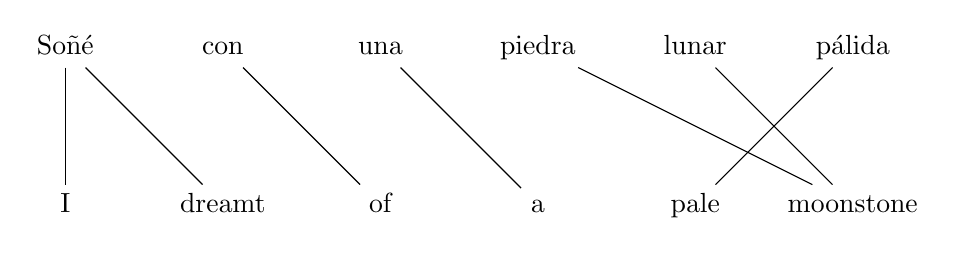
\begin{tikzpicture} [node distance = 2cm, text height=1.5ex, text depth=.25ex]
    % place nodes
    \node (Sone) {Soñé};
    \node [right of = Sone] (con) {con};
    \node [right of = con] (una) {una};
    \node [right of = una] (piedra) {piedra};
    \node [right of = piedra] (lunar) {lunar};
    \node [right of = lunar] (palida) {pálida};
    \node [below of = Sone] (I) {I};
    \node [right of = I] (dreamt) {dreamt};
    \node [right of = dreamt] (of) {of};
    \node [right of = of] (a) {a};
    \node [right of = a] (pale) {pale};
    \node [right of = pale] (moonstone) {moonstone};
    % draw edges
    \draw (Sone) -- (I);
    \draw (Sone) -- (dreamt);
    \draw (con) -- (of);
    \draw (una) -- (a);
    \draw (piedra) -- (moonstone);
    \draw (lunar) -- (moonstone);
    \draw (palida) -- (pale);
  \end{tikzpicture}
  \end{center}
  \caption{Example of word alignment $\bm{a}$ for a Spanish-English sentence pair.
    $\bm{f}$ is the Spanish sentence, $\bm{e}$ is the English sentence.
    The source (Spanish)
    length $J$ is 6 as well as the target (English) length $I$. This alignment
    exhibits many-to-one mappings (\emph{I} and \emph{dreamt} align
    to \emph{Soñé}), one-to-many mappings (\emph{moonstone} aligns
    to \emph{piedra} and \emph{lunar}), as well as crossing links
    (the link \emph{pale}---\emph{pálida} crosses the
    link \emph{moonstone}---\emph{lunar}).}
  \label{fig:examplealign}
\end{figure}
%

\citet{brown-dellapietra-dellapietra-mercer-1993} introduce the
alignment $\bm{a}$ as a latent variable in the translation model
$p(\bm{f} \mid \bm{e})$, as in \autoref{eq:introduceAlignment}:
\begin{equation}
  p(\bm{f} \mid \bm{e}) = \sum_{\bm{a}} p(\bm{f}, \bm{a} \mid \bm{e})
  \label{eq:introduceAlignment}
\end{equation}
%
We abuse notation by calling $\bm{a}$ both the latent variable
and the set of alignment links, which is an instance of the latent
variable.
For mathematical convenience and in order to allow simplifications,
given a sentence pair $(\bm{f}, \bm{e})$ with source length
$J$ and target length $I$,
$\bm{a}$ is restricted to be a function from source word positions
to target word positions, as in \autoref{eq:alignmentDefinition}:
%
\begin{equation}
\begin{split}
  \bm{a} : [1, J] &\longrightarrow [0, I] \\
                j &\longmapsto a_j
\end{split}
\label{eq:alignmentDefinition}
\end{equation}
%
The target position zero is included to
model source words not aligned to any target word; these unaligned source words
are virtually aligned to a so-called \emph{null word}. Note that this definition
is not symmetric: it only allows many-to-one mapping from source to target.
Various symmetrisation strategies, presented in \autoref{sec:symmetrisationHeuristics},
have been devised to address this limitation.
Also note that we did not
take into account the null word in our initial definition of alignments
in \autoref{eq:alignmentSetDefinition} because in general, alignments
are obtained from symmetrisation heuristics
(see \autoref{sec:symmetrisationHeuristics}) where the null word
is ignored.
We can use the latent variable
$\bm{a}$ to rewrite the translation model in
\autoref{eq:generalEquationIBMModels}, with $\bm{f} = f_1^J$, $\bm{e} = e_1^I$
and $\bm{a} = a_1^J$:
%
\begin{equation}
  \begin{split}
    p(f_1^J \mid e_1^I) &= \sum_{a_1^J} p(f_1^J, a_1^J \mid e_1^I) \\
                        &= \sum_{a_1^J} \prod_{j = 1}^J p(f_j, a_j \mid f_1^{j - 1}, a_1^{j - 1}, e_1^I) \\
                        &= \sum_{a_1^J} \prod_{j = 1}^J p(f_j \mid f_1^{j - 1}, a_1^j, e_1^I) \, p(a_j \mid f_1^{j - 1}, a_1^{j - 1}, e_1^I) \\
  \end{split}
  \label{eq:generalEquationIBMModels}
\end{equation}
%
\citet{brown-dellapietra-dellapietra-mercer-1993} present a series
of five translation models of increasing complexity that parameterise the terms
$p(f_j \mid f_1^{j - 1}, a_1^j, e_1^I)$ and
$p(a_j \mid f_1^{j-1}, a_1^{j-1}, e_1^I)$.
Parameter estimation is carried out with the
expectation-maximisation algorithm~\citep{dempster-laird-rubin:1977:JRSS}.
Also based on \autoref{eq:generalEquationIBMModels}, \citet{vogel-ney-tillmann}
introduce an HMM model for word alignment and \citet{deng-and-byrne:2008:ASLP}
extend the HMM model to a word-to-phrase HMM model. We describe these two models in the following
sections.
% TODO should I present all IBM models ???

% TODO think about where to put this
We have described word alignment models in the context of the source-channel
model. In that context, word alignment models can be used directly for word-based
decoding.\footnote{e.g. \url{http://www.isi.edu/licensed-sw/rewrite-decoder}} % TODO check whether MTTK and/or GIZA++ can also be used in decoding mode
However, nowadays, word alignment models are used as a preliminary
step in the machine translation training pipeline, namely
prior to rule extraction (see \autoref{sec:phrasextract} and
\autoref{sec:hierruleextract}). In that case,
the word alignment models are used to produce Viterbi alignments, defined
in \autoref{eq:viterbiAlignment}:
%
\begin{equation}
  %\begin{split}
    %\hat{a}_1^J &= \argmax_{a_1^J} p(a_1^J \mid f_1^J, e_1^I) \\
    \hat{a}_1^J = \argmax_{a_1^J} p(f_1^J, a_1^J \mid e_1^I)
  %\end{split}
  \label{eq:viterbiAlignment}
\end{equation}
%
One contribution of this
thesis is to use alignment posterior probabilities instead of
Viterbi alignments for rule
extraction (see \autoref{chap:extractionFromPosteriors}).

\subsection{HMM and Word-to-Phrase Alignment Models}
\label{sec:statisticalMachineTranslationHmmAlignmentModel}

% notes on Yonggang's 2008 journal paper
%in the paper notation, assuming translation is from foreign to English,
%source denotes English (target in thesis notation) and target denotes
%foreign (source in thesis notation)
%source sentence of I words s = s_1^I
%target sentence of J words t = t_1^J
%target sentence segmented into K target phrases
%target phrases: v_1^K
%each v_k generated by a single word in the source phrase
%correspondence source words target phrases: alignment a_1^K
%s_{a_k} -> v_k
%number of words in each target phrase: phi_k
%constraint: J = sum_{k=1}^K phi_k
%NULL source word
%alternative to NULL word: h_1^K hallucination sequence
%h_k = 0: NULL -> v_k; h_k = 1: s_{a_k} -> v_k
%a = (phi_1^K, a_1^K, h_1^K, K)
%p(t,a|s) = p(v_1^K, K, a_1^K, h_1^K, phi_1^K | s)


We review HMM and word-to-phrase HMM models as these models are used
in experiments throughout this thesis.
\citet{vogel-ney-tillmann} introduce an HMM alignment model
that treats target word positions as hidden states and source words as
observations. The model is written in \eqref{eq:HmmAlignmentDefinition}:
%
\begin{equation}
  p(f_1^J, a_1^J \mid e_1^I) = \prod_{j=1}^J p(a_j \mid a_{j-1},I) \, p(f_j \mid e_{a_j})
  \label{eq:HmmAlignmentDefinition}
\end{equation}
%
Word-to-phrase HMM models~\citep{deng-and-byrne:2008:ASLP} were designed to
capture interesting properties of IBM Model
4~\citep{brown-dellapietra-dellapietra-mercer-1993} in an HMM framework in order
to keep alignment and estimation procedures exact. We now present this model
in more detail, using our usual source/target convention, which is the reverse
than the one adopted in the original
publication\footnote{$\bm{s}$ in the publication corresponds to $\bm{e}$ in this thesis;
$\bm{t}$ corresponds to $\bm{f}$; $J$ corresponds to $J$; $I$ corresponds to $I$.}.
In the word-to-phrase HMM alignment model, the source sentence
$\bm{f}$ is segmented into source phrases $v_1^K$.
The alignment $\bm{a}$ is represented by a set of variables
$(\phi_1^K, a_1^K, h_1^K, K)$ where:
%
\begin{itemize}
  \item $K$ is the number of source phrases that form a segmentation of the source sentence $\bm{f}$.
  \item $a_1^K$ is the alignment from target words to source phrases.
  \item $\phi_1^K$ indicates the length of each source phrase.
  \item $h_1^K$ is a \emph{hallucination} sequence that indicates whether
    a source phrase was generated by the target null word
    or by a usual target word.
\end{itemize}
%
The general form of the model is presented in \autoref{eq:word2phraseHmmGeneral}:
%
\begin{equation}
  \begin{split}
  p(\bm{f}, \bm{a} \mid \bm{e}) = & \; p(v_1^K, K, a_1^K, h_1^K, \phi_1^K \mid \bm{e}) \\
                                = & \; p(K \mid J, \bm{e}) \times \\
                                & \; p(a_1^K, \phi_1^K, h_1^K \mid K, J, \bm{e}) \times \\
                                & \; p(v_1^K \mid a_1^K, h_1^K, \phi_1^K, K, J, \bm{e})
  \end{split}
  \label{eq:word2phraseHmmGeneral}
\end{equation}
%
We now review the modelling decisions taken for each
of the components from \autoref{eq:word2phraseHmmGeneral}.
The first component is simply modelled by:
%
\begin{equation}
  p(K \mid J, \bm{e}) = \eta^K
\end{equation}
%
where $\eta$ is a threshold that controls the number of segments in the source.
The second component is modelled using the Markov assumption:
%
\begin{align}
  p(a_1^K, \phi_1^K, h_1^K \mid K, J, \bm{e})
    &= \prod_{k = 1}^K p(a_k, h_k, \phi_k \mid a_{k - 1}, \phi_{k - 1}, h_{k - 1}, K, J, \bm{e}) \nonumber \\
    &= \prod_{k = 1}^K p(a_k \mid a_{k - 1}, h_k, I) \, d(h_k) \, n(\phi_k \mid e_{a_k})
\end{align}
%
As in the HMM word alignment model $a_k$ depends only on $a_{k - 1}$, the target
length $I$ and the binary value $h_k$. $d(h_k)$ is simply controlled by the
parameter $p_0$ by $d(0) = p_0$. $n(\phi_k \mid e_{a_k})$ is a finite distribution
on source phrase length that depends on each target word and which plays the role
of a fertility parameter.

The third component from \autoref{eq:word2phraseHmmGeneral} is defined in
\autoref{eq:word2phraseTranslation} and represents the word-to-phrase translation parameter:
%
\begin{equation}
  p(v_1^K | a_1^K, h_1^K, \phi_1^K, K, J, \bm{e}) = \prod_{k = 1}^K p(v_k \mid e_{a_k}, h_k, \phi_k)
  \label{eq:word2phraseTranslation}
\end{equation}
%
One key contribution from the word-to-phrase HMM model is to use bigram translation
probabilities to model one single phrase translation, as shown
in \autoref{eq:bigramTranslation}:
%
\begin{equation}
  p(v_k \mid e_{a_k}, h_k, \phi_k) = t_1(v_k[1] \mid h_k \cdot e_{a_k}) \prod_{j = 2}^{\phi_k} t_2(v_k[j] \mid v_k[j - 1], h_k \cdot e_{a_k})
  \label{eq:bigramTranslation}
\end{equation}
%
where $h_k \cdot e_{a_k}$ is $e_{a_k}$ if $h_k = 1$ and the null word otherwise, $t_1$ is
a word-to-word translation probability and $t_2$ is a bigram translation probability.

\autoref{fig:wordtophrase}
shows a simplified version of the generative story for an HMM word-to-phrase
alignment model: first, pick the number of source phrases $K$ according to
$P(K \mid J,I)$; then
pick a target word given the previously chosen one; finally generate the target
phrase from the source word using fertility and bigram translation probabilities.
For example, we generate the source phrase \emph{les vaches} from
the target word \emph{cows}
according to \autoref{eq:exampleBigramTranslation}:
%
\begin{equation}
  p(\text{\emph{les vaches}} \mid \text{\emph{cows}}) = p(\text{\emph{les}} \mid \text{\emph{cows}}) \, p(\text{\emph{vaches}} \mid \text{\emph{cows}}, \text{\emph{les}})
  \label{eq:exampleBigramTranslation}
\end{equation}
%
Thus bigram probabilities take into account the context of the target word to
some extent.
%
%\begin{figure}
%  \begin{center}
%    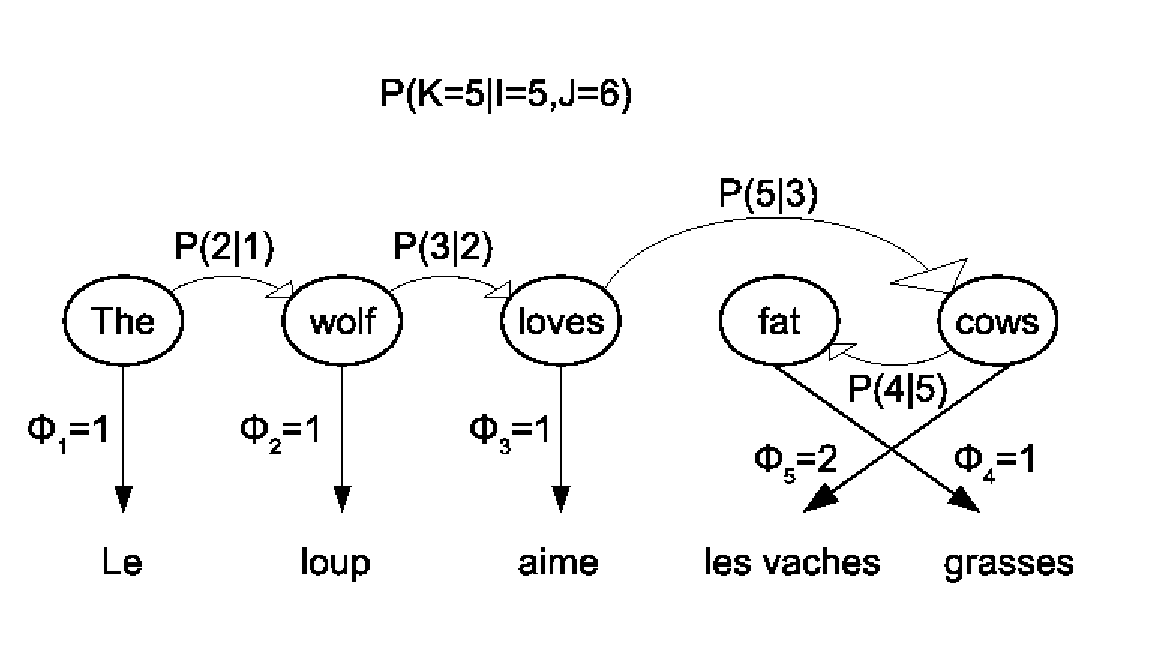
\includegraphics[scale=0.5]{figures/wordtophrase2.eps}
%  \end{center}
%  \caption{Illustrative example of an HMM word-to-phrase alignment model. The adjective noun sequence ``fat cows'' is
%    reordered into the noun adjective sequence ``vaches grasses''. The word ``cows'' has fertility 2 as it is translated
%    into the target phrase ``les vaches''.}
%  \label{fig:wordtophrase}
%\end{figure}
\begin{figure}
  \begin{center}
  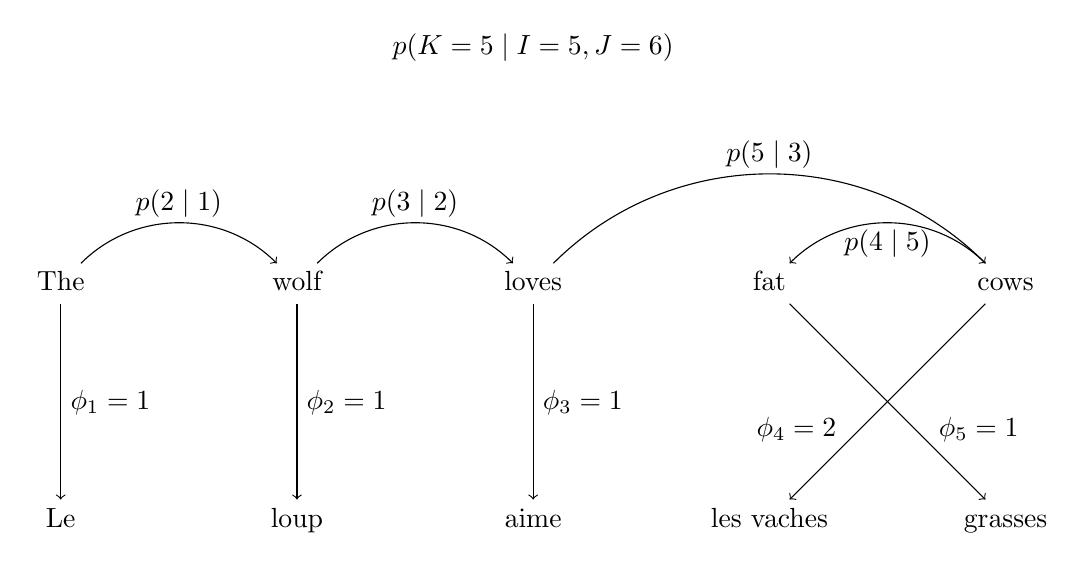
\begin{tikzpicture} [node distance = 3cm, text height=1.5ex, text depth = .25ex, auto]
    % place nodes
    \node (the) {The};
    \node [right of = the] (wolf) {wolf};
    \node [right of = wolf] (loves) {loves};
    \node [right of = loves] (fat) {fat};
    \node [right of = fat] (cows) {cows};
    \node [above of = loves] (chooseSeg) {$p(K = 5 \mid I = 5, J = 6)$};
    
    \node [below of = the] (le) {Le};
    \node [below of = wolf] (loup) {loup};
    \node [below of = loves] (aime) {aime};
    \node [below of = fat] (lesVaches) {les vaches};
    \node [below of = cows] (grasses) {grasses};

    % draw edges
    \draw [->] (the) to node {$\phi_1 = 1$} (le);
    \draw [->] (wolf) to node {$\phi_2 = 1$} (loup);
    \draw [->] (loves) to node {$\phi_3 = 1$} (aime);
    \draw [->] (fat) to node [right, xshift = 1.5em, yshift = -1em] {$\phi_5 = 1$} (grasses);
    \draw [->] (cows) to node [left, xshift = -1.5em, yshift = -1em] {$\phi_4 = 2$} (lesVaches);

    \draw [->] (the) to [bend left = 45] node {$p(2 \mid 1)$} (wolf);
    \draw [->] (wolf) to [bend left = 45] node {$p(3 \mid 2)$} (loves);
    \draw [->] (loves) to [bend left = 45] node {$p(5 \mid 3)$} (cows);
    \draw [->] (cows) to [bend right = 45] node {$p(4 \mid 5)$} (fat);
  \end{tikzpicture}
  \end{center}
  \caption{Simplified generative story for an HMM word-to-phrase alignment model.
    Adapted from~\citep{deng-and-byrne:2008:ASLP}.
    The adjective noun sequence \emph{fat cows} is
    reordered into the noun adjective sequence \emph{vaches grasses}.
    The word \emph{cows} has fertility 2 as it is translated
    into the target phrase \emph{les vaches}.}
  \label{fig:wordtophrase}
\end{figure}

\subsection{Symmetrisation Heuristics}
\label{sec:symmetrisationHeuristics}

We have mentioned that the IBM and HMM alignment models
are not symmetric: they only allow a many-to-one mapping from
source words to target words.
In order to address this issue, one can train
alignment models in both source-to-target and target-to-source
directions, obtain Viterbi alignments from
both models and apply symmetrisation
strategies~\citep{och-tillmann-ney:1999:EMNLP,och-ney:2003:CL,koehn-och-marcu:2003:NAACL}.
\citet{och-tillmann-ney:1999:EMNLP} designed
a first symmetrisation heuristic that was later on dubbed
as the \emph{grow} heuristic. \citet{koehn-och-marcu:2003:NAACL}
later extend the \emph{grow} heuristic into
the \emph{grow-diag} and \emph{grow-diag-final} heuristics
and examine the impact on translation
performance for each heuristic.

Alignments from source to target (i.e. the alignment is
a function from source positions to target positions)
and target to source are denoted
$\bm{a}_{f2e}$ and $\bm{a}_{e2f}$ respectively.
Let us consider a sentence pair $(\bm{f}, \bm{e})$, and
source-to-target and target-to-source Viterbi alignments
$\bm{a}_{f2e}$ and $\bm{a}_{e2f}$.
The \emph{intersection} and \emph{union} heuristics
are defined as follows:
%
\begin{itemize}
  \item \emph{intersection}: $\bm{a} = \bm{a}_{e2f} \cap \bm{a}_{f2e}$
  \item \emph{union}: $\bm{a} = \bm{a}_{e2f} \cup \bm{a}_{f2e}$
\end{itemize}
%
The \emph{intersection} heuristics typically produces high precision alignments
while the \emph{union} heuristics typically produces high recall alignments.
We now present the \emph{grow} heuristic and its variants, which are based
on the initial \emph{intersection} and \emph{union} heuristics.
The \emph{grow} heuristic algorithm is presented in
\autoref{alg:growHeuristic}. The input is a sentence
pair $(f_1^J, e_1^I)$, a source-to-target
alignment $\bm{a}_{f2e}$ and a target-to-source alignment
$\bm{a}_{e2f}$. The resulting alignment $\bm{a}$ is initialized
with the
intersection (\hyperlink{alg:line:initGrow}{line \ref{alg:line:initGrow}}).
Then alignment links that are in the union and that are neighbours of already existing
alignment links (\hyperlink{alg:line:neighbours}{line \ref{alg:line:neighbours}})
are considered. If the source or the target word is not already
aligned (\hyperlink{alg:line:notAlreadyAligned}{line \ref{alg:line:notAlreadyAligned}}),
then the link is added to the resulting
alignment (\hyperlink{alg:line:addLink}{line \ref{alg:line:addLink}}).
This is repeated until no more links are added.
%
\begin{figure}
  %\begin{footnotesize}
  \begin{algorithmic}[1]
    \Function{Grow}{$f_1^J, e_1^J, \bm{a}_{f2e}, \bm{a}_{e2f}$}
      \State{$\bm{a} \gets \bm{a}_{f2e} \cap \bm{a}_{e2f}$} \hypertarget{alg:line:initGrow}{} \label{alg:line:initGrow}
      \While{\textbf{true}}
        \State{added $\gets$ \textbf{false}}
        \For{$i \in [1, I]$}
          \For{$j \in [1, J]$}
            \If{$(j, i) \in \bm{a}$}
            \For{$(k, l) \in $ \Call{Neighbours}{$(j,i)$} $\cap (\bm{a}_{f2e} \cup \bm{a}_{e2f})$} \hypertarget{alg:line:neighbours}{} \label{alg:line:neighbours}
              \If{$k$ not aligned in $\bm{a}$ \textbf{or} $l$ not aligned in $\bm{a}$} \hypertarget{alg:line:notAlreadyAligned}{} \label{alg:line:notAlreadyAligned}
                \State{$\bm{a} \gets \bm{a} \cup (k, l)$} \hypertarget{alg:line:addLink}{} \label{alg:line:addLink}
                \State{added $\gets$ \textbf{true}}
              \EndIf
            \EndFor
            \EndIf
          \EndFor
        \EndFor
        \If{not added} 
          \State{\textbf{break}}
        \EndIf
      \EndWhile
      \State{\Return $\bm{a}$}
    \EndFunction
  \end{algorithmic}
  %\end{footnotesize}
  \caption{Algorithm for the \emph{grow} symmetrisation heuristic.
    The alignment is initialized from the intersection and alignment links
    that are neighbours to existing alignment links are iteratively added if the source
    or the target is not already aligned.}
  \label{alg:growHeuristic}
\end{figure}

In the \emph{grow} heuristic, neighbours are defined as horizontal or
vertical neighbours. If diagonal neighbours are also considered, then
the heuristic becomes \emph{grow-diag}. The \emph{grow} heuristic
also has an optional step called \emph{final}. Alignment
links in the union where the source or the target is not already
aligned can also be added to the resulting alignment. If only links
in the union where the source \emph{and} the target are not already
aligned are considered for the \emph{final} procedure, then
the optional step is called \emph{final-and}.

Symmetrisation heuristics have been shown to be beneficial for
alignments both in terms of alignment quality as measured
by comparing automatic alignments to human alignments and
in translation quality when alignments are used as an
intermediate step in the translation pipeline.

%
%Symmetrised alignments have be shown to produce better translation results than
%unidirectional alignments. However, we find in one of our experiments that this
%is not always the case (see \autoref{sec:extractionFromPosteriorsSymmetrising}).

% This should review phrase based SMT.
% Why: the gyro decoder is like a phrase based SMT decoder.

% phrase based extraction + stack base decoding

\section{Log-Linear Model of Machine Translation}
\label{sec:loglinearModel}

%notes on adam berger paper
%model conditional prob
%p(y | x): x is phrase containing word "in", y is translation of "in"
%collect stats ptilda(x, y)
%binary feature: f(x, y) = 1 if y = en and April follows in
%expected value of f: ptilda(f) = sum_x,y ptilda(x,y) f(x,y)
%p(f) = sum_x,y ptilda(x) p(y | x) f(x,y)
%constraint: p(f) = ptilda(f)
%max entropy principle: choose p that satisfies the constraints
%and that maximizes entropy
%H(p) = -sum_x,y ptilda(x) p(y|x) log p(y|x)
%use Lagrange multiplier and Kuhn Tucker theorem to find that the solution
%is p(y|x) propto exp(\sum lambda_i f_i(x,y)). find lambda by max dual problem.
%also: p that satisfies constr and max entropy is also the
%p in the parametric family ... that maximizes likelihood of training sample.
%application to Candide.
%use max entropy modelling to predict translation of word in context.
%use max entropy modelling to predict word order.
%use max entropy modelling to segment.
%context dependent translation:
%first viterbi align training. then create events (x,y) (6 words
%surrounding in)
%incorporate this context dep translation into general translation model.

As we have seen in \autoref{sec:sourceChannelModel}, SMT was historically
framed as a source-channel model. As an alternative,
\citet{berger-dellapietra-dellapietra:1996:CL} introduce maximum entropy
models for natural language processing. In maximum entropy modelling, we
wish to estimate a conditional probability $p(\bm{y} \mid \bm{x})$.
Given a training sample, various feature functions deemed to be relevant
are picked. We then constrain $p$ such that the expected value of each
feature function $f$ with respect to the empirical distribution is equal
to the expected value of $f$ with respect to the model $p$. Finally, $p$
is chosen among all models that satisfy the constraints defined by the
features and such that its entropy is maximum.
\citet{berger-dellapietra-dellapietra:1996:CL} show how a maximum entropy
model can be parameterized as an exponential, or log-linear model. They
apply this model to three machine translation related tasks. First, they
use a maximum entropy model to predict the translation of a word using
the context for that word. Then, they use a maximum entropy model to
predict the target language word order. Finally, they apply maximum
entropy modelling in order to predict the source sentence segmentation.

%notes och and ney 2002
%search done by the maximum approximation
%first present log linear model
%log linear model generalization of source channel model
%log linear model presented with additional alignment variable
%p(e_1^I, a_1^J | f_1^J) propto exp(sum_1^M lambda_m h_m(e_1^I, f_1^J, a_1^J))
%alignment template model
%p(f_1^J | e_1^I) = sum_{z_1^K, a_1^K} p(a_1^K | e_1^I) . p(z_1^K | a_1^K, e_1^I) . p(f_1^J | z_1^K, a_1^K, e_1^I)
%each component modeled with max entropy model

\citet{och-tillmann-ney:1999:EMNLP} notice that using an erroneous
version of the source-channel model, that is using the following equation:
%
\begin{equation}
  \bm{\hat{e}} = \argmax_{\bm{e}} p(\bm{e} \mid \bm{f}) \, p(\bm{e})
\end{equation}
%
give comparable performance with respect to using the correct
formulation of the source-channel model given in \autoref{eq:noisy}.
Then \citet{och-ney:2002:ACL} propose the following log-linear model extension:
%
\begin{align}
  \bm{\hat{e}} &= \argmax_{\bm{e}} p(\bm{e} \mid \bm{f}) \nonumber \\
               &= \argmax_{\bm{e}} \frac{\exp(\sum_{m=1}^M \lambda_m h_m(\bm{e}, \bm{f}))}{\sum_{\bm{e'}}\exp(\sum_{m=1}^M \lambda_m h_m(\bm{e'}, \bm{f}))} \nonumber \\
               &= \argmax_{\bm{e}} \exp(\sum_{m=1}^M \lambda_m h_m(\bm{e}, \bm{f})) \label{eq:loglinearModel}
\end{align}
%
where $h_m$ are called \emph{feature functions} and $\lambda_m$
are called \emph{feature weights}. The log-linear model is an extension
to the noisy channel model because it can be reduced to the original
noisy channel model with the following settings:
%
    \begin{itemize}
      \item $M = 2$
      \item $h_1(\bm{e}, \bm{f}) = \log (p(\bm{f}|\bm{e}))$
      \item $h_2(\bm{e}, \bm{f}) = \log (p(\bm{e}))$
      \item $\lambda_1 = \lambda_2 = 1$
    \end{itemize}
%
Log-linear models were originally trained with the maximum likelihood
criterion, which precisely makes them equivalent to maximum entropy
models~\citep{berger-dellapietra-dellapietra:1996:CL}. However,
more effective training techniques such as minimum error rate
training~\citep{och:2003:ACL} were introduced later on, that do
not require the computation of the normalization constant
(see \autoref{sec:mert}).
Thus, in practice, SMT models are effectively simply linear models, with the objective
function presented in \autoref{eq:linearModel}:
%
\begin{equation}
  \bm{\hat{e}} = \argmax_{\bm{e}} \sum_{m=1}^M \lambda_m h_m(\bm{e}, \bm{f})
  \label{eq:linearModel}
\end{equation}

%In practice, \citet{och-ney:2002:ACL} do not use \autoref{eq:loglinearModel}.
%They introduce several latent variables in a so called \emph{alignment template}
%approach. The translation model is defined in \autoref{eq:alignmentTemplate}:
%
%\begin{equation}
%  p(e_1^I \mid f_1^J) = \sum_{z_1^K, a_1^K} p(a_1^K \mid e_1^I) p(z_1^K \mid a_1^K, e_1^I) p(f_1^J \mid z_1^K, a_1^K, e_1^I)
%  \label{eq:alignmentTemplate}
%\end{equation}
%
% TODO check if it is "correct" to invert the notation in above equation wrt to original publication
%where the variables $z_1^K$ and $a_1^K$ are alignment templates and the alignment of alignment templates.
%Each term in \autoref{eq:alignmentTemplate} is modelled as a maximum entropy model and search
%is carried out using the maximum approximation defined in \autoref{eq:maxApproximation}:
%
% TODO finish this
%\begin{align}
%  \hat{e_1^I} &= \argmax_{z_1}
%  \label{eq:maxApproximation}
%\end{align}

% TODO talk about training methods: GIS vs MERT

\section{Phrase-Based Translation}
\label{sec:phraseBasedTranslation}

%notes on och et al 1999
%compare word based and phrase based
%e = argmax p(e) p(f|e)
%word based model: each source word (french) assigned exactly one target word (english)
%difficult to model context and also to translate compound words
%model two alignment levels: phrase level alignment between phrases and word level alignment between words within phrases
%word based approach: use an HMM
%p(f_1^J | e_1^I) = sum_{a_1^J} prod_j p(a_j | a_{j - 1}) p(f_j | e_{a_j})
%some restrictions are used (so called monotonicity): alignment jump between a_{j - 1} and a_j can only be 0, 1, 2.
%Q_{e'}(j, e): probability of best partial hypothesis (e_1^i, a_1^j) with e_i = e, e_{i - 1} = e' and a_j = i
%search: mapping j -> (a_j, e_{a_j})
%DP recursion:
%Q_e'(j, e) = p(f_j | e) . max {
%  p(0) . Q_e'(j - 1, e),
%  p(1) . max_e'' {p(e | e', e'') Q_e''(j - 1, e')},
%  p(2) . max_{e'', e'''} {p(e | e', e'') . p(e' | e'', e''') . Q_e'''(j - 1, e'')}
%  }
%optimal translation: max_e',e Q_e'(J, e) . p(\$ | e, e')
%extension to one-to-many alignment model.
%solution: reverse translation direction, then extend English vocab with multiple words, then redo standard training for original translation direction.
%alignment template approach
%problem with word based models: only allow one to many or many to one, or many to many but hacky solution
%model phrase to phrase is a way to model context.
%alignment template z: triple (Ftilda, Etilda, Atilda) alignment Atilda between source class sequence Ftilda and
%target class sequence Etilda.
%Atilda: matrix with binary values
%Atilda allows for many to many
%Ftilda and Etilda automatically trained bilingual classes
%use classes for better generalization
%alignment template applicable to sequence source words ftilda if
%alignment template classes and classes of source words are equal
%application of alignment template contraints the target words to have the right classes
%selection target words: p(etilda | z, ftilda)
%p(ftilda | (Ftilda, Etilda, Atilda), etilda) = delta(classes(etilda), Etilda) delta(classes(ftilda), Ftilda) prod_{j=1}^J (I???) p(f_j | Atilda, etilda)
%p(f_j | Atilda, etilda) = sum_{i = 0}^I p(i | j; Atilda) p(f_j | e_i)
%p(i | j, Atilda) = Atilda(i, j) / (sum_i Atilda(i, j))
%rien compris
%phrase level alignment
%decompose f_1^J and e_1^I into sequence of phrases
%f_1^J = ftilda_1^K
%assume that there is only one possible segmentation (possibly one of the differences between Och and Koehn)
%p(f_1^J | e_1^I) = p(ftilda_1^K | etilda_1^K)
%                 = sum_{atilda_1^K} p(atilda_1^K, ftilda_1^K | etilda_1^K)
%                 = sum_{atilda_1^K} p(atilda_1^K | etilda_1^K) p(ftilda_1^K | atilda_1^K, etilda_1^K)
%                 = sum_{atilda_1^K} prod_{k = 1}^K p(atilda_k | atilda_1^{k-1}, K) p(ftilda_k | etilda_{atilda_k})
%p(ftilda | etilda) = sum_z p(z| etilda) p(ftilda | z, etilda)
%training: s2t and t2s hmm without the max approximation
%get the viterbi alignments a_1^J and b_1^I
%use the grow diag symmetrisation heuristic.
%estimate bilingual word lexicon p(f|e): n_A(f, e) | n(e)
%train world classes
%extract consistent phrase pairs from alignment
%obtain n(z) of how often alignment template occurs in aligned corpus.
%relative freq estimate: p(z = (Ftilda, Etilda, Atilda) | etilda) = n(z) . delta(classes(etilda), Etilda) / n(classes(etilda))
%decoding search
%objective: argmax_{e_1^I} p(e_1^I p(e_1^I | f_1^J)) (wrong version of source channel model)
%use class-based 5g lm
%preprocessing before translation: filter alignment templates per source sentence, segment source sentence
%segmentation objective: argmax_{ftilda_1...ftilda_k = f_1^J} prod_{k=1}^K max_z p(z | ftilda_k)
%search: produce partial hypotheses with info: last target word, language model state,
%source coverage, last alignment template, position of last target word in alignment template
%instantiation (???), cost so far, backpointer
%integrate future cost because compare hypotheses that cover different parts of the input

%notes on och-ney 2004 (journal paper version of och et al. 1999)
%overview: align, extract, extracted phrases with alignment and word classes are
%called alignment templates
%log-linear model: hat{e_1^I} = argmax_{e_1^I} p(e_1^I | f_1^J)
%                             = argmax exp(sum_m=1^M lambda_m h_m(e_1^I, f_1^J))/Z
%parameters lambda trained with MLE (same as maximum entropy)
%or trained with MERT
%use latent variable
%p(e_1^I, a_1^J | f_1^J) = (1/Z) . exp(sum_1^M lambda_m h_m(e_1^I, f_1^J, a_1^J))
%description of word alignments etc.
%description of symmetrisation heuristics etc.
%symmetrized Viterbi alignments used to compute translation lexicon
%description of phrase-extract
%alignment templates: replace words with word classes and store
%alignment info for each phrase pair
%alignment template z = (F_1^J', E_1^I', Atilda)
%F_1^J' source class sequence
%E_1^I' target class sequence
%Atilda: alignment between source class seq and target class seq
%automatically train bilingual classes
%notation: etilda, ftilda target and source phrases
%p(z = (F_1^J', E_1^I', Atilda) | ftilda) = N(z) . delta(F_1^J', C(ftilda)) / N(C(ftilda%))
%remove alignment templates with prob less than 0.01
%limit on source phrase: between 4 and 7
%translation model
%f_1^J = ftilda_1^K
%e_1^I = etilda_1^K
%model described for a specific segmentation but in search
%optimal segmentation also searched for
%pi_1^K: permutation of the phrases, models phrase reordering
%etilda_k is translation of ftilda_{pi_k}
%alignment template between f_{pi_k} and e_k: z_k
%hidden variables in the model: pi_1^K, z_1^K
%use log-linear model, feature functions depend on source, target and hidden variables
%features
%alignment template selection
%h_AT(e_1^I, f_1^J, pi_1^K, z_1^K) = log prod_1^K p(z_k | f_{j_{pi_k - 1} + 1}^{j_{pi_k}%})
%h_WRD(e_1^I, f_1^J, pi_1^K, z_1^K) = log prod_1^I p(e_i | {f_j, (i,j) in A}, E_i)
%p(e_i | {f_j, (i,j) in A}, E_i)
%etc etc. hyper complique
%h_AL phrase alignment (reordering model)
%h_AL(e_1^I, f_1^J, pi_1^K, z_1^K) = sum_{k=1}^{K+1} |j_{pi_k - 1} - j_{pi_{k - 1}}
%3gram lm + 5g class based lm
%training: blabla
%search
%breadth-first search with pruning: beam search
%search objective:
%hat{e_1^I} = argmax_{e_1^I} sum_{pi_1^K, z_1^K} p(e_1^I, z_1^K, pi_1^K | f_1^J)
%           ~~ argmax_{e_1^I, pi_1^K, z_1^K} p(e_1^I, z_1^K, pi_1^K | f_1^J)
%           = argmax_{e_1^I, pi_1^K, z_1^K} sum_{m = 1}^M lambda_m h_m(e_1^I, f_1^J, pi_%1^K, z_1^K)
%use the max approximation
%structure of search space
%generate hypothesis left to right on the target
%preprocessing step: first determine all source phrases that match an alignment template
%unknown words carried over
%use 5-best target words for each target class according to some criterion
%use hypothesis recombination
%pruning done for hypotheses that cover the same number of source words
%future cost estimation
%rien compris
%exps etc. etc.

%notes on phrase-based mt by koehn's book
%EM training of phrase-based models: NO
%Extensions to the Reordering Model
%zh-en, ar-en, fr-en in contrast to de-en or jp-en
%lexicalized reordering
%reordering model p_o predicts orientation m,s,d given phrase pair f,e:
%p_o(orientation | f, e)
%extract each phrase pair with orientation type p_o(orientation | f, e) = count(orientation, e, f) / sum_o count(o, e, f)
%to be smoothed with prior p_o(orientation)
%phrase translation as classification: use max ent model to model context
%use phrase penalty to model source segmentation
%use word penalty to model length
%lexical weighting a la koehn
%used as smoothing for translation model
%lex(e|f, a) = prod_{i = 1}^length(e) (1/|{j | (i,j) in a}|) sum_{j | (i,j) in a} w(e_i | f_j)
%if english word unaligned, use the NULL word on the f side
%w estimated with rel freq from aligned corpus.
%use both lex(e|f,a) and lex(f|e,a)
%log linear model: TODO find out what's the objective in moses/koehn2003
%phrase-extract etc. etc.
%source channel phrase-based model:
%e = argmax p(f|e) p(e)
%  = argmax prod_i p(f_i | e_i) d(start_i - end_{i - 1} -1)
%justification: segmentations are equally likely, max approximation ??
%d(x) propto alpha^|x|

%notes on phrase-based mt decoding by koehn's book
%description of hypothesis expansion
%computational complexity: NP complete/hard
%hypothesis recombination
%simple example: [it] [is] vs. [it is]
%more complicated example: [he] [does not] vs. [it] [does not]
%note: instead of deleting the hyp, we still keep pointer
%so that we can output n-best
%stack decoding
%stack <-> number of foreign words translated
%problem: some hyps in a stack cover different regions of the input
%histogram pruning and threshold pruning
%reordering limit in search
%future cost or outside cost or rest cost
%cost of translation option: translation cost easy,
%language model cost approximated by lm without context,
%reordering model ignored
%for each translation option, compute the ``cost without context''
%then estimate the cheapest cost for translating any span in the
%input using DP
%use future cost in search: add the cost of the remaining (gappy) span
%to the partial cost

%notes on koehn et al 2003
%"Note that phrase translation with a lexical weight is a
%special case of the alignment template model [Och et al.,
%1999] with one word class for each word."

So far, we have presented two modelling approaches to machine translation:
the original source-channel model and the current log-linear model. We also
have presented word alignment models, which were introduced within the source-channel
model framework and which are instances of word-based models.

% TODO motivation for phrase based: word based a:[1,J]->[1,I] so many to one mapping only
In the phrase-based translation paradigm, the minimal unit of translation consists
of phrases. Phrases are sequences of consecutive words, that need not be syntactically
or semantically motivated.
Benefits of phrase-based models include:
%
\begin{itemize}
  \item effectively disambiguating the translation of a word in a certain local context;
  \item effective local reordering such as the adjective-noun inversion from French to English;
  \item effective translation of multi-word expressions.
\end{itemize}
%
Phrase-based models
currently achieve state-of-the-art performance for
certain language pairs that do not involve much reordering
such as French-English. They can be defined
in the source-channel model framework (see \autoref{sec:sourceChannelModel}) or
the log-linear model framework (see \autoref{sec:loglinearModel}).
Because the source-channel model is rarely used anymore and because it is
a special case of a log-linear model, we will focus our presentation
on the log-linear model.

There are different variations on the phrase-based translation paradigm.
We will focus on two popular approaches, namely the alignment template
model~\citep{och-tillmann-ney:1999:EMNLP,och-ney:2004:CL} and the phrase-based
model~\citep{koehn-och-marcu:2003:NAACL,koehn:2010:book}.

\subsection{Alignment Template Model}

The alignment template model uses the log-linear model presented
in \autoref{eq:loglinearModel} as a starting point and repeated in
\autoref{eq:loglinearModelRepeated}:
%
\begin{equation}
  \bm{\hat{e}} = \argmax_{e_1^J} \exp(\sum_{m = 1}^M \lambda_m h_m(f_1^J, e_1^I))
  \label{eq:loglinearModelRepeated}
\end{equation}
%
In order to reduce the number of parameters, the two latent variables $\pi_1^K$
and $z_1^K$ are introduced. $z_1^K$ is a sequence of \emph{alignment templates}
while $\pi_1^K$ is a permutation of size $K$. An alignment template
is a triple $(\tilde{F}, \tilde{E}, \tilde{A})$ where $\tilde{F}$ is a
sequence of source word classes, $\tilde{E}$ is a sequence of target
word classes and $\tilde{A}$ is an alignment between $\tilde{F}$
and $\tilde{E}$. $\pi_1^K$ together with $z_1^K$ define
a source segmentation of $f_1^J$ into source phrases $\tilde{f}_1^K$,
a target segmentation of $e_1^I$ into target phrases $\tilde{e}_1^K$ and
a bijective mapping between source phrases and target phrases where
$\tilde{f}_{\pi_k}$ is mapped to $\tilde{e}_{k}$ for $k \in [1,K]$.
The alignment templates $z_1^K$ are constrained in such a way that
the alignment template classes match the word classes.
The alignment template translation model is summarized
in \autoref{fig:alignmentTemplateTranslationModel}.
%
\begin{figure}
  \begin{center}
    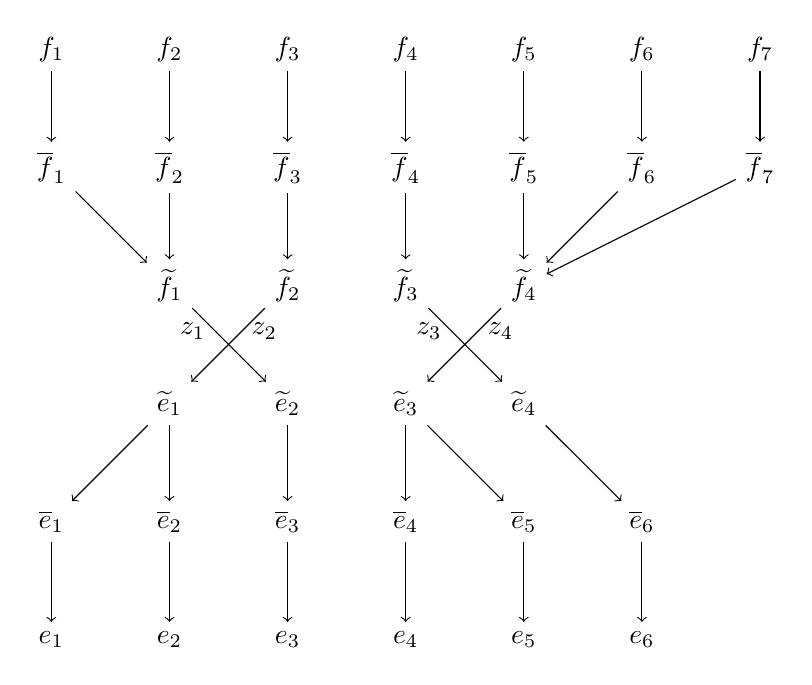
\begin{tikzpicture}[node distance = 1.5cm]
      % place nodes
      \node (f1) {$f_1$};
      \node (f2) [right of = f1] {$f_2$};
      \node (f3) [right of = f2] {$f_3$};
      \node (f4) [right of = f3] {$f_4$};
      \node (f5) [right of = f4] {$f_5$};
      \node (f6) [right of = f5] {$f_6$};
      \node (f7) [right of = f6] {$f_7$};

      \node (cf1) [below of = f1] {$\overline{f}_1$};
      \node (cf2) [below of = f2] {$\overline{f}_2$};
      \node (cf3) [below of = f3] {$\overline{f}_3$};
      \node (cf4) [below of = f4] {$\overline{f}_4$};
      \node (cf5) [below of = f5] {$\overline{f}_5$};
      \node (cf6) [below of = f6] {$\overline{f}_6$};
      \node (cf7) [below of = f7] {$\overline{f}_7$};

      \node (pf1) [below of = cf2] {$\widetilde{f}_1$};
      \node (pf2) [below of = cf3] {$\widetilde{f}_2$};
      \node (pf3) [below of = cf4] {$\widetilde{f}_3$};
      \node (pf4) [below of = cf5] {$\widetilde{f}_4$};

      \node (pe1) [below of = pf1] {$\widetilde{e}_1$};
      \node (pe2) [below of = pf2] {$\widetilde{e}_2$};
      \node (pe3) [below of = pf3] {$\widetilde{e}_3$};
      \node (pe4) [below of = pf4] {$\widetilde{e}_4$};

      \node (ce2) [below of = pe1] {$\overline{e}_2$};
      \node (ce1) [left of = ce2] {$\overline{e}_1$};
      \node (ce3) [below of = pe2] {$\overline{e}_3$};
      \node (ce4) [below of = pe3] {$\overline{e}_4$};
      \node (ce5) [below of = pe4] {$\overline{e}_5$};
      \node (ce6) [right of = ce5] {$\overline{e}_6$};

      \node (e1) [below of = ce1] {$e_1$};
      \node (e2) [below of = ce2] {$e_2$};
      \node (e3) [below of = ce3] {$e_3$};
      \node (e4) [below of = ce4] {$e_4$};
      \node (e5) [below of = ce5] {$e_5$};
      \node (e6) [below of = ce6] {$e_6$};
      % draw edges
      \draw [->] (f1) -- (cf1);
      \draw [->] (f2) -- (cf2);
      \draw [->] (f3) -- (cf3);
      \draw [->] (f4) -- (cf4);
      \draw [->] (f5) -- (cf5);
      \draw [->] (f6) -- (cf6);
      \draw [->] (f7) -- (cf7);

      \draw [->] (cf1) -- (pf1);
      \draw [->] (cf2) -- (pf1);
      \draw [->] (cf3) -- (pf2);
      \draw [->] (cf4) -- (pf3);
      \draw [->] (cf5) -- (pf4);
      \draw [->] (cf6) -- (pf4);
      \draw [->] (cf7) -- (pf4);

%      \draw[->] (P) to node {$\pi_{j}$} (B);

      \draw [->] (pf1) to node[left, xshift = -0.5em, yshift = 0.5em]{$z_1$} (pe2);
      \draw [->] (pf2) to node[right, xshift = 0.5em, yshift = 0.5em]{$z_2$} (pe1);
      \draw [->] (pf3) to node[left, xshift = -0.5em, yshift = 0.5em]{$z_3$} (pe4);
      \draw [->] (pf4) to node[right, xshift = 0.5em, yshift = 0.5em]{$z_4$} (pe3);

      \draw [->] (pe1) -- (ce1);
      \draw [->] (pe1) -- (ce2);
      \draw [->] (pe2) -- (ce3);
      \draw [->] (pe3) -- (ce4);
      \draw [->] (pe3) -- (ce5);
      \draw [->] (pe4) -- (ce6);

      \draw [->] (ce1) -- (e1);
      \draw [->] (ce2) -- (e2);
      \draw [->] (ce3) -- (e3);
      \draw [->] (ce4) -- (e4);
      \draw [->] (ce5) -- (e5);
      \draw [->] (ce6) -- (e6);
    \end{tikzpicture}
  \end{center}
  \caption{Alignment template translation process.
    Adapted from~\citep{och-ney:2004:CL}. The source word
  sequence $f_1^7$ is first transformed into a source class
  sequence $\overline{f}_1^7$. The source classes are then segmented
  into source phrases $\widetilde{f}_1^4$. The source phrases are then
  reordered and aligned to target phrases $\widetilde{e}_1^4$.
  For example, the source phrase $\widetilde{f}_1$ is aligned to
  the target phrase $\widetilde{e}_2$ through $z_1$.
  This means that the permutation $\pi_1^4$
  has value $\pi_2 = 1$. This also means that $z_1$
  define a word alignment between the source words $f_1$ and $f_2$
  and the target word $e_3$. Finally, the target
  phrases $\widetilde{e}_1^4$, which encode the target class sequence
  $\overline{e}_1^6$ generate the target word sequence $e_1^6$.}
  \label{fig:alignmentTemplateTranslationModel}
\end{figure}

Using the max approximation and making the feature
functions depend on the hidden variables, the translation model
can be rewritten in \autoref{eq:alignmentTemplateModel}:
%
\begin{equation}
  \bm{\hat{e}} = \argmax_{e_1^J, z_1^K, \pi_1^K} \exp(\sum_{m = 1}^M \lambda_m h_m(f_1^J, e_1^I, \pi_1^K, z_1^K))
  \label{eq:alignmentTemplateModel}
\end{equation}
%

% lexical feature in alignment template model
% symmetrized Viterbi alignments are used to compute a translation lexicon with relative frequency
% pi_1^K, z_1^K define an alignment between source and target: alignment A
% e_i has class E_i
% h_wrd(e_1^I, f_1^J, pi_1^K, z_1^K) = log prod_i=1^I p(e_i | {f_j | (i,j) in A}, E_i)
% p(e_i | {f_j | (i,j) in A}, E_i) = sum_{j | (i,j) in A} p(e_i | f_j) / |{j, (i,j) in A}| . delta(C(e_i), E_i)

\subsection{Phrase-Based Model}

The phrase-based model is similar to the alignment template
model but does not make use of source and target word classes.
Again, we use the latent variables $\pi_1^K$ and $z_1^K$.
This time, $z_k$ is defined as a triple $(\tilde{f}, \tilde{e}, \tilde{A})$
where $\tilde{f}$ is a sequence of source words, $\tilde{e}$ is a sequence
of target words and $\tilde{A}$ is an alignment between $\tilde{f}$ and $\tilde{e}$.
The reason for using the alignment information between phrase pairs is to be able
to compute the lexical feature (see \autoref{sec:features}).
Because the lexical feature can be computed
by other means than this alignment
information (see again \autoref{sec:features}), it is also possible to simply
define $z_k$ as a phrase pair.

We have presented two variants of the phrase-based model. We will now
describe how to obtain the phrase pairs used for the latent variable $z$.

\subsection{Phrase Pair Extraction}
\label{sec:phrasextract}

A preliminary step to phrase pair extraction
is to obtain word aligned parallel text.
One possibility is to train source-to-target and
target-to-source word alignment models, obtain
Viterbi alignments in both directions and
apply symmetrisation heuristics, as described
in \autoref{sec:symmetrisationHeuristics}.
Then phrase pairs are extracted from each
word aligned sentence pair.

Let us consider a sentence pair $(\bm{f},\bm{e})$ and an alignment $\bm{a}$.
We extract all phrase pairs that are {\em consistent} with the alignment.
This means that we extract all phrase pairs $(f_{j_1}^{j_2},e_{i_1}^{i_2})$ that
satisfy \autoref{eq:consistent} and \autoref{eq:atLeastOneLink}:
%
\begin{align}
  & \forall (j, i) \in \bm{a}, (j \in [j_1, j_2] \Leftrightarrow i \in [i_1,i_2]) \label{eq:consistent} \\
  & [j_1, j_2] \times [i_1, i_2] \cap \bm{a} \neq \emptyset \label{eq:atLeastOneLink}
\end{align}
%
\autoref{eq:consistent} requires that no alignment link be between a word
inside the phrase pair and a word outside the phrase pair.
\autoref{eq:atLeastOneLink} requires that there be at least one alignment link
between a source word in the source phrase and a target word in the target phrase.
For example, in \autoref{fig:ruleextract}, the phrase pair
$\langle$\emph{El mundo}, \emph{The world}$\rangle$ is extracted while the
phrase pair $\langle$\emph{es grande}, \emph{big}$\rangle$ is not
because the word \emph{es} (\emph{is}) is aligned
outside the phrase pair. Note that the consistency constraint
sometimes refers to only \autoref{eq:consistent} rather
than both \autoref{eq:consistent} and \autoref{eq:atLeastOneLink}.
%
\begin{figure}
  \begin{center}
    \begin{tikzpicture} [node distance = 2cm, text height=1.5ex, text depth=.25ex]
      % place nodes
      \node (El) {El};
      \node [right of = El] (mundo) {mundo};
      \node [right of = mundo] (es) {es};
      \node [right of = es] (grande) {grande};
      \node [below of = El] (The) {The};
      \node [right of = The] (world) {world};
      \node [right of = world] (is) {is};
      \node [right of = is] (big) {big};
      % draw edges
      \draw (El) -- (The);
      \draw (mundo) -- (world);
      \draw (es) -- (is) coordinate[midway](middleEsIs);
      \draw (grande) -- (big);
      % draw blocks around nodes to indicate rules
      %\node [draw=green, fit= (mundo) (world), rounded corners=1mm] {};
      \node [draw=green, fit= (El) (mundo) (The) (world), inner sep=1em, rounded corners=1mm] {};
      \draw [red, rounded corners=1mm] ($(es) + (-0.7,0.3)$) -- ($(big) + (0.7,-1.1)$) -- ($(grande) + (0.7,0.3)$) -- cycle;
      \node [ellipse, draw=red, minimum height = 4em, fit= (middleEsIs)] {};
    \end{tikzpicture}
  \end{center}
  \caption{Rule extraction for a sentence pair.
    For example, the phrase (El mundo, The world) is extracted.
    The phrase pair (es grande, big) is not extracted because it is
    not consistent with the alignment.}
  \label{fig:ruleextract}
\end{figure}
    
\subsection{Phrase-Based Decoding}
\label{sec:phraseBasedDecoding}

%notes on knight 1999 NP complete
%blabla on cryptograph and pos tagging
%machine translation
%v total English words
%bigram source model with v^2 parameters
%substitution/permutation channel models
%parallel corpus (sentence length <= m)
%monolingual french (???) sentence (length <= m)
%e_i has fertility phi_i: parameter n(phi | e)
%french words produced according to s(f|e) and permuted according to d(j|i,m,l)
%model 1 EM training
%collect estimate epsilon(m | l) from data
%set s(f|e) uniform initially
%basically, decoding with M1 is NP-complete
%reduction from hamilton circuit

We have introduced two types of phrase-based
models and described a technique to extract
phrase-pairs, which are an essential component
of these models. We will now describe the decoding
process, which is an effective means to obtain
the optimal translation of a source sentence.

We first describe a naive strategy for decoding, in order
to motivate the need for a more efficient decoder.
A naive decoder may follow the following steps, given
a source sentence $\bm{f}$ of length $J$ to be translated:
%
\begin{itemize}
  \item Consider all possible segmentations of $\bm{f}$ into source phrases. There are $2^{J - 1}$ such segmentations.
  \item For each segmentation, consider all possible permutations of the source phrases. For a segmentation of size $K$, there are $K!$ such permutations.
  \item For each permutation of the source phrases, consider all translations of each source phrase, and concatenate the target
    phrases according to the permutation. The source phrases translations are given by the phrase pairs extracted from the training
    data (see \autoref{sec:phrasextract}). If there are 10 translations per source phrase, we obtain
    $10^K$ possible translation (for the segmentation and permutation considered).
  \item Rank the translations by their score and pick the highest scoring translation.
\end{itemize}
%
We can see that the search space is too large for this naive
approach to be feasible.
We now present a better solution to the decoding process in phrase-based translation.
We will first introduce the translation process. Then, we will
describe how translation hypotheses are built incrementally.
We will then motivate the need for pruning and how pruning
is carried out. Finally, we will describe how future cost estimation
may reduce search errors.

\paragraph{Translation Process}

Given a source sentence, the translation process is to iteratively
pick a source phrase, translate that source phrase into a target phrase
and append the target phrase to the translation, until the source
sentence has been entirely covered by source phrases. While the process is not
complete, the concatenation of target phrases is called a
\emph{partial hypothesis}.

\paragraph{Hypothesis Expansion}

The decoding process starts from an initial empty partial hypothesis.
This empty partial hypothesis is extended by picking source phrases,
appending their translations to the empty hypothesis.
At this stage, we have obtained several partial hypotheses.
The partial hypotheses are repeatedly extended until
all source words have been covered.
Partial hypotheses are represented by states
that contain the information necessary to
compute the cost of an extension.
If we use an $n$-gram language model as a feature,
the state will encode the cost of the partial hypothesis
and the last $n - 1$ words of the partial hypothesis.

\paragraph{Hypothesis Recombination}
\label{sec:phraseBasedHypothesisRecombination}

When two partial hypotheses share the same $n - 1$
words, only the partial hypothesis with the lower
cost can lead to the best final hypothesis. Therefore,
the partial hypothesis with higher cost can be discarded, or
alternatively, it is possible to make these two partial
hypotheses share the same state for rescoring purposes.

\paragraph{Stack Based Decoding and Pruning}
\label{sec:phraseBasedPruning}

The decoding search space is very large
as seen above. Approximations
therefore need to be made for an effective search.
The partial hypotheses are grouped in \emph{stacks}
by the number of source words covered.
This allows pruning. Each time a hypothesis expansion produces a hypothesis that
belongs to a certain stack, that stack is pruned.
There are two types of pruning, histogram pruning and threshold
pruning. Histogram pruning enforces a maximum number
of partial hypotheses in each stack. Threshold pruning
examines the cost of the best partial hypothesis in a stack
and discards all partial hypotheses in that stack whose cost
is greater than the best cost plus a threshold.

\paragraph{Future Cost}
\label{sec:phraseBasedFutureCost}

Partial hypotheses that cover the same number of source
words are grouped together for pruning purposes. However,
their cost may not be directly comparable, for example
partial hypotheses that correspond to the translation of frequent
words in the source might have a smaller cost than partial hypotheses
that correspond to the translation of rare words in the source.
To address this issue, a future cost that represents how difficult it is
to translate the rest of the sentence is added to the model cost of each
partial hypothesis.

\section{Hierarchical Phrase-Based Translation}
\label{sec:hierarchicalPhraseBasedTranslation}

% TODO reread from here
% TODO rework outline:
% make a separate section on features after hiero section
% last subsection of hiero should be decoding with hifst

In the previous section, we have described the
phrase-based translation paradigm.
In this section, we present the
hierarchical phrase-based translation
model. This model relies on the synchronous
context free grammar formalism. Reordering
between source and target languages is modelled
by the grammar rather than by an \emph{ad hoc}
reordering model, although using both the grammar
and a reordering model may be
beneficial~\citep{huck-EtAl:2013:WMT}.
An alternative to hierarchical phrase-based
translation that also models discontinuous
phrases but does not use the same grammar
formalism has been introduced
recently~\citep{galley-manning:2010:NAACLHLT}.

\subsection{Introduction and Motivation}
\label{sec:hierintro}

Phrase-based models generally impose a limit on the size
of the phrase pairs extracted and, in decoding, phrases
are typically reordered within a certain limit.
These restrictions may be problematic for language pairs
such as German-English or Chinese-English that allow
arbitrary reordering in some instances.
Hierarchical phrase-based translation was introduced
in order to overcome the reordering limitations from
phrase-based models~\citep{chiang:2005:ACL,chiang:2007:CL}.
%A closely related formalism, inversion
%transduction grammars, was previously introduced~\citep{wu:1995:IJCAI,wu:1997:CL}. TODO put this somewhere else
For example, the Chinese sentence with English gloss
in \autoref{fig:exampleHiero} requires ``nested'' reordering~\citep{chiang:2007:CL}:
%
\begin{itemize}
  \item The phrase \emph{with North Korea have diplomatic relations} must be reordered into
    the phrase \emph{have diplomatic relations with North Korea}.
  \item The phrase \emph{few countries one of} must be reordered into the phrase \emph{one of (the) few countries}.
  \item After the two previous segments are reordered, \emph{have diplomatic relations with North Korea that one of the few countries} must be reordered into \emph{one of the few countries that have diplomatic relations with North Korea}.
\end{itemize}
%
\begin{CJK}{UTF8}{gbsn}
\begin{figure}
  \begin{center}
    \begin{footnotesize}
    \begin{tikzpicture} [node distance = 1.3cm]
      % place nodes
      \node (AustraliaZh) {澳洲};
      \node [right of = AustraliaZh](IsZh) {是};
      \node [right of = IsZh](WithZh) {与};
      \node [right of = WithZh](NorthKoreaZh) {北韩};
      \node [right of = NorthKoreaZh](HaveZh) {有};
      \node [right of = HaveZh](DiplomaticRelationsZh) {邦交};
      \node [right of = DiplomaticRelationsZh](ThatZh) {的};
      \node [right of = ThatZh](FewZh) {少数};
      \node [right of = FewZh](CountriesZh) {国家};
      \node [right of = CountriesZh](OneOfZh) {之一};

      \node [below of = AustraliaZh](AustraliaGloss) {Australia};
      \node [below of = IsZh](IsGloss) {is};
      \node [below of = WithZh](WithGloss) {with};
      \node [below of = NorthKoreaZh, align = left](NorthKoreaGloss) {North \\ Korea};
      \node [below of = HaveZh](HaveGloss) {have};
      \node [below of = DiplomaticRelationsZh, align = left](DiplomaticRelationsGloss) {diplomatic \\ relations};
      \node [below of = ThatZh](ThatGloss) {that};
      \node [below of = FewZh](FewGloss) {few};
      \node [below of = CountriesZh](CountriesGloss) {countries};
      \node [below of = OneOfZh, align = left](OneOfGloss) {one \\ of};

      \node [below = 4cm of AustraliaGloss](Australia) {Australia};
      \node [right of = Australia](Is) {is};
      \node [right of = Is, align = left](OneOf) {one \\ of};
      \node [right of = OneOf, align = left](Few) {the \\ few};
      \node [right of = Few](Countries) {countries};
      \node [right of = Countries](That) {that};
      \node [right of = That](Have) {have};
      \node [right of = Have, align = left](DiplomaticRelations) {diplomatic \\ relations};
      \node [right of = DiplomaticRelations](With) {with};
      \node [right of = With, align = left](NorthKorea) {North \\ Korea};

      % draw edges
      \draw (AustraliaGloss) -- (Australia);
      \draw (IsGloss) -- (Is);
      \draw (WithGloss) -- (With);
      \draw (NorthKoreaGloss) -- (NorthKorea);
      \draw (HaveGloss) -- (Have);
      \draw (DiplomaticRelationsGloss) -- (DiplomaticRelations);
      \draw (ThatGloss) -- (That);
      \draw (FewGloss) -- (Few);
      \draw (CountriesGloss) -- (Countries);
      \draw (OneOfGloss) -- (OneOf);
    \end{tikzpicture}
    \end{footnotesize}
  \end{center}
  \caption{Example of Chinese sentence that needs nested reordering in order to be translated into English.
  Adapted from \citep{chiang:2007:CL}.}
  \label{fig:exampleHiero}
\end{figure}
\end{CJK}  
%
Phrase-based systems can model this type of movement but
they need to use very long phrase pairs, which is
impractical because of data sparsity. On the other
hand, hierarchical phrase-based grammars do model this type of movement using
shorter phrase pairs but with more complex rules.

\subsection{Hierarchical Grammar}
\label{sec:hiergrammar}

\subsubsection{Hierarchical Grammar Definition}

A hierarchical phrase-based grammar, or hierarchical grammar, or Hiero grammar,
which is a particular instance of a synchronous context free
grammar~\citep{lewis-stearns:1968:JACM,aho:1969:JCSS}, is
a set of rewrite rules of the following type:
%
\begin{equation}
  X \rightarrow \langle \gamma, \alpha, \sim \rangle \nonumber
\end{equation}
%
where $X$ is a nonterminal, $\gamma$ and $\alpha$ are sequences of terminals and nonterminals and $\sim$ is an alignment
between nonterminals. Terminals that appear in $\gamma$ are words in the source language while terminals that appear in $\alpha$ are
words in the target language. Nonterminals are chosen from a finite set disjoint from the set of terminals. The alignment between nonterminals
indicates which nonterminals in the source and target languages correspond to each other. The alignment $\sim$ can be written with 
a set of matching indices.

\subsubsection{Types of Rules}

A rule may or may not contain any nonterminals.
A rule without nonterminals (on the right hand side) is
called a \emph{phrase-based rule}. A rule with nonterminals
is called a \emph{hierarchical rule}.
A hierarchical grammar also usually contains the following rules
called \emph{glue} rules:
%
\begin{align}
  S \rightarrow& \langle X, X \rangle \nonumber \\
  S \rightarrow& \langle S X, S X \rangle \nonumber
\end{align}
%
with $S$ the start symbol. The first glue rule is necessary to
be able to start a derivation.
The second glue rule allows concatenation of phrase-based or
hierarchical rules.

% TODO mention reordering and monotone rules
%When introducing hierarchical phrase-based translation, we mentioned
%that reordering between source and target language is modeled
%by the hierarchical grammar.
%This is achieved by so-called \emph{monotone}
%and \emph{reordering} rules. By definition, phrase-based
%rules are monotone.
%A hierarchical rule with one nonterminal only is monotone
%
%A hierarchical rule is monotone if it has a monotone
%alignment between nonterminals. For example, the
%rule $X \rightarrow \langle \text{\emph{Buenas tardes }} X, \text{\emph{ Good afternoon }} X \rangle$

\subsubsection{Hierarchical Grammar Example}

Let us consider for example the grammar
in \autoref{fig:exampleHieroGrammar} where each rewrite rule is given a name $R_i$.
%
\begin{figure}
\begin{CJK}{UTF8}{gbsn}
  \begin{align}
    R_1:&\; S \rightarrow \langle X, X \rangle \nonumber \\
    R_2:&\; S \rightarrow \langle S X, S X \rangle \nonumber \\
    R_3:&\; X \rightarrow \langle X_1 \mbox{ 的 } X_2, \mbox{ the } X_2 \mbox{ that } X_1 \rangle \nonumber \\
    R_4:&\; X \rightarrow \langle X \mbox{ 之一}, \mbox{ one of } X \rangle \nonumber \\
    R_5:&\; X \rightarrow \langle \mbox{与 } X_1 \mbox{ 有 } X_2, \mbox{ have } X_2 \mbox{ with } X_1 \rangle \nonumber \\
    R_6:&\; X \rightarrow \langle \mbox{澳洲}, \mbox{ Australia} \rangle \nonumber \\
    R_7:&\; X \rightarrow \langle \mbox{是}, \mbox{ is} \rangle \nonumber \\
    R_8:&\; X \rightarrow \langle \mbox{北韩}, \mbox{ North Korea} \rangle \nonumber \\
    R_9:&\; X \rightarrow \langle \mbox{邦交}, \mbox{ diplomatic relations} \rangle \nonumber \\
    R_{10}:&\; X \rightarrow \langle \mbox{少数 国家}, \mbox{ few countries} \rangle \nonumber
  \end{align}
  \caption{Example of hierarchical grammar.
    Adapted from~\citep{chiang:2007:CL}. With this grammar, it
    is possible to obtain a derivation for the sentence pair
    from \autoref{fig:exampleHiero}.
    The derivation is shown in \autoref{fig:exampleHieroDerivation}.}
  \label{fig:exampleHieroGrammar}
\end{CJK}
\end{figure}
%
With this grammar, it is possible to write a derivation, i.e.\ a sequence of rules,
that rewrites the start symbol $S$ into the sentence pair presented in
\autoref{sec:hierintro}~\citep{chiang:2007:CL}.
For example we can apply the derivation $R_2,R_2,R_1,R_6,R_7,R_4,R_3,R_{10},R_5,R_9,R_8$ as
in \autoref{fig:exampleHieroDerivation}.
%
\begin{figure}
\begin{CJK}{UTF8}{gbsn}
  \begin{footnotesize}
    \begin{align}
      S \rightarrow&\; \langle S X, S X \rangle \nonumber \\
      \rightarrow&\; \langle S X_1 X_2, S X_1 X_2 \rangle \nonumber \\
      \rightarrow&\; \langle X_1 X_2 X_3, X_1 X_2 X_3 \rangle \nonumber \\
      \rightarrow&\; \langle \mbox{澳洲 } X_2 X_3, \mbox{Australia } X_2 X_3 \rangle \nonumber \\
      \rightarrow&\; \langle \mbox{澳洲 是 } X_3, \mbox{Australia is } X_3 \rangle \nonumber \\
      \rightarrow&\; \langle \mbox{澳洲 是 } X \mbox{ 之一}, \mbox{Australia is one of } X \rangle \nonumber \\
      \rightarrow&\; \langle \mbox{澳洲 是 } X_1 \mbox{ 的 } X_2 \mbox{ zhiyi}, \mbox{Australia is one of the } X_2 \mbox{ that } X_1 \rangle \nonumber \\
      \rightarrow&\; \langle \mbox{澳洲 是 } X_1 \mbox{ 的 少数 国家 之一}, \mbox{Australia is one of the few countries that } X_1 \rangle \nonumber \\
      \rightarrow&\; \langle \mbox{澳洲 是 与 } X_1 \mbox{ 有 } X_2 \mbox{ 的 少数 国家 之一}, \nonumber \\
      &\;                    \mbox{Australia is one of the few countries that have } X_2 \mbox{ with } X_1 \rangle \nonumber \\
      \rightarrow&\; \langle \mbox{澳洲 是 与 } X_1 \mbox{ 有 邦交 的 少数 国家 之一}, \nonumber \\
      &\;                    \mbox{Australia is one of the few countries that have diplomatic relations with } X_1 \rangle \nonumber \\
      \rightarrow&\; \langle \mbox{澳洲 是 与 北韩 有 邦交 的 少数 国家 之一}, \nonumber \\ 
      &\;                    \mbox{Australia is one of the few countries that have diplomatic relations with North Korea} \rangle \nonumber
    \end{align}
  \end{footnotesize}
  \caption{Example of hierarchical grammar derivation.
    Adapted from~\citep{chiang:2007:CL}.
    A derivation is simply a sequence of rules that
    rewrite the start symbol $S$ into a sentence pair.
    This particular derivation produces the sentence pair from \autoref{fig:exampleHiero}.} % TODO better title, refer chiang and replace pinyin by chinese
  \label{fig:exampleHieroDerivation}
\end{CJK}
\end{figure}
%

\subsubsection{Constraints on Hierarchical Grammars}
\label{sec:constraintsOnHierarhicalGrammars}

The definition given for a hierarchical grammar is very general.
In practice, systems impose constraints on the types of rule the grammar contains
for efficiency reasons.
We first introduce the concept of rule
pattern~\citep{iglesias-degispert-banga-byrne:2009:EACL} in order
to describe these constraints in terms of patterns.
A rule pattern is simply a pair of regular expressions that match
the source and target sides of a hierarchical rule.
For example, the rule $X \rightarrow \langle \text{\emph{Buenas tardes }} X, \text{\emph{ Good afternoon }} X \rangle$
has a rule pattern $\langle \Sigma^+ X, \Psi^+ X \rangle$ where $\Sigma$ is the
source vocabulary and $\Psi$ is the target vocabulary.
For ease of notation, we use the notation $w$ for either $\Sigma^+$
or $\Psi^+$. Thus $w$ simply represents a sequence of terminals.
In our example, the pattern for the rule $ X \rightarrow \langle \text{\emph{Buenas tardes }} X, \text{\emph{ Good afternoon }} X \rangle$ is $\langle w X, w X \rangle$.
\citet{chiang:2007:CL} defines the following set of pattern-related constraints
that must be satisfied by the rules in a hierarchical grammar:
%
\begin{itemize}
  \item If a rule $X \rightarrow \langle \gamma, \alpha \rangle$ has a pattern $\langle w, w \rangle$, then $|\gamma| \leq 10$ and $|\alpha| \leq 10$.
  \item A rule $X \rightarrow \langle \gamma, \alpha \rangle$ must satisfy $|\gamma| \leq 5$.
  \item Rules have at most 2 nonterminals.
  \item The source side of a rule cannot have adjacent nonterminals.
    \citet{setiawan-resnik:2010:NAACL} relax this constraint.
    Note that the target side can still
    have adjacent nonterminals. %, for example see Section \ref{sec:emnlp10gramdef}.
  \end{itemize}
%
% TODO: missing constraints: boundary words, at least one alignment link
More fine-grained constraints can be defined on patterns.
For example, we use the configuration described
in \autoref{tab:patternconfig} for some of the translation experiments in this
thesis. This grammar was obtained following a greedy strategy of adding
in turn most beneficial patterns for Arabic-English translation.

  \begin{table}[htbp]
    \begin{center}
      \footnotesize
      \begin{tabular}{|r@{ , }l|c||r@{ , }l|c|} \hline 
        {\bf \SR[source]} & {\bf\TR[target]} & {\bf include} & {\bf \SR[source]} & {\bf\TR[target]} & {\bf include} \\ \hline
        \SR[$w~X$] & \TR[$w~X$] & \textbf{no}  & \SR[$X~w$] & \TR[$w~X$] & yes \\
        \SR[$w~X$] & \TR[$X~w$] & yes &  \SR[$X~w$] & \TR[$w~X~w$] & yes \\
        \SR[$w~X$] & \TR[$w~X~w$] & yes  & \SR[$X~w$] & \TR[$X~w$] & \textbf{no} \\
        \hline
        \SR[$w~X~w$] & \TR[$w~X$] & yes &  \SR[$w~X~w$] & \TR[$X~w$] & yes \\
        \SR[$w~X~w$] & \TR[$w~X~w$] & yes &  \multicolumn{2}{|c|}{} & \\
        \hline
        \SR[$X1~w~X2$] & \TR[$w~X1~w~X2$] & \textbf{no} &  \SR[$X2~w~X1$] & \TR[$w~X1~w~X2$] & yes \\
        \SR[$X1~w~X2$] & \TR[$w~X1~w~X2~w$] & \textbf{no} &  \SR[$X2~w~X1$] & \TR[$w~X1~w~X2~w$] & yes \\
        \SR[$X1~w~X2$] & \TR[$w~X1~X2$] & \textbf{no} & \SR[$X2~w~X1$] & \TR[$w~X1~X2$] & yes \\
        \SR[$X1~w~X2$] & \TR[$w~X1~X2~w$] & \textbf{no} & \SR[$X2~w~X1$] & \TR[$w~X1~X2~w$] & yes \\
        \SR[$X1~w~X2$] & \TR[$X1~w~X2$] & \textbf{no} & \SR[$X2~w~X1$] & \TR[$X1~w~X2$] & yes \\
        \SR[$X1~w~X2$] & \TR[$X1~w~X2~w$] & \textbf{no} & \SR[$X2~w~X1$] & \TR[$X1~w~X2~w$] & yes \\
        \SR[$X1~w~X2$] & \TR[$X1~X2~w$] & \textbf{no} & \SR[$X2~w~X1$] & \TR[$X1~X2~w$] & yes \\
        \hline
        \SR[$w~X1~w~X2$] & \TR[$w~X1~w~X2$] & \textbf{no} & \SR[$w~X2~w~X1$] & \TR[$w~X1~w~X2$] & yes \\
        \SR[$w~X1~w~X2$] & \TR[$w~X1~w~X2~w$] & yes & \SR[$w~X2~w~X1$] & \TR[$w~X1~w~X2~w$] & yes \\
        \SR[$w~X1~w~X2$] & \TR[$w~X1~X2$] & yes & \SR[$w~X2~w~X1$] & \TR[$w~X1~X2$] & yes \\
        \SR[$w~X1~w~X2$] & \TR[$w~X1~X2~w$] & yes & \SR[$w~X2~w~X1$] & \TR[$w~X1~X2~w$] & yes \\
        \SR[$w~X1~w~X2$] & \TR[$X1~w~X2$] & yes & \SR[$w~X2~w~X1$] & \TR[$X1~w~X2$] & yes \\
        \SR[$w~X1~w~X2$] & \TR[$X1~w~X2~w$] & yes & \SR[$w~X2~w~X1$] & \TR[$X1~w~X2~w$] & yes \\
        \SR[$w~X1~w~X2$] & \TR[$X1~X2~w$] & yes & \SR[$w~X2~w~X1$] & \TR[$X1~X2~w$] & yes \\
        \hline
        \SR[$X1~w~X2~w$] & \TR[$w~X1~w~X2$] & yes & \SR[$X2~w~X1~w$] & \TR[$w~X1~w~X2$] & yes \\
        \SR[$X1~w~X2~w$] & \TR[$w~X1~w~X2~w$] & yes & \SR[$X2~w~X1~w$] & \TR[$w~X1~w~X2~w$] & yes \\
        \SR[$X1~w~X2~w$] & \TR[$w~X1~X2$] & yes & \SR[$X2~w~X1~w$] & \TR[$w~X1~X2$] & yes \\
        \SR[$X1~w~X2~w$] & \TR[$w~X1~X2~w$] & yes & \SR[$X2~w~X1~w$] & \TR[$w~X1~X2~w$] & yes \\
        \SR[$X1~w~X2~w$] & \TR[$X1~w~X2$] & yes & \SR[$X2~w~X1~w$] & \TR[$X1~w~X2$] & yes \\
        \SR[$X1~w~X2~w$] & \TR[$X1~w~X2~w$] & \textbf{no} & \SR[$X2~w~X1~w$] & \TR[$X1~w~X2~w$] & yes \\
        \SR[$X1~w~X2~w$] & \TR[$X1~X2~w$] & yes & \SR[$X2~w~X1~w$] & \TR[$X1~X2~w$] & yes \\
        \hline
        \SR[$w~X1~w~X2~w$] & \TR[$w~X1~w~X2$] & \textbf{no} & \SR[$w~X2~w~X1~w$] & \TR[$w~X1~w~X2$] & yes \\
        \SR[$w~X1~w~X2~w$] & \TR[$w~X1~w~X2~w$] & \textbf{no} & \SR[$w~X2~w~X1~w$] & \TR[$w~X1~w~X2~w$] & yes \\
        \SR[$w~X1~w~X2~w$] & \TR[$w~X1~X2$] & \textbf{no} & \SR[$w~X2~w~X1~w$] & \TR[$w~X1~X2$] & yes \\
        \SR[$w~X1~w~X2~w$] & \TR[$w~X1~X2~w$] & \textbf{no} & \SR[$w~X2~w~X1~w$] & \TR[$w~X1~X2~w$] & yes \\
        \SR[$w~X1~w~X2~w$] & \TR[$X1~w~X2$] & \textbf{no} & \SR[$w~X2~w~X1~w$] & \TR[$X1~w~X2$] & yes \\
        \SR[$w~X1~w~X2~w$] & \TR[$X1~w~X2~w$] & \textbf{no} & \SR[$w~X2~w~X1~w$] & \TR[$X1~w~X2~w$] & yes \\
        \SR[$w~X1~w~X2~w$] & \TR[$X1~X2~w$] & \textbf{no} & \SR[$w~X2~w~X1~w$] & \TR[$X1~X2~w$] & yes \\
        \hline
      \end{tabular}
    \end{center}
    \caption{Rule patterns included in a baseline hierarchical grammar.}
    \label{tab:patternconfig}
  \end{table}
  
  Another restriction on hierarchical grammar is the amount of reordering allowed. \citet{degispert-iglesias-blackwood-banga-byrne:2010:CL} investigate the use
  of shallow-$N$ grammars that precisely control the depth of reordering in translation. We describe here 
  shallow-1 grammars~\citep{iglesias-degispert-banga-byrne:2009:EACL,degispert-iglesias-blackwood-banga-byrne:2010:CL} as
  they will be used for translation experiments in this thesis. Shallow-1 grammars
  allow only one level of reordering, they do not allow nested reordering as in the example presented in \autoref{sec:hierintro}.
  A shallow-1
  grammar is defined as follows:
%  
  \begin{align*}
    S &\rightarrow \langle X , X \rangle \\
    S &\rightarrow \langle S X , S X \rangle \\
    X &\rightarrow \langle \gamma_s , \alpha_s \rangle (\gamma_s, \alpha_s \in (T \cup \{V\})^{+}) \\
    X &\rightarrow \langle V , V \rangle \\
    V &\rightarrow \langle s , t \rangle (s \in T^{+}, t \in  T^{*})
  \end{align*}
%  
  where $S$ is the start symbol, $T$ is the set of terminals and $V$ is the set of nonterminals. There are two nonterminals
  apart from the start symbol: $X$ and $V$. The rule type $X \rightarrow \langle \gamma_s , \alpha_s \rangle$ corresponds
  to all hierarchical rules. It is possible to apply this type of rule only once. Indeed, the
  right hand side contains only one type of nonterminal, $V$, which can be rewritten only with a phrasal rule corresponding
  to the line $V \rightarrow \langle s , t \rangle$. Note that for rules of the type $V \rightarrow \langle s , t \rangle$, $t$ can be
  the empty word, thus these rules, called {\em deletion rules}, allow deletion on the target side. Shallow-1 grammar are used for language pairs that do not present
  much reordering. Shallow-1 grammars were previously shown to work as well as full hierarchical grammars
  for the Arabic-English language pair~\citep{iglesias-degispert-banga-byrne:2009:EACL} and for
  the Spanish-English language pair~\citep{iglesias-degispert-banga-byrne:2009:SEPLN}.
  In addition, shallow-1 grammars reduce the search space of the decoder greatly, resulting in a much faster decoding
  time, a reduced memory use and potentially less search errors.

  % TODO log linear model for hpbt

    \subsection{Log-linear Model for Hierarchical Phrase-Based Translation} \label{sec:loglinear}

    We now define in more detail the log-linear model for hierarchical translation, which usually makes a maximum (max) approximation.
    We follow the original description~\citep{chiang:2007:CL}.
    For a sentence pair $(\bm{f}, \bm{e})$, let us define $\mathcal{D}$ the set of possible derivations $D$ of this sentence pair under 
    a hierarchical grammar. We will use the following notation for a derivation $D$:
    
    \begin{itemize}
%      \item $T$, the structure of the tree (that is the tree $D$ without leaves)
      \item the foreign yield $\bm{f}$. We define $f(D) = \bm{f}$
      \item the English yield $\bm{e}$. We define $e(D) = \bm{e}$
    \end{itemize}

    %Let us define $d = (T,{\bf f})$, so that we have $D = (d,{\bf e})$. 
    We can now derive the log-linear model for hierarchical translation:

    \begin{eqnarray}
      \hat{{\bf e}} &=& \argmax_{\bm{e}} p(\bm{e} \mid \bm{f}) \nonumber \\
                    &=& \argmax_{\bm{e}} \sum_{D \in \mathcal{D}} p(D,\bm{e} \mid \bm{f}) \mbox{ (marginalisation)} \nonumber \\
                    %&=& \argmax_{e} \sum_{d} p(d,{\bf e}|{\bf f}) \mbox{ (simply because the event D,{\bf e} is the same as the event d,{\bf e}} \\
                    &=& \argmax_{\bm{e}} \argmax_{D \in \mathcal{D}} p(D,\bm{e} \mid \bm{f}) \mbox{ (max approximation)} \nonumber \\
                    &=& e(\argmax_{{\bf e},D \in \mathcal{D}} p(D,{\bf e}|{\bf f})) \nonumber \\
                    &=& e(\argmax_{D | f(D) = {\bf f}} p(D))
    \end{eqnarray}

    Thanks to the max approximation, the distribution over derivations instead of the distribution over English
    sentences is modelled log-linearly and we obtain finally the following decoding equation:
%
    \begin{equation} \label{eq:decoding}
      \hat{{\bf e}} = e(\argmax_{D | f(D) = {\bf f}} \exp(\sum_{m=1}^M \lambda_m h_m(D)))
    \end{equation}
%
    One of the features, the language model, plays a particular role. The language model feature can be written as:
%    
    \begin{equation}
      h_M(D) = p_{LM}(e(D))
    \end{equation}
    
    \noindent where $M$ is the index of the language model feature, $p_{LM}$ is the language model and $e(D)$ is the English
    yield of the derivation $D$. It is not possible to compute the language model using dynamic programming since
    the language model needs context in order to be computed, therefore the language model feature is typically
    computed after a parsing step. % TODO explain better. for this, reread chiang's paper and/or hifst paper(s)
    
    Note that Equation (\ref{eq:decoding}) is an approximation and that there have been attempts to perform marginalisation over the latent variable 
    $D$ while keeping the translation process tractable~\citep{blunsom-cohn-osborne:2008:ACL,degispert-iglesias-blackwood-banga-byrne:2010:CL}.

    %We now describe which features are used in our system, except for the language model which will be presented in Section \ref{lm}.

  \subsection{Rule Extraction} \label{sec:hierruleextract}

  We have so far given the definition of a hierarchical grammar and explained how it is used with statistical models.
  It is also necessary to extract an appropriate grammar, that is the rules it contains. The extraction
  is performed on a parallel corpus. The parallel corpus is first word-aligned, then
  rules are extracted from the alignment.

  We first extract phrase pairs as described in \autoref{sec:phrasextract}.
  For each extracted phrase pair $\langle f_{j_1}^{j_2}, e_{i_1}^{i_2} \rangle$,
  we define the following
  rule: $X \rightarrow \langle f_{j_1}^{j_2},e_{i_1}^{i_2} \rangle$.
  These rules are called {\em initial rules}.
      We extend the set of initial rules with the following recursion: given a rule  $X \rightarrow \langle \gamma, \alpha \rangle$
      and an initial rule $X \rightarrow \langle f_{j_1}^{j_2},e_{i_1}^{i_2} \rangle$ such that $\gamma = \gamma_1 f_{j_1}^{j_2} \gamma_2$
      and $\alpha = \alpha_1 e_{i_1}^{i_2} \alpha_2$, then extract the rule $X \rightarrow \langle \gamma_1 X \gamma_2, \alpha_1 X \alpha_2 \rangle$.
      Note that $\gamma_1$ or $\gamma_2$, but not both, can be the empty word, and similarly for $\alpha_1$ and $\alpha_2$.

%      \subsubsection{Glue Rules}
%
%      The following two rules are added in order to respectively be able to start a derivation and to add concatenation capabilities to the grammar, as
%      mentioned in Section \ref{sec:hierhiero}:
%
%      \begin{eqnarray}
%        S &\rightarrow& \langle X, X \rangle \nonumber\\
%        S &\rightarrow& \langle S X, S X \rangle
%      \end{eqnarray}
%
%      \subsubsection{Extraction in Practice}

%      In practice, initial rule extraction and hierarchical rule extraction
%      are not sequential steps and can be done simultaneously. For example, let us imagine we want to extract
%      hierarchical rules corresponding to the pattern $\langle wX, wX \rangle$. Then we loop over sequences of two consecutive source phrases
%      and over sequences of two consecutive target phrases and check that the phrase pairs (first source phrase, first target phrase) and
%      (second source phrase, second target phrase) are consistent with the alignment, and replace
%      the second phrase pair (second source phrase, second target phrase) by a nontermi%nal $X$.

\subsection{Features}
\label{sec:features}

    The following features are commonly used in log-linear models for machine translation:
%    
    \begin{itemize}
      \item Source-to-target and target-to-source translation models. As described above, the 
        translation process produces a derivation $D$. A derivation $D$ can be seen
        as a sequence of $n$ rules 
        $X \rightarrow \langle \alpha_1, \gamma_1 \rangle, ..., X \rightarrow \langle \alpha_n, \gamma_n \rangle$.
        Then the source-to-target translation model is simply $\prod_{i=1}^n p(\gamma_i|\alpha_i)$ where
        the $p(\gamma_i|\alpha_i)$ are typically estimated using relative frequency, based on the appearance 
        of phrasal and hierarchical rules in the parallel corpus
        %, which will be described in Section \ref{sec:hierextraction}.
        The target-to-source 
        translation model is symmetric.
      \item Source-to-target and target-to-source lexical translation model. Typically, the source-to-target lexical translation
        model $lx(f_1^J,e_1^I)$ is computed as following for a foreign sentence $f_1^J$ translated into the English sentence $e_1^I$:

        \begin{equation} \label{eq:lexfeature}
          lx(f_1^J,e_1^I) = \frac{1}{(I+1)^J}\prod_{j=1}^{J} \sum_{i=0}^{I} p_1(e_i|f_j)
        \end{equation}

        \noindent where $p_1$ is the word-to-word translation probability in IBM Model 1 and $e_0$ the null word. The target-to-source lexical translation model is symmetric. One reason to use lexical models in addition to translation models is that translation models are relatively sparse compared
        to lexical models, thus lexical models can smooth the translation models.

      \item Number of uses of the glue rule. This feature trades off monotonic translation versus reordering.
      \item Word insertion penalty. This feature controls the length of the output.
      \item Rule insertion penalty. This feature controls the number of derivations in decoding. Using many rules is closer to word-to-word
        translation while using few rules means that longer phrase pairs are used. This feature is similar to the phrase penalty in phrase-based
        statistical machine translation \cite{koehn-och-marcu:2003:NAACL}.
      \item Word deletion scale factor. This feature controls the number of times a deletion rule is applied.
      \item Rule count feature. This feature indicates 
        whether a rule occurs once, twice or more in the parallel data~\citep{bender:07}. Thus it indicates how reliable a rule is.
    \end{itemize}

    The feature weights are optimized using minimum error rate training \cite{och:2003:ACL} under the BLEU 
    score \cite{papineni-roukos-ward-zhu:2002:ACL}, which will be described
    in \autoref{sec:optimization}.
    %Minimum error rate training is described in more detail in Section \ref{sec:syscombmert}.

\section{Language Modelling}
\label{sec:languageModelling}

% This should review backoff and modified kneser-ney smoothing.
% Why: LM interpolation gains.

% outline: introduction, definition, smoothing strategies

We mentioned in Section \ref{sec:loglinear} that a language model was one of the features of
log-linear models for translation. This feature is critical as it helps to obtain a fluent
translation output. A language model is a probability distribution over word sequences. It can be used to assign
a probability to a sequence of words or to predict the word most likely to appear in a certain context.
Language models have applications in fields where the goal is to produce fluent output, such
as automatic speech recognition or machine translation.
$n$-gram language models are typically used because they are 
robust, can be easily trained on large amounts of data and model local grammatical relationships.
Since they do not model the language structure nor long distance relationships between words, work
has been conducted~\citep{shen-xu-weischedel:2008:ACL} to overcome this issue. % TODO move this or expand
We first review $n$-gram language models, then review different smoothing techniques, we finally
describe in more detail two smoothing techniques
that are used for experiments in this thesis: Kneser-Ney smoothing
and Stupid-Backoff smoothing.

\subsection{$n$-gram language models}
\label{sec:ngramLanguageModels}

For simplicity, let us first consider the case of a bigram language model.
Let us consider a vocabulary $V$ and the two special symbols \texttt{<s>} and \texttt{</s>}
corresponding respectively to the start-of-sentence symbol and the
end-of-sentence symbol. We define
$W = V \cup \{\text{\texttt{<s>}}, \text{\texttt{</s>}}\}$. Let us now define
the Markov chain $(X_i)_{i \in \mathbb{N}}$ with values in $W$ and transition
probability $p$. $p$ has the following properties:
%
\begin{itemize}
  \item $p(X_0 = \text{\texttt{<s>}}) = 1$: we always start a sentence with a start-of-sentence
    symbol.
  \item $p(X_{n + 1} = \text{\texttt{</s>}} \mid X_n = \text{\texttt{</s>}}) = 1$: once we reach the end of a
    sentence, we stay in the end-of-sentence state. This is because we do not
    consider infinite word sequences.
  \item $p(X_{n + 1} = \text{\texttt{<s>}} \mid X_n = \text{\texttt{<s>}}) = 0$: we cannot stay in the
    start-of-sentence state and have to transition to either a word or the
    end-of-sentence state.
\end{itemize}
% TODO maybe add a condition that p(w | v) < 1 to prevent prob mass to infinite
% sequences
%
A bigram model is defined by the conditional independence assumptions of the
Markov chain $(X_i)$ and the translation probability $p$. A bigram model will
therefore assign the probability $p(\bm{w})$ to a sequence of words
$\bm{w} = w_1...w_n$ in \autoref{eq:bigramProbability}:
%
\begin{equation}
  p(\bm{w}) = \prod_{i = 1}^{n+1} p(w_i \mid w_{i - 1})
  \label{eq:bigramProbability}
\end{equation}
%
with the convention $w_0 = \text{\texttt{<s>}}$ and $w_{n+1} = \text{\texttt{</s>}}$.

An $n$-gram language model can be defined similarly: this time the random
variables $X_i$ take values in $W^{n - 1}$ instead of $W$. An $n$-gram model % TODO maybe define properly instead of saying it's the same
will assign the probability $p(\bm{w})$ to a sequence of words
$\bm{w} = w_1...w_n$ in \autoref{eq:ngramProbability}:
%
\begin{equation}
  p({\bf w}) = \prod_{i=1}^{n + 1} p(w_i \mid w_{i-n+1}^{i-1})
  \label{eq:ngramProbability}
\end{equation}
%
with the same convention that $w_0 = \text{\texttt{<s>}}$
and $w_{n+1} = \text{\texttt{</s>}}$.
Parameters can be trained using maximum likelihood estimation, so the parameter
$p(w_i|w_{i-n+1}^{i-1})$ is computed in \autoref{eq:ngramMLE}.
%
\begin{equation}
  p(w_i|w_{i-n+1}^{i-1}) = \frac{c(w_{i-n+1}^{i})}{c(w_{i-n+1}^{i-1})}
  \label{eq:ngramMLE}
\end{equation}
%
where $c(.)$ counts the number of occurrences of a particular word sequence in
the training data. Maximum likelihood estimation assigns zero probability to
unseen events, therefore different smoothing strategies have been explored to
address this problem.

\subsection{Back-off and Interpolated Models}
\label{sec:backoffAndInterpolatedModels}

% TODO look at cutoffs

Smoothing strategies for language modelling make use of lower order
distributions either by backoff or interpolation. The general form of a backoff
model~\citep{chen-goodman:1998:harvard} is presented in \autoref{eq:backoffModel}:
%
\begin{equation}
  p_{\text{backoff}}(w_i \mid w_{i - n + 1}^{i - 1}) =
  \begin{cases}
    \alpha(w_i \mid w_{i - n + 1}^{i - 1}) & \text{if } c(w_{i - n + 1}^i) > 0 \\
    \gamma(w_{i - n + 1}^{i - 1}) p_{\text{backoff}}(w_i \mid w_{i - n + 2}^{i - 1}) & \text{if } c(w_{i - n + 1}^i) = 0
  \end{cases}
  \label{eq:backoffModel}
\end{equation}
%
The conditions $c(w_{i - n + 1}^i) > 0$ and $c(w_{i - n + 1}^i) = 0$
can be replaced by $c(w_{i - n + 1}^i) \geq \text{\emph{cutoff}}$ and
$c(w_{i - n + 1}^i) < \text{\emph{cutoff}}$ respectively when $n$-grams with
an occurrence less than the \emph{cutoff} threshold are ignored
in the training data.

The general form of an interpolated model~\citep{chen-goodman:1998:harvard} is
presented in \autoref{eq:interpolatedModel}:
%
\begin{equation}
  \begin{split}
    p_{\text{interpolate}}(w_i \mid w_{i - n + 1}^{i - 1}) = & \; \lambda_{w_{i - n + 1}^{i - 1}} p_{\text{ML}}(w_i \mid w_{i - n + 1}^{i - 1}) + \\
                                                             & \; (1 - \lambda_{w_{i - n + 1}^{i - 1}}) p_{\text{interpolate}}(w_i \mid w_{i - n + 2}^{i - 1})
  \end{split}
  \label{eq:interpolatedModel}
\end{equation}
%
where:
%
\begin{itemize}
  \item $p_{\text{ML}}$ is the maximum likelihood estimate.
  \item $\lambda_{w_{i - n + 1}^{i - 1}}$ is the interpolation parameter.
\end{itemize}
%
The difference between backoff and interpolated model is that interpolated
models make use of lower order distributions even when the $n$-gram counts are
greater than zero. However, an interpolated model can be written in the form
of a backoff model.
Let us define $\alpha(w_i \mid w_{i - n + 1}^{i - 1})$ in \autoref{eq:alphaForInterp}:
%
\begin{equation}
  \alpha(w_i \mid w_{i - n + 1}^{i - 1}) = p_{\text{interpolate}}(w_i \mid w_{i - n + 1}^{i - 1})
  \label{eq:alphaForInterp}
\end{equation}
%
and $\gamma(w_{i - n + 1}^{i - 1})$ in \autoref{eq:gammaForInterp}:
%
\begin{equation}
  \gamma(w_{i - n + 1}^{i - 1}) = 1 - \lambda_{w_{i - n + 1}^{i - 1}}
  \label{eq:gammaForInterp}
\end{equation}
%
We can see that by plugging in the definitions of
$\alpha(w_i \mid w_{i - n + 1}^{i - 1})$ and
$\gamma(w_{i - n + 1}^{i - 1})$ in \autoref{eq:backoffModel}, it is
possible to write an interpolated model as a backoff model.
This observation is trivial but it is useful in practice in order to make use of
the ARPA file
format\footnote{http://www.speech.sri.com/projects/srilm/manpages/ngram-format.5.html}
which only supports back-off models.

\subsection{Modified Kneser-Ney Smoothing}
\label{sec:StatisticalMachineTranslationKneserNey}

In this section, we present interpolated modified Kneser-Ney
smoothing~\citep{chen-goodman:1998:harvard}, which is the most popular smoothing
strategy used for machine translation. The motivation for Kneser-Ney
smoothing~\citep{kneser-ney:1995:ICASSP} as given by
\citet{chen-goodman:1998:harvard} is the use of lower order distribution for
smoothing needs to take into account information form the higher order
distribution. For example, let us consider a bigram model. We want to assign a
probability to the word \emph{Francisco} given its previous word, say
\emph{hello}. If we have not seen the bigram \emph{hello Francisco} in the
training corpus, we need to back-off to the unigram \emph{Francisco}. We assume
that the unigram \emph{Francisco} is very frequent in our corpus but that it
is only seen in the context of the bigram \emph{San Francisco}. If we simply
use the maximum likelihood estimate of the unigram \emph{Francisco}, we will
obtain a relatively high probability for the bigram \emph{hello Francisco}. This
should not be the case because the corpus provides evidence that
\emph{Francisco} is very unlikely to follow any other word than \emph{San}.

The modified Kneser-Ney smoothed probability is defined in
\autoref{eq:modifiedKneserNey}.
%
\begin{equation}
  p_{\text{KN}}(w_i \mid w_{i - n + 1}^{i - 1}) = \frac{c(w_{i - n + 1}^i) - D(c(w_{i - n + 1}^i))}{c(w_{i - n + 1}^{i - 1})} + \gamma(w_{i - n + 1}^{i - 1}) p_{\text{KN}}(w_i | w_{i - n + 2}^{i - 1})
  \label{eq:modifiedKneserNey}
\end{equation}
%
where $D$ and $\gamma$ are defined in \autoref{eq:definitionD} and
\autoref{eq:definitionGamma}.
%
\begin{equation}
  D(c) =
  \begin{cases}
    0 & \text{if } c = 0 \\
    D_1 & \text{if } c = 1 \\
    D_2 & \text{if } c = 2 \\
    D_3 & \text{if } c \geq 3
  \end{cases}
  \label{eq:definitionD}
\end{equation}
%
\begin{equation}
  \gamma(w_{i - n + 1}^{i - 1}) = \frac{D_1 N_1(w_{i - n + 1}^{i - 1} \bullet) + D_2 N_2(w_{i - n + 1}^{i - 1} \bullet) + D_{3+} N_{3+}(w_{i - n + 1}^{i - 1} \bullet)}{c(w_{i - n + 1}^{i - 1})}
  \label{eq:definitionGamma}
\end{equation}
%
$N_1$, $N_2$ and $N_{3+}$ are defined in \autoref{eq:definitionN}.
%
\begin{equation}
  \begin{split}
    N_1(w_{i - n + 1}^{i - 1} \bullet) &= |\{w_i: c(w_{i - n + 1} w_i) = 1 \}| \\
    N_2(w_{i - n + 1}^{i - 1} \bullet) &= |\{w_i: c(w_{i - n + 1} w_i) = 2 \}| \\
    N_{3+}(w_{i - n + 1}^{i - 1} \bullet) &= |\{w_i: c(w_{i - n + 1} w_i) \geq 3 \}|
  \end{split}
  \label{eq:definitionN}
\end{equation}

\subsection{Stupid Backoff Smoothing}
\label{sec:stupidBackoffSmoothing}

The Stupid Backoff scheme is similar to
the general backoff scheme presented in \autoref{eq:backoffModel}
and presented in \autoref{eq:stupidBackoffScheme}:
%
\begin{equation}
  p_{\text{stupid backoff}}(w_i \mid w_{i - n + 1}^{i - 1}) =
  \begin{cases}
    \frac{c(w_{i - n + 1}^i)}{c(w_{i - n + 1}^{i - 1})} & \text{if } c(w_{i - n + 1}^i) > 0 \\
    \alpha \, p_{\text{stupid backoff}}(w_i \mid w_{i - n + 2}^{i - 1}) & \text{if } c(w_{i - n + 1}^i) = 0
  \end{cases}
  \label{eq:stupidBackoffScheme}  
\end{equation}
%
We note the following differences with respect to the traditional backoff
scheme:
%
\begin{itemize}
  \item The non backed off score uses no discounting and simply uses relative frequency.
  \item The backed off score scaling parameter is independent of
    the $n$-gram history.
  \item As a result, the Stupid Backoff does not define a probability distribution.
\end{itemize}
%
Stupid-Backoff smoothing was designed to fit the MapReduce framework
and build very large language models (see \autoref{sec:hfileIntro}).
%\subsection{Good-Turing Smoothing}

%TODO section describing good-turing smoothing (becaused used in biased lm).

\section{Optimization}
\label{sec:optimization}

    \subsection{Evaluation Metrics}
    \label{sec:evaluationMetrics}

    Evaluating the quality of machine translation output is a challenge in that very often many possible
    translations are acceptable and of equal quality. Human experts seem to be the most qualified for this task, however
    their service is expensive and time consuming. Automatic metrics have been therefore designed
    in order to allow rapid development and comparison of machine translation systems. We describe
    the BLEU metric since this is the most widely used metric and because we use it extensively in our experiments.
    We refer to publications for alternative metrics such as 
    METEOR~\citep{banerjee-lavie:2005:MTSumm}, NIST~\citep{doddington:2002:HLTR} or
    TER~\citep{snover-dorr-schwartz-micciulla-makhoul:2006:AMTA}.

    The BiLingual Evaluation Understudy (BLEU) score \cite{papineni-roukos-ward-zhu:2002:ACL} is defined as 
    the geometric mean of $n$-gram modified precisions with respect
    to one or several translation references times a brevity penalty. More precisely, given $S$ input sentences
    $s_1,...,s_S$, we consider a set of $S$ candidate translations $c_1,...,c_S$. For each input sentence $s_i$, there is
    a finite number $R_i$ of reference translations $r_{i,1},...,r_{i,R_i}$. The reference translation
    that is closest in length to the candidate translation $c_i$ is denoted $r_{c_i}$. The BLEU metric is defined as following:

    \begin{equation}
      \mbox{BLEU}(c_1,...,c_S,r_{1,1},...r_{1,R_1},...,r_{S,1},...,r_{S,R_S}) = \mbox{BP} \prod_{n=1}^N p_n^{\frac{1}{N}}
    \end{equation}

    \noindent BP is the brevity penalty and is defined as:

    \begin{equation}
      \mbox{BP} = \exp(\min(0,1-\frac{\sum_{i=1}^S |r_{c_i}|}{\sum_{i=1}^S |c_i|}))
    \end{equation}

    \noindent $p_n$ is the modified $n$-gram precision and is defined as

    \begin{equation}
      \frac{\sum_{i=1}^S \sum_{g \in c_i} count_{clip}(g,c_i,r_{i,1},...,r_{i,R_i})}{\sum_{i=1}^S \sum_{g \in c_i} count(g,c_i)}
    \end{equation}

    \noindent where $g$ is an $n$-gram, $count(g,c_i)$ is the number of times $g$ occurs in $c_i$ and 
    
    \begin{equation}
      count_{clip}(g,c_i,r_{i,1},..,r_{i,R_i}) = \min(count(g,c_i),\max(count(g,r_{i,1}),..,count(g,r_{i,R_i})))
    \end{equation}

    The maximum $n$-gram order is usually $N=4$. The BLEU metric can be computed efficiently, is language
    independent and correlates well with human judgments, especially for statistical translation systems.

    \subsection{Minimum Error Rate Training}
    \label{sec:mert}

    Minimum error rate training~\citep{och:2003:ACL} is a method to optimise the feature weights
    in a log-linear model for translation with respect to a particular evaluation metric. We present
    this method assuming that the evaluation metric is BLEU. The objective function is defined 
    as following:

    \begin{equation}
      \hat{\lambda}_1^M = \argmax_{\lambda_1^M} \mbox{BLEU}(c(\lambda_1^M), {\bf r}) 
    \end{equation}

    \noindent where $c(\lambda_1^M)$ are the candidate translations obtained using feature
    weights $\lambda_1^M$ and ${\bf r}$ are the reference translations. Since computing $c(\lambda_1^M)$
    requires computing the most likely translations given a set of features, this
    optimisation problem is complex, it requires two $\argmax$ operations. Och therefore approximates the search space of translations
    with $n$-best lists given by a decoder. The optimisation problem is then solved by 
    computing, along a particular direction in the feature space, intervals where the BLEU function 
    is constant and choosing for each direction the optimal feature set. It was found
    that optimising feature weights in a consistent way with the evaluation metric, for example
    BLEU, could improve the translation quality as measured by this metric significantly.

% MT eval + MERT + PRO

\section{Decoding with Finite State Transducers}
\label{sec:hifst}
  
We use HiFST, a decoder based on finite state transducers~\citep{iglesias-degispert-banga-byrne:2009:NAACL}.
The decoder solves \autoref{eq:decoding} in three steps. In the first step, the source
sentence is parsed using a variant of the CYK algorithm~\citep{chappelier-rahman:1998:TAPD}. Each cell in the CYK
grid contains a nonterminal symbol and a span represented by a start and
end index and backpointers to other cells in the grid. In the second step, a lattice of the possible translations 
is recursively built by following the backpointers in the grid.
In the third step, a language model represented as an acceptor is composed
with the original lattice to give translations a language model score.

\section{Lattice Rescoring}
\label{sec:rescoring}

An advantage of the HiFST decoder (see Section \ref{sec:hifst}) is that it directly % TODO that's not the advantage, the advantage is less search error and no special purpose code
generates translation lattices that can be rescored in order to improve translation quality.
Rescoring methods are used in machine translation when their integration into the decoder
is challenging in terms of memory use. 5-gram language model rescoring and lattice minimum
Bayes' risk rescoring are two such methods.

\subsection{5-gram Language Model Lattice Rescoring}
\label{sec:background5gRescoring}

\citet{brants-popat-xu-och-dean:2007:EMNLP-CoNLL} showed that using vast
amounts of data for training language models can improve translation. However,
using high order $n$-gram language models trained on
a large dataset in decoding can create memory problems. % TODO verify this with last chap
A solution is to use such models to rescore the output
lattice of a first-pass translation. These first-pass lattices are generated
using a lower
order language model.

The language model we use for rescoring is a 5-gram zero cutoff stupid back-off language model \cite{brants-popat-xu-och-dean:2007:EMNLP-CoNLL}.
To build this model, $n$-grams of order up to 5 and containing words in the target side of the parallel corpus 
are extracted in parallel from the monolingual data, resulting in an $n$-gram count file.
Then, $n$-grams from the first-pass translation lattice 
are extracted using counting transducers~\citep{allauzen:03}.
Finally, $n$-grams from the count file are filtered according to the $n$-grams from the first-pass 
translation lattice. A sentence specific stupid backoff~\citep{brants-popat-xu-och-dean:2007:EMNLP-CoNLL}
5-gram language model is built using these $n$-grams and constitutes a feature along with the first-pass
language model, the translation model, and a length penalty in a log-linear model that is used
for lattice rescoring. The weights are optimised for BLEU on a development set.

\subsection{Lattice Minimum Bayes' Risk Rescoring} \label{sec:lmbr}

% content from graeme's thesis to be summarized here
% talk a bit more about Kumar-Byrne-2004 paper, e.g. various metrics OK
% advantage of mbr: less harsh NO
% define sentence level bleu OK
% justify the use of mbr in rescoring setting rather than 1st pass MM
% distinction between hyp space and evidence space
% describe path posterior probability (used later in gyro to bias the LM) OK
% describe the forward procedure to compute posterior probas OK

In \autoref{sec:sourceChannelModel}, we have presented the general
objective function for translation in \autoref{eq:generalSMTobjective}
as a decision that
minimises the number of
errors~\citep[p.~39-40]{bishop:2006:book}:
%
\begin{equation}
  \hat{\bm{e}} = \argmax_{\bm{e}} p(\bm{e} \mid \bm{f})
  \label{eq:generalSMTobjective}
\end{equation}
%
This objective function is a particular case of
Minimum Bayes-Risk (MBR) decoding for SMT~\citep{kumar-byrne:2004:NAACL}.
MBR takes the general form in \autoref{eq:mbr}:
%
\begin{equation} \label{eq:mbr}
  \hat{\bm{e}} = \argmin_{\bm{e'} \in \mathcal{E}} \sum_{\bm{e} \in \mathcal{E}} L(\bm{e},\bm{e'}) P(\bm{e} \mid \bm{f})
\end{equation}
%
where:
%
\begin{itemize}
  \item $\bm{f}$ is the source sentence
  \item $\bm{e}$ and $\bm{e'}$ are target sentences
  \item $\mathcal{E}$ is the set of possible translations
  \item $L$ is a loss function
\end{itemize}
%
If the loss function $L$ is defined as a zero-one loss function as
in \autoref{eq:zeroOneLoss}:
%
\begin{equation}
\forall \bm{e}, \bm{e'} \ L(\bm{e}, \bm{e'}) =
\begin{cases}
  -1 & \text{if}\ \bm{e} = \bm{e'} \\
  0  & \text{otherwise}
\end{cases}
\label{eq:zeroOneLoss}
\end{equation}
%
then we obtain the objective defined in \autoref{eq:generalSMTobjective}.
In that sense, the minimum error objective is a special case of the
MBR objective.
If the translation quality is measure by
BLEU, then an appropriate function for $L$ is $1 - $SBLEU where SBLEU is the % TODO backref to BLEU ?
sentence level BLEU score, defined as BLEU with a corpus containing
only one sentence pair. \citet{kumar-byrne:2004:NAACL} use
this definition of SBLEU for experiments on $n$-best list
MBR rescoring. Even though
SBLEU between two hypotheses might be zero, it is less likely
that a particular hypothesis have an expected loss of zero.
For other applications such as metrics evaluation, it is beneficial
to introduce smoothing for sentence-level
BLEU~\citep{lin-och:2004:COLING}. % TODO maybe put this in a metrics section
\citet{kumar-byrne:2004:NAACL} demonstrate gains in translation quality
when rescoring $n$-best lists % TODO check that $n$-best list has been defined
with the MBR objective function. Gains measured by the metric used
to define the loss function are of course more important.

$n$-best list MBR rescoring requires $O(n)$ sentence-level
BLEU computations, which restricts the depth of the $n$-best list.
\citet{tromble-kumar-och-macherey:2008:EMNLP} remedy this issue
by introducing a
lattice minimum Bayes' risk decoding technique where $\mathcal{E}$ is a lattice
of possible translations rather than an $n$-best list.
They use \autoref{eq:lmbr} as an approximation
of \autoref{eq:mbr}:
%
\begin{equation} \label{eq:lmbr}
  \hat{e} = \argmax_{e' \in \mathcal{E}} \bigg ( \theta_0 |e'| + \sum_{u \in \mathcal{N}} \theta_u \#_u(e') p(u|\mathcal{E}) \bigg )
\end{equation}
%
where
%
\begin{itemize}
  \item $\mathcal{N}$ is the set of all $n$-grams in the lattice $\mathcal{E}$
  \item $\theta_u$ is an $n$-gram specific constant
  \item $\#_u(e')$ is the number of times $u$ occurs in $e'$
  \item $p(u|\mathcal{E})$ is the posterior probability of the $n$-gram $u$ in the lattice $\mathcal{E}$
\end{itemize}
%
Decoding is performed using weighted finite state
transducers~\citep{tromble-kumar-och-macherey:2008:EMNLP}. A more efficient
implementation was designed
subsequently~\citep{blackwood-degispert-byrne:2010:ACL,blackwood:2010:PHD}.
%We describe in more detail how to compute $n$-gram posterior
%probabilities as this technique is used to build
%a language model from these posteriors
%in \autoref{sec:gyroTransBiasedLm}.

% content of graeme's thesis on syscomb to be included
% define sys comb
% introduction sentence for syscomb: combine strength from different paradigm
% multi-input syscomb
% multi-source syscomb

\subsection{Lattice Minimum Bayes-Risk for System Combination}
\label{sec:lmbrSysComb}

Machine translation system combination is a paradigm that exploits
the differences in strength and weaknesses from different
machine translation systems. Given an input source sentence to be
translated, the source sentence is translated by several MT systems
which produce one or more translations. These translations
are then rescored and/or combined with the hope to produce
a final translation of equal or better quality than the translations
of any of the individual systems.

System combination techniques can be classified
by whether the final translation can be a novel hypothesis
that has not been generated by any of the individual systems.
System combination techniques that can generate
a novel hypothesis usually employ
\emph{consensus network decoding}~\citep{fiscus:1997:ASRU}.
In consensus network decoding for MT, $n$-best lists
obtained from individual systems are aligned to
a reference, e.g. the MBR hypothesis, then the final
hypothesis is obtained by majority voting.
In practice, it is difficult to apply consensus network
decoding to deep $n$-best lists or to lattices because
of the expensive alignment operation.

Another broad class of system combination techniques
that do not generate novel hypotheses
include $n$-best list rescoring as well as lattice rescoring techniques.
\citet{blackwood:2010:PHD} argues that one possible advantage over
consensus network decoding
is that fluency is more likely to be preserved and that
it is possible to exploit larger hypothesis spaces coming
from individual systems.

It is possible to extend the lattice Minimum Bayes-Risk decoding strategy
presented in \autoref{sec:lmbr} for system combination.
We consider two systems that produce two translation lattices
$\mathcal{E}_1$ and $\mathcal{E}_2$. The statistics
$p(u|\mathcal{E})$ are computed by interpolation. The decoding equation becomes:
%
\begin{equation}
  \hat{\bm{e}}=\argmax_{\bm{e'} \in \mathcal{E}_1 \cup \mathcal{E}_2 } \bigg ( \theta_0|\bm{e'}|+\sum_{u \in \mathcal{N}_1 \cup \mathcal{N}_2}  \theta_u\#_u(\bm{e'}) (\lambda_{1} p(u|\mathcal{E}_1) + \lambda_2 p(u|\mathcal{E}_2)) \bigg )
\end{equation}
%
The weights $(\lambda_1,\lambda_2)$ are such that $\lambda_1+\lambda_2 = 1$ and are tuned for BLEU on a development set.

% rule extraction from alignment posterior probabilities
\chapter{Hierarchical Phrase-Based Grammar Extraction from Alignment Posterior Probabilities}
\chaptermark{Hiero Extraction from Posteriors}
\label{chap:extractionFromPosteriors}

% TODOFINAL check too much blank space
% TODOFINAL notation for phrase pairs brackets (grep for '(f' for example)
% TODOFINAL grep for {\ (to detect for example {\it )
% TODOFINAL grep for output used as a verb and correct
% TODOFINAL grep \forall and replace comma maybe or find a better way
% TODOFINAL grep for consistent and use it consistently
% TODOFINAL ensure that equations don't go over margin
% TODOFINAL review count assigned to phrase pair in liu et al 2009
% TODOFINAL take look at Jamie's thesis background on HMM word alignment models
% TODOFINAL in grammar pattern section, say which grammars are used for exps
% TODOFINAL read through comments and address left out ones
% TODOFINAL either in this chap or background, add an equation describing the translation model: simply relative frequency src-trg / src
% TODOFINAL check resp. respectively usage
% TODOFINAL throughout refer to background chapter rather than re-citing papers
% TODOFINAL consistent use of hyphens in phrase pairs
% TODOFINAL review grammatical usage of citet citep
% TODOFINAL grep for abbreviations, grep for period and put right spacing
% TODOFINAL uniform notation for phrase pairs: brackets or parenthesis, let's say bracket is better
% TODOFINAL remove all latex compilation warnings
% TODOFINAL (already done ??) somewhere in the introduction, use the convention source and target.
% TODOFINAL try to get rid of htbp in floats and see the outcome
% TODOFINAL get rid of all vertical bars and replace by \mid
% TODOFINAL remove all mbox and replace by text
% TODOFINAL remove all HMM and replace with text{HMM} in equations
% TODOFINAL remove all \bf bu \bm
% TODOFINAL search replace A(i_1, i_2, j_1, j_2) by A(j_1, j_2, i_1, i_2)
% TODOFINAL (already done ??) search replace f_R f_C

In \autoref{chap:hfile}, we have described how to exploit the MapReduce
framework and the HFile format in order to generate very large
translation grammars
and retrieve rules from these grammars efficiently. The main contribution
was at the infrastructure level rather at the modelling level. In this chapter,
we will attempt to improve models for translation grammar extraction.

Standard practice in SMT systems is to decouple the word alignment phase from
the rule extraction phase. Typically, word alignment models are only used to
obtain a set of alignment links, then those alignment links determine
constraints that are followed in the rule extraction
step (see \autoref{sec:hierruleextract}). In
this chapter, we attempt to leverage the information
contained in alignment models by extracting rules from alignment posterior
probabilities~\citep{degispert-pino-byrne:2010:EMNLP}. These statistics are
computed from the HMM alignment model~\citep{vogel-ney-tillmann} and they
are used
both to generate constraints for rule extraction and for translation model
estimation.
%We extract a grammar and estimate a translation model that leads to translation improvements.

This chapter presents two rule extraction methods. With the first method, rules
are extracted from alignment link posterior probabilities. With the second
method, rules are extracted from alignment posterior probabilities
over phrase pairs. We
demonstrate improvements on a medium scale Chinese-English task with these
methods. We also investigate how best to exploit source-to-target and
target-to-source alignment models.

%\section{Notation}
%\label{sec:definitionAndNotation}

%In \autoref{sec:StatisticalMachineTranslationWordAlignment}, we
%have introduced the variable $\bm{a}$, which denotes either
%a set of alignment links or the random variable that defines the word
%alignment model. In this chapter, for clarity, we distinguish these
%two cases. Given a sentence pair $(\bm{f} = f_1^J, \bm{e} = e_1^I)$,
%an alignment \emph{link} is simply a pair $(j, i) \in [1, J] \times [1, I]$.
%We denote $\bm{L}$ to be a set of links for the sentence pair $(\bm{f}, \bm{e})$.
%$\bm{L}$ can be obtained by the Viterbi
%algorithm~\citep{brown-dellapietra-dellapietra-mercer-1993} or maximum a posteriori
%decoding~\citep{matusov-zens-ney:2004:COLING,kumar-och-macherey:2007:EMNLP} and by
%symmetrisation techniques (see \autoref{sec:symmetrisationHeuristics}).
%We also remind definitions from \autoref{sec:hieroTypesOfRules}:
%a \emph{phrase-based} rule is a translation
%rule that contains only terminals in its right hand side;
%a \emph{hierarchical} rule is a translation
%rule that contains at least one nonterminal in its right hand side.

\section{Introduction}
\label{sec:extractionFromPosteriorsIntro}

In state-of-the-art SMT systems, rules are extracted from % TODOFINAL (check abbr)
word-aligned parallel text. The alignments are typically generated by
applying symmetrisation
heuristics (see \autoref{sec:symmetrisationHeuristics}) to Viterbi
alignments (see \autoref{eq:viterbiAlignment}) obtained
from source-to-target and target-to-source word alignment models.
Additional information that these models could provide, such as posterior
probabilities over alignment links, is not used. For example, let us consider
the word-aligned German-English sentence pair in
\autoref{fig:wordalignedSentencePairMistake}.
%
\begin{figure}
  \begin{center}
  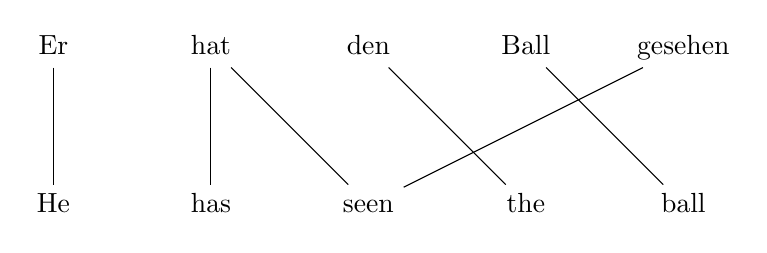
\begin{tikzpicture} [node distance = 2cm, text height=1.5ex, text depth=.25ex]
    % place nodes
    \node (Er) {Er};
    \node [right of = Er] (hat) {hat};
    \node [right of = hat] (den) {den};
    \node [right of = den] (Ball) {Ball};
    \node [right of = Ball] (gesehen) {gesehen};
    %\node [right of = gesehen] (germanDot) {.};
    \node [below of = Er] (He) {He};
    \node [right of = He] (has) {has};
    \node [right of = has] (seen) {seen};
    \node [right of = seen] (the) {the};
    \node [right of = the] (ball) {ball};
    %\node [right of = ball] (englishDot) {.};
    % draw edges
    \draw (Er) -- (He);
    \draw (hat) -- (has);
    \draw (den) -- (the);
    \draw (Ball) -- (ball);
    \draw (gesehen) -- (seen);
    %\draw (germanDot) -- (englishDot);
    % spurious alignment link
    \draw (hat) -- (seen);
  \end{tikzpicture}
  \end{center}
  \caption{German-English word-aligned sentence pair. The spurious alignment
  link between the German word \emph{hat} (\emph{has}) and the English word \emph{seen}
  prevents the phrase pair $\langle$\emph{hat}, \emph{has}$\rangle$ to be extracted from this
  sentence pair.}
  \label{fig:wordalignedSentencePairMistake}
\end{figure}
%
Intuitively, we can tell that
there is a spurious alignment link between the German
word \emph{hat} (\emph{has}) and the
English word \emph{seen}. This link will prevent the extraction of the useful
phrase pair $\langle$\emph{hat}, \emph{has}$\rangle$
from this sentence pair. However, it is
possible that the \emph{posterior probability} of this spurious link according
to the alignment model is relatively low. We hypothesise that posterior
probability information from alignment models is more reliable than the links
obtained from Viterbi alignment.

In this chapter, we use HMM alignment
models (see \autoref{sec:statisticalMachineTranslationHmmAlignmentModel}) to
generate the statistics needed to both extract rules and estimate the
translation models. We hypothesise that this tighter coupling between alignment
and translation models will provide better translation quality.

We will evaluate the grammar we obtain in two ways. First, we will assess the
grammar's ability to generate a reference translation from a source sentence.
This is determined by the type of reordering allowed by the grammar and by
the choice of translations for each source side of a rule. We will then evaluate
translation quality provided by this grammar.

Conceptually, our extraction method consists in extracting all possible phrase
pairs and hierarchical phrase pairs given a sentence pair and selecting only
those that satisfy certain statistical criteria related to alignment posterior
probabilities. For example, we can select phrase pairs that contain a link with
a high posterior probability; or we can select phrase pairs that contain a link
with a high posterior probability and that have a high phrase pair posterior
probability. The selection process determines which rules the grammar will
contain and will therefore define the ability of the grammar to generate a
reference translation given a source sentence. We can also use statistics from
alignment models to estimate translation models in a novel way. In this work, we
will use phrase pair posterior probability instead of integer counts to estimate
translation models.

\section{Related Work}
\label{sec:extractionFromPosteriorRelated}

The limitations of extracting translation rules from Viterbi alignments, i.e.
that potentially useful information from the alignment models is ignored, has
been addressed previously. \citet{venugopal-zollmann-smith-vogel:2008:AMTA}
extract rules from
$n$-best lists of alignments and $n$-best lists of syntactic parses for a
syntax-augmented hierarchical system~\citep{zollmann-venugopal:2006:WMT}.
In the alignment step, an $n$-best list of alignments $\bm{a_1}, ..., \bm{a_n}$ is
produced with posterior probabilities
$p(\bm{a_1} \mid \bm{f}, \bm{e}), ..., p(\bm{a_n} \mid \bm{f}, \bm{e})$. These
posteriors are normalised to produce probabilities
$\hat{p}(\bm{a_1}), ..., \hat{p}(\bm{a_n})$. Similarly, probabilities
$\hat{p}(\bm{\pi_1}), ..., \hat{p}(\bm{\pi_{n'}})$ are obtained
for an $n'$-best list of parses $\bm{\pi_1}, ..., \bm{\pi_{n'}}$. For each alignment
$\bm{a_i}$ and parse $\bm{\pi_j}$, syntax-augmented hierarchical rules are extracted
with a count $\hat{p}(\bm{a_i}) \, \hat{p}(\bm{\pi_j})$.

Alignment $n$-best lists have also been used to create a
structure called
\emph{weighted alignment matrix}~\citep{liu-xia-xiao-liu:2009:EMNLP}.
Probabilities $\hat{p}(\bm{a_1}), ..., \hat{p}(\bm{a_n})$
for $n$-best alignments $\bm{a_1}, ..., \bm{a_n}$ are computed
as previously~\citep{venugopal-zollmann-smith-vogel:2008:AMTA}.
Then, for each word pair $(f_j, e_i)$, the alignment link posterior
probability $p_m(j, i)$ is computed in \autoref{eq:matrixLinkPosterior}.
%
\begin{equation}
  p_m(j, i) = \sum_{k = 1}^n \hat{p}(\bm{a_k}) \delta(\bm{a_k}, i, j)
  \label{eq:matrixLinkPosterior}
\end{equation}
%
$\delta(\bm{a_k}, i, j)$ indicates whether there is a link between $i$ and
$j$ in the alignment $\bm{a_k}$. Given a sentence pair, all phrase
pairs with a maximum source length and a maximum target length that
contain a link with a posterior greater than zero are extracted. The
fractional counts assigned to these phrase pairs are computed in terms
of the link posteriors and then used to estimate the translation models
by relative frequency. The fractional count computation approximates
the posterior probability of all alignments consistent with the phrase
pair. Our method also uses link posterior probabilities
to constrain the extraction but the posteriors are computed
exactly rather than approximated. In addition, posterior probabilities
of consistent alignments is also computed exactly. Finally, our method
is also applied to hierarchical phrase-based translation.

Alignment posterior probabilities without approximation have also been
used.
For a given test set, \citet{deng-and-byrne:2008:ASLP} first extract
phrase pairs in a standard manner. Then, source phrases in the test set
that do not have any corresponding target in the list of extracted
phrase pairs are selected. For each of these source phrases, sentence
pairs where the source phrase occurs are considered. For each such
sentence pair, all target phrases in the target sentence are assigned
phrase pair posterior
probabilities (see \autoref{sec:extractionFromPosteriorsPhrasePair})
according to the
source-to-target and target-to-source alignment models, then ranked
by the geometric average of the two probabilities. The top phrase pair
is retained if its scores are above specific thresholds.
Our definition of phrase pair posterior probabilities and the procedure to compute
them are directly inspired by the work we just described. However, we do not use
the word-to-phrase HMM model but the simpler word-to-word HMM model.
In addition, our method is applied to hierarchical phrase-based grammars
rather than simpler phrase-based grammars. Finally, our grammar
extraction scheme does not consist in
first extracting a standard grammar and then augmenting the grammar with additional rules: we
modify the extraction procedure to directly extract a hierarchical
grammar from alignment link posterior probabilities
or phrase pair posterior probabilities.

\citet{kumar-och-macherey:2007:EMNLP} also use exact computation
of alignment link posteriors in a different application setting.
First, instead of using the Viterbi criterion for word alignment
reminded in \autoref{eq:viterbiCriterion},
%
\begin{equation}
  \bm{\hat{a}} = \argmax_{\bm{a}} p(\bm{f}, \bm{a} \mid \bm{e})
  \label{eq:viterbiCriterion}
\end{equation}
%
the maximum a posteriori criterion~\citep{matusov-zens-ney:2004:COLING}, shown in \autoref{eq:mapCriterion}, is used:
%
\begin{equation}
  \hat{a}_j = \argmax_{i} p(a_j = i \mid \bm{f}, \bm{e})
  \label{eq:mapCriterion}
\end{equation}
%
Then, given a parallel corpus for three languages $F$, $G$, $E$, the
link posteriors for the language pair ($F$, $E$) are computed
in terms of the posteriors for the language pair ($F$, $G$) and ($G$, $E$).
G is called a \emph{bridge} language. The motivation is that
alignments for the $F$-$G$ language pair and the $G$-$E$ language
pair may inform alignment for $F$-$E$. Multiple bridge languages are used
and produce corresponding posterior matrices. The matrices are interpolated
and alignments are extracted for each bridge language and for the
interpolation. Translation gains are obtained in system combination.

We also note approaches to tighter coupling between hierarchical phrase-based
grammars and alignments or even direct modelling of phrase alignment.
\citet{marcu-wong:2002:EMNLP} introduce a joint phrase-based model that
does not make use of word alignments. In this generative model, a sentence
pair is produced by concatenating phrase pairs, or so-called \emph{concepts}.
The authors consider a simpler model with only joint phrase pair translation
probabilities and a more complex model with translation and distortion
probabilities. The parameter are trained with an approximate version of the
expectation-maximisation algorithm~\citep{dempster-laird-rubin:1977:JRSS}.
Experiments demonstrate translation improvements over IBM Model 4.
\citet{birch-callisonburch-osborne-koehn:2006:WMT} constrain this model
in order to be able to apply it to larger parallel corpora. When searching for
a set of phrase pairs to cover a training sentence pair, phrase pairs that
are consistent with the intersection of Viterbi
alignments (see \autoref{sec:symmetrisationHeuristics}) are considered first; other
phrase pairs are considered only when the sentence pair cannot be covered entirely.
Results close to standard phrase-based models are obtained.


\citet{denero-klein:2008:ACL} prove that phrase alignment is an
NP-hard problem. Given a sentence pair $(\bm{f}, \bm{e})$, a bijective phrase
alignment $\bm{a}$ is defined as a bijective mapping between source phrases that
form a partition of $\bm{f}$ and target phrases that form a partition of
$\bm{e}$. A scoring function $\phi$ is also defined that assigns a real-valued
score to any phrase pair $\langle$source phrase, target phrase$\rangle$. The score of a
bijective phrase alignment is simply the product of the scores of its phrase pairs.
Given $(\bm{f}, \bm{e}, \phi)$, the phrase alignment optimisation problem is to find
the best scoring alignment. \citet{denero-klein:2008:ACL} show that this problem
is NP-hard by showing that the corresponding decision problem is NP-complete via
reduction of the SAT problem. We give here an indication of the size of the search
space. The number of possible source partitions is $2^{|\bm{f}| - 1}$.
Given a source partition with $K + 1$ phrases, there are $(K + 1)!$ possible
permutation of the source phrases and $2^{{|e| - 1} \choose K}$ possible target
partitions with $K+1$ phrases. In conclusion, there is little hope to solve
the phrase alignment problem exactly.

\citet{saers-wu:2009:SSST} report an
improvement on a phrase-based system where word alignment has been trained with
an inversion transduction grammar rather than IBM or HMM models.
Phrase alignment is directly modelled with an inversion transduction
grammar. The phrase alignment search space is more restrictive than
the space considered in \citet{denero-klein:2008:ACL} and the
expectation maximisation algorithm can be carried out in $O(n^6)$
where $n$ is the number of tokens in a sentence.
\citet{pauls-klein-chiang-knight:2010:NAACL} also use an
inversion transduction grammar to directly align phrases to nodes in a
string-to-tree model. Bayesian methods have also been developed to induce a
grammar directly from an unaligned parallel
corpus~\citep{blunsom-cohn-osborne:2008:NIPS,blunsom-cohn-dyer-osborne:2009:ACL}.
Finally, \citet{Cmejrek2009} extract rules directly from
bilingual chart parses of the parallel corpus without using word alignments.
We take a different approach in that we aim to start with very strong alignment
models and use them to guide grammar extraction.

Finally, some work on smoothing, which could be complementary to the approach taken
in this thesis, has been conducted to address the
shortcomings of relative frequency estimation for translation models.
\citet{foster-kuhn-johnson:2006:EMNLP} conduct an extensive series of
experiments that either replace the relative frequency estimated phrase table by
a smoothed phrase table or add the smoothed phrase table as a feature and
observe improvement in translation quality.

\section{Rule Extraction}
\label{sec:extractionFromPosteriorsExtraction}

In \autoref{sec:extractionFromPosteriorRelated}, we have reviewed approaches
that ``widen'' the translation pipeline by using alignment $n$-best lists.
We have also reviewed applications of exact computation of alignment posterior
probabilities and attempts to directly model phrase alignment. We will now
describe our grammar extraction methods, based on exact computation of
alignment posterior probabilities under an alignment model.
As in previous work~\citep{hopkins-langmead-vo:2011:WMT},
we first present a general approach that encompasses both standard methods
based on rule extraction from Viterbi alignments as well as our methods.
For clarity of presentation, we first describe our methods in the simpler case
of phrase-based rule extraction, then extend them to hierarchical phrase-based
rule extraction.

\subsection{General Framework for Rule Extraction}
\label{sec:extractionFromPosteriorsExtractionGeneralApproach}

We first describe a general method for the extraction of phrase-based rules.
An extension of this procedure for
hierarchical rules is described in
\autoref{sec:extractionFromPosteriorsExtractionDisjoint}. The algorithm is
described in \autoref{alg:generalRuleXtract}.
%
\begin{figure}
  \begin{algorithmic}[1]
    \Function{ExtractRules}{$f_1^J, e_1^I, \bm{a}$}
      \For{$1 \leq j_1 \leq j_2 \leq J$} \hypertarget{alg:line:sourcePhrase}{} \label{alg:line:sourcePhrase}
        \For{$1 \leq i_1 \leq i_2 \leq I$} \hypertarget{alg:line:targetPhrase}{} \label{alg:line:targetPhrase}
          \If{\Call{SourceConstraints}{$f_{j_1}^{j_2}$} \par
              \hskip\algorithmicindent \hskip\algorithmicindent $\land$ \Call{AlignConstraints}{$f_{j_1}^{j_2}, e_{i_1}^{i_2}, \bm{a}$} \par
              \hskip\algorithmicindent \hskip\algorithmicindent $\land$ \Call{TargetConstraints}{$e_{i_1}^{i_2}$}}
          \hypertarget{alg:line:constraints}{} \label{alg:line:constraints}
            \State{\Call{Extract}{\RT[$X$][$f_{j_1}^{j_2}$][$e_{i_1}^{i_2}$], \Call{Count}{$f_{j_1}^{j_2}, e_{i_1}^{i_2}$}}} \hypertarget{alg:line:extract}{} \label{alg:line:extract}
          \EndIf
        \EndFor
      \EndFor
    \EndFunction
  \end{algorithmic}
  \caption{General procedure for phrase-based rule extraction: both traditional
    rule extraction from Viterbi alignment and our method are instances of this
    procedure.}
  \label{alg:generalRuleXtract}
\end{figure}
%
Given a
sentence pair $(f_1^J, e_1^I)$, for each source index pair $(j_1, j_2)$
defining a source phrase $f_{j_1}^{j_2}$
(\hyperlink{alg:line:sourcePhrase}{line \ref{alg:line:sourcePhrase}}), for each
target index pair $(i_1, i_2)$ defining a target phrase $e_{i_1}^{i_2}$
(\hyperlink{alg:line:targetPhrase}{line \ref{alg:line:targetPhrase}}), if source
constraints, target constraints and
alignment constraints are satisfied
(\hyperlink{alg:line:constraints}{line \ref{alg:line:constraints}}), then the
phrase pair ($f_{j_1}^{j_2}$, $e_{i_1}^{i_2}$) is extracted with a certain
count (\hyperlink{alg:line:extract}{line \ref{alg:line:extract}}): the phrase
pair is added to the list of phrase pairs used in translation, and the count
will be used subsequently to compute translation models by relative frequency.
The purpose
of the constraints is to obtain a manageable number of rules. If we did not
impose constraints, we would extract $\frac{I (I + 1) J (J + 1)}{4}$ (not necessarily distinct) rules
for the sentence pair $(f_1^J, e_1^I)$. During
translation, the decoder would need to apply more pruning, which would
potentially lead to more search errors and a decrease in translation
quality.

We will now refine this general procedure to make it more practical and
closer to a possible implementation.
Let us call the source constraints $\mathcal{C}_S$, the alignment constraints
$\mathcal{C}_A$ and the target constraints $\mathcal{C}_T$. These are
Boolean functions used to select phrase pairs. In practice, source
constraints are checked on the source phrases before looking
at the target phrases. If source constraints are not met, then we need not
consider target phrases for that source phrase.
In addition, target phrases are only considered if they
satisfy alignment constraints with the source phrase and, if they do, we rank
them according to a certain ranking function $\mathcal{R}$. Target constraints also
depend on the ranking $\mathcal{R}$, for example we can decide to keep only a certain
number of target phrases per source phrase. When a phrase pair is extracted, it
is assigned a count which will be used to estimate the source-to-target and
target-to-source translation models. The counting function is called $\mathcal{C}$.
With this notation, we obtain the revised extraction procedure in
\autoref{alg:generalRuleXtractSpecialized}.
%
\begin{figure}
  \begin{algorithmic}[1]
    \Function{ExtractRules}{$f_1^J, e_1^I, \bm{a}$}
      \For{$1 \leq j_1 \leq j_2 \leq J$}
        \If{$\lnot \mathcal{C}_S(f_{j_1}^{j_2})$} \Comment{Source constraints}
          \State{\bf{continue}}
        \EndIf
        \State{$T \gets \emptyset$} \Comment{Sorted target phrases}
        \For{$1 \leq i_1 \leq i_2 \leq I$}
          \If{$\mathcal{C}_A(f_{j_1}^{j_2}, e_{i_1}^{i_2}, \bm{a})$} \Comment{Alignment constraints}
            \State{$T \gets T \cup e_{i_1}^{i_2}$}
          \EndIf
        \EndFor
        \State{\Call{Sort}{$T, \mathcal{R}$}} \Comment{Target phrases ranked according to $\mathcal{R}$}
        \For{$e_{i_1}^{i_2} \in T$}
          \If{$\mathcal{C}_T(e_{i_1}^{i_2}, T)$} \Comment{Target constraints}
            \State{\Call{Extract}{\RT[$X$][$f_{j_1}^{j_2}$][$e_{i_1}^{i_2}$], $\mathcal{C}(f_{j_1}^{j_2}, e_{i_1}^{i_2})$}}
          \EndIf
        \EndFor
      \EndFor
    \EndFunction
  \end{algorithmic}
  \caption{General procedure for phrase-based rule extraction. This version
  is more practical and closer to a possible implementation than the algorithm in \autoref{alg:generalRuleXtract}.
  Source phrases are first considered. Only if source constraints $\mathcal{C}_S$ are satisfied, then
  target phrases are considered. Targets that satisfy alignment constraints $\mathcal{C}_A$ with
  their
  source are ranked by $\mathcal{R}$. Finally, phrase pairs where the target
  satisfies target constraints can be extracted with a certain count $\mathcal{C}$.
  Note that the target constraints implicitly depend on the ranking of the
  targets by $\emph{R}$.}
  \label{alg:generalRuleXtractSpecialized}
\end{figure}
%
We will now describe different rule extraction strategies in terms of
the constraints $\mathcal{C}_S$, $\mathcal{C}_A$, $\mathcal{C_T}$,
the ranking function $\mathcal{R}$ and the counting function $\mathcal{C}$.

\subsection{Extraction from Viterbi Alignment Links}
\label{sec:extractionFromPosteriorsViterbi}

In this section, we describe the standard extraction procedure within
the framework introduced in
\autoref{sec:extractionFromPosteriorsExtractionGeneralApproach}.
Common practice takes a fixed set of word alignment links $\bm{L}$
and extracts
rules from this set. Alignment links $\bm{L}$ are obtained from
the alignment model $\bm{a}$ either by the Viterbi algorithm or
by maximum a posteriori
estimation~\citep{matusov-zens-ney:2004:COLING,kumar-och-macherey:2007:EMNLP}
and possibly using symmetrisation heuristics to combine links obtained
from source-to-target and target-to-source alignment
models (see \autoref{sec:symmetrisationHeuristics}). We can restate this
common approach in the framework proposed in
\autoref{sec:extractionFromPosteriorsExtractionGeneralApproach} and in
\autoref{alg:generalRuleXtractSpecialized} where constraints, ranking and
counting functions are defined as follows:
%
\begin{itemize}
  \item source constraints $\mathcal{C}_S(f_{j_1}^{j_2})$:
%
\begin{equation}
  j_2 - j_1 < s_{\text{max}}
\end{equation}
%
where $s_{\text{max}}$ is a integer threshold defined experimentally.
$s_{\text{max}}$ represents the maximum length of a source phrase.
  \item alignment constraints $\mathcal{C}_A(f_{j_1}^{j_2}, e_{i_1}^{i_2}, \bm{a})$:
%
\begin{equation}
  \Big( \forall (j,i) \in \bm{L}, j \in [j_1, j_2] \Leftrightarrow i \in [i_1,i_2] \Big) \land \Big( \bm{L} \cap [j_1, j_2] \times [i_1, i_2] \neq \emptyset \Big)
  \label{eq:consistencyConstraint}
\end{equation}
%
Alignment constraints have already been described in \autoref{sec:phrasextract} as
the conditions required for phrase pair extraction.
The first bracketed constraint requires that there be no alignment link between a
word inside the phrase pair and a word outside of it. The second
bracketed constraint
requires that
there be at least one alignment link in the phrase pair. Sometimes, an
additional constraint specifies that the boundary words in the phrase pair
should be aligned. In this work, this constraint is not present. % TODOFINAL repeat in background ?
A phrase pair that satisfies \autoref{eq:consistencyConstraint} is said
to be \emph{consistent} with the alignment (see \autoref{sec:phrasextract}).
  \item target constraints $\mathcal{C}_T(e_{i_1}^{i_2}, T)$: no constraint is
    imposed in this work. Target constraints based on length may be imposed
    depending on the implementation.
  \item ranking and counting functions:
%
\begin{equation}
  \mathcal{R}(f_{j_1}^{j_2},e_{i_1}^{i_2}) = \mathcal{C}(f_{j_1}^{j_2},e_{i_1}^{i_2}) = 1
\end{equation}
\end{itemize}
%
The above constraints, ranking and counting functions define the standard
approach to grammar extraction.
In the next sections, we depart from this approach and apply novel functions
to rank and count target-side translations according to their quality in the
context of each parallel sentence, as defined by the word alignment models. We
also depart from common practice in that we do not use a set of links as
alignment constraints. We thus have better control over the number of extracted
rules as well as the relative frequency estimates of the source-to-target and
target-to-source translation models.

\subsection[Extraction from Posteriors Probabilities over Alignment Links]{Extraction from Posteriors Probabilities over \\ Alignment Links}
\label{sec:extractionFromPosteriorsLink}

%We now consider the hidden random variable $\bm{a}$ that models the
%alignment process.
For presentation, we only consider source-to-target
alignment models: the random variable $\bm{a}$ that models the alignment
process
takes values in functions from source
word positions to target word positions. However, it it possible to apply
our method with any directional alignment model.
We will use the link
posterior probability $p(a_j = i \mid f_1^J, e_1^I)$ to guide
rule extraction. This statistic expresses how likely it is that
a word $f_j$ in source position $j$ and a word $e_i$ in
target position $i$ are aligned given the sentence pair $(f_1^J,e_1^I)$.
The link posterior probability can be computed efficiently for
Model 1, Model 2 and HMM. In our experiments, we only use the HMM model
to compute link posteriors but comparisons between link posteriors obtained
from various models may be interesting in the future. We will derive
a closed form solution for these models to compute the link posterior
probability.
Applying the definition of conditional
probability, we obtain the general form of the link posterior probability in
\autoref{eq:linkposdef}.
%
\begin{equation} \label{eq:linkposdef}
  p(a_{j_0} = i_0 \mid f_1^J, e_1^I) = \frac{p(a_{j_0}=i_0,f_1^J \mid e_1^I)}{p(f_1^J \mid e_1^I)}
\end{equation}
%
Using \autoref{eq:linkposdef}, we will now derive the link posterior probability
$p_{M_1}(a_{j_0} = i_0 \mid f_1^J, e_1^I)$ for Model 1,
$p_{M_2}(a_{j_0} = i_0 \mid f_1^J, e_1^I)$ for Model 2 and
$p_{\text{HMM}}(a_{j_0} = i_0 \mid f_1^J, e_1^I)$ for the HMM model.

\subsubsection{Link Posterior Probability for Model 1}

Let us derive $p_{M_1}(a_{j_0} = i_0 \mid f_1^J, e_1^I)$,
the link posterior probability under Model 1. We use the notation
from~\citep{brown-dellapietra-dellapietra-mercer-1993}, where $t$ is
the word-to-word translation table and $\varepsilon$ is a constant. We compute the
numerator from
\autoref{eq:linkposdef} by marginalising over all possible alignments and
inverting sum and product signs to obtain \autoref{eq:linkposM1Numerator}:
%
\begin{align}
  & p_{M_1}(a_{j_0}=i_0,f_1^J \mid e_1^I) \nonumber \\
  &= \sum_{a_1 = 0}^{I} ... \sum_{a_{j_0-1} = 0}^{I} \sum_{a_{j_0+1} = 0}^{I} ... \sum_{a_J = 0}^{I} p_{M_1}(a_1 ... a_{j_0-1} i_0 a_{j_0+1} ... a_J,f_1^J \mid e_1^I) \nonumber \\
  &= \sum_{a_1 = 0}^{I} ... \sum_{a_{j_0-1} = 0}^{I} \sum_{a_{j_0+1} = 0}^{I} ... \sum_{a_J = 0}^{I} \frac{\varepsilon}{(1+I)^J} t(f_{j_0} \mid e_{i_0}) \prod_{\substack{j = 1 \\ j \neq j_0}}^J t(f_j \mid e_{a_j}) \nonumber \\
  &= \frac{\varepsilon}{(1+I)^J} t(f_{j_0} \mid e_{i_0}) \prod_{\substack{j = 1 \\ j \neq j_0}}^J \sum_{i=0}^I t(f_j \mid e_i) \label{eq:linkposM1Numerator}
\end{align}
%
We compute the denominator from \autoref{eq:linkposdef}
similarly (see Equation (15)
in~\citep{brown-dellapietra-dellapietra-mercer-1993}) and obtain
\autoref{eq:linkposM1Denominator}:
%
\begin{equation} \label{eq:linkposM1Denominator}
  p_{M_1}(f_1^J \mid e_1^I) = \frac{\varepsilon}{(1+I)^J} \prod_{j=1}^J \sum_{i=0}^I t(f_j \mid e_i)
\end{equation}
%
After simplification, we obtain \autoref{eq:linkposM1} from
\autoref{eq:linkposM1Numerator} and \autoref{eq:linkposM1Denominator}:
%
\begin{equation} \label{eq:linkposM1}
  p_{M_1}(a_{j_0} = i_0 \mid f_1^J, e_1^I) = \frac{t(f_{j_0}|e_{i_0})}{\sum_{i=0}^I t(f_{j_0}|e_i)}
\end{equation}
%

\subsubsection{Link Posterior Probability for Model 2}
We apply the same method to compute $p_{M_2}(a_{j_0} = i_0 \mid f_1^J, e_1^I)$, the
link posterior probability for Model 2. We also use
notation from~\citep{brown-dellapietra-dellapietra-mercer-1993} but
we replace the notation for the alignment probability $a(i \mid j, J, I)$
by $p_a(i \mid j, J, I)$ for clarity.
We compute the numerator from \autoref{eq:linkposdef} in
\autoref{eq:linkposM2Numerator}:
%
\begin{align}
  & p_{M_2}(a_{j_0}=i_0,f_1^J \mid e_1^I) \nonumber \\
  &= \sum_{a_1 = 0}^{I} ... \sum_{a_{j_0-1} = 0}^{I} \sum_{a_{j_0+1} = 0}^{I} ... \sum_{a_J = 0}^{I} p_{M_2}(a_1 ... a_{j_0-1} i_0 a_{j_0+1} ... a_J,f_1^J \mid e_1^I) \nonumber \\
  &= \sum_{a_1 = 0}^{I} ... \sum_{a_{j_0-1} = 0}^{I} \sum_{a_{j_0+1} = 0}^{I} ... \sum_{a_J = 0}^{I} \varepsilon \ p_a(i_0 \mid j_0, J, I) \ t(f_{j_0} \mid e_{i_0}) \nonumber \\
  & \; \; \qquad \qquad \qquad \qquad \qquad \qquad \prod_{\substack{j = 1 \\ j \neq j_0}}^J p_a(a_j \mid j, J, I) \ t(f_j \mid e_{a_j}) \nonumber \\
  &= \varepsilon \ p_a(i_0 \mid j_0, J, I) \ t(f_{j_0} \mid e_{i_0}) \prod_{\substack{j = 1 \\ j \neq j_0}}^J \sum_{i=0}^I p_a(i \mid j, J, I) \ t(f_j \mid e_i) \label{eq:linkposM2Numerator}
\end{align}
%
We compute the denominator from \autoref{eq:linkposdef} similarly and obtain
\autoref{eq:linkposM2Denominator}:
%
\begin{equation} \label{eq:linkposM2Denominator}
  p_{M_2}(f_1^J \mid e_1^I) = \varepsilon \ \prod_{j=1}^J \sum_{i=0}^I p_a(i \mid j, J, I) \ t(f_j \mid e_i)
\end{equation}
%
After simplification, we obtain \autoref{eq:linkposM2} from
\autoref{eq:linkposM2Numerator} and \autoref{eq:linkposM2Denominator}.
%
\begin{equation} \label{eq:linkposM2}
  p_{M_2}(a_{j_0} = i_0 \mid f_1^J, e_1^I) = \frac{p_a(i_0 \mid j_0, J, I) \ t(f_{j_0} \mid e_{i_0})}{\sum_{i=0}^I p_a(i \mid j_0, J, I) \ t(f_{j_0} \mid e_i)}
\end{equation}
%

\subsubsection{Link Posterior Probability for the HMM Model}
\label{sec:linkPosteriorHMM}
We now derive $p_{\text{HMM}}(a_{j_0} = i_0 | f_1^J, e_1^I)$, the link posterior
probability for the HMM
model~\citep{vogel-ney-tillmann,rabiner:1989:IEEE}. These derivations
are standard once we realise that the observed sequence is the source
sentence $f_1^J$, the hidden sequence is $a_1^J$ and that in addition
to standard presentations of HMM, all probabilities are conditioned on
the target sentence $e_1^I$.
We compute the numerator from \autoref{eq:linkposdef} in
\autoref{eq:linkposHMMNumerator}:
%
\begin{align}
  p_{\text{HMM}}(a_{j_0} = i_0, f_1^J \mid e_1^I) &= p_{\text{HMM}}(a_{j_0} = i_0, f_1^{j_0}, f_{j_0 + 1}^J \mid e_1^I) \nonumber \\
                                               &= p_{\text{HMM}}(f_{j_0 + 1}^J \mid a_{j_0} = i_0, f_1^{j_0}, e_1^I) \ p_{\text{HMM}}(a_{j_0} = i_0, f_1^{j_0} \mid e_1^I) \nonumber \\
                                               &= p_{\text{HMM}}(f_{j_0 + 1}^J \mid a_{j_0} = i_0, e_1^I) \ p_{\text{HMM}}(a_{j_0} = i_0, f_1^{j_0} \mid e_1^I) \nonumber \\
                                               &= \beta_{j_0}(i_0) \ \alpha_{j_0}(i_0) \label{eq:linkposHMMNumerator}
\end{align}
%
where $\beta_{j_0}(i_0)$ and $\alpha_{j_0}(i_0)$ are respectively
the backward and forward HMM probabilities defined in \autoref{eq:backwardForward}:
%
\begin{equation}
  \begin{split}
    \beta_{j}(i)  &= p_{\text{HMM}}(f_{j + 1}^J \mid a_{j} = i, e_1^I) \\
    \alpha_{j}(i) &= p_{\text{HMM}}(a_{j} = i, f_1^{j} \mid e_1^I)
  \end{split}
  \label{eq:backwardForward}
\end{equation}
%
The forward and backward probabilities can be computed recursively as
shown in \autoref{eq:forwardRecursion} and \autoref{eq:backwardRecursion}:
%
\begin{align}
  \alpha_{j}(i) &= p_{\text{HMM}}(a_{j} = i, f_1^{j} \mid e_1^I) \nonumber \\
                &= \sum_{k = 0}^I p_{\text{HMM}}(a_{j} = i, a_{j - 1} = k, f_1^{j - 1}, f_j \mid e_1^I) \nonumber \\
                &= \sum_{k = 0}^I p_{\text{HMM}}(f_j \mid a_j = i, a_{j - 1} = k, f_1^{j-1}, e_1^I) \ p_{\text{HMM}}(a_{j} = i, a_{j - 1} = k, f_1^{j - 1} \mid e_1^I) \nonumber \\
                &= \sum_{k = 0}^I p_{\text{HMM}}(f_j \mid e_i) \ p_{\text{HMM}}(a_{j} = i \mid a_{j - 1} = k, f_1^{j - 1}, e_1^I) \ p_{\text{HMM}}(a_{j - 1} = k, f_1^{j - 1} \mid e_1^I) \nonumber \\
                &= \sum_{k = 0}^I p_{\text{HMM}}(f_j \mid e_i) \ p_{\text{HMM}}(a_{j} = i \mid a_{j - 1} = k, I) \ \alpha_{j - 1}(k) \label{eq:forwardRecursion} \\
  \beta_{j}(i)  &= p_{\text{HMM}}(f_{j + 1}^J \mid a_{j} = i, e_1^I) \nonumber \\
                &= \sum_{k = 0}^I p_{\text{HMM}}(f_{j+2}^J, a_{j + 1} = k, f_{j + 1} \mid a_j = i, e_1^I) \nonumber \\
                &= \sum_{k = 0}^I p_{\text{HMM}}(f_{j+2}^J \mid a_{j + 1} = k, f_{j + 1}, a_j = i, e_1^I) \ p_{\text{HMM}}(a_{j + 1} = k, f_{j + 1} \mid a_j = i, e_1^I) \nonumber \\
                &= \sum_{k = 0}^I p_{\text{HMM}}(f_{j+2}^J \mid a_{j + 1} = k, e_1^I) \ p_{\text{HMM}}(f_{j + 1} \mid a_{j + 1} = k, a_j = i, e_1^I) \nonumber \\
                & p_{\text{HMM}}(a_{j + 1} = k \mid a_j = i, e_1^I) \nonumber \\
                &= \sum_{k = 0}^I \beta_{j + 1}(k) \ p_{\text{HMM}}(f_{j + 1} \mid e_k) \ p_{\text{HMM}}(a_{j + 1} = k \mid a_j = i, I) \label{eq:backwardRecursion}
\end{align}
%
The denominator from \autoref{eq:linkposdef} is computed in
\autoref{eq:linkposHMMDenominator}:
%
\begin{align}
  p_{\text{HMM}}(f_1^J \mid e_1^I) &= \sum_{k = 0}^I p_{\text{HMM}}(a_J = k, f_1^J \mid e_1^I) \nonumber \\
                                &= \sum_{k = 0}^I \alpha_J(k) \label{eq:linkposHMMDenominator}
\end{align}
%
%
%We now derive the link posterior probability for the WPHMM Model.
%TODONEVER(should refer here to a background section for notation, etc.)
% TODONEVER: link posteriors for WPHMM and phrase pair posteriors
%

We will use the link posterior probabilities under the HMM model
in order to define constraints, ranking and counting functions.

\subsubsection{Constraints, Ranking and Counting Functions from HMM Link Posterior Probabilities}

We use HMM link posterior probabilities computed in \autoref{sec:linkPosteriorHMM}
in order to define constraints, ranking and counting functions:
%
\begin{itemize}
  \item source constraints $\mathcal{C}_S(f_{j_1}^{j_2})$:
%
\begin{equation}
  j_2 - j_1  < s_{\text{max}}
\end{equation}
%
This is the same constraint as defined for standard Viterbi extraction in
\autoref{sec:extractionFromPosteriorsViterbi}.
  \item alignment constraints $\mathcal{C}_A(f_{j_1}^{j_2}, e_{i_1}^{i_2}, \bm{a})$:
%
\begin{align}
 & \exists (j,i) \in [j_1,j_2] \times [i_1,i_2], p(a_j = i \mid f_1^J,e_1^I) > \lambda \label{eq:firstAlignmentConstraintHmmLinkPosterior} \\
 & \forall (j,i) \in [1, J] \times [1, I] \cap \{(j,i): p(a_j = i \mid f_1^J,e_1^I) > \lambda\} \label{eq:secondAlignmentConstraintHmmLinkPosterior} \\
 & \hspace{3em} j \in [j_1, j_2] \Leftrightarrow i \in [i_1, i_2] \nonumber
\end{align}
%
where $\lambda$ is a threshold defined experimentally. Intuitively,
$\lambda$ is a high link posterior probability.
The first constraint (\autoref{eq:firstAlignmentConstraintHmmLinkPosterior}) means that we require at least one link with a
high posterior probability in the phrase pair considered. The second
constraint (\autoref{eq:secondAlignmentConstraintHmmLinkPosterior}) means that there should be no link with a high posterior probability
that be inconsistent with the phrase pair. Note that these constraints are
identical to the Viterbi alignment constraints defined
in \autoref{sec:extractionFromPosteriorsViterbi} if we choose $\bm{L}$ to be the
set of all links with high posterior defined in \autoref{eq:linksWithHighPosterior}:
%
\begin{equation}
  \bm{L} = \{(j, i) \in [1, J] \times [1, I]: p(a_j = i \mid f_1^J,e_1^I) > \lambda\}
  \label{eq:linksWithHighPosterior}
\end{equation}
%
Also note that the second
constraint does not consider links to the null
word (see \autoref{sec:StatisticalMachineTranslationWordAlignment}) relevant.
This is because we do not need to include the null word
in a translation rule.
  \item target constraints $\mathcal{C}_T(e_{i_1}^{i_2}, T)$: we pick the
    first $k$ translation candidates according to the ranking
    function $\mathcal{R}$.
  \item ranking function:
%
\begin{equation} \label{eq:linkPosRanking}
  \mathcal{R}(f_{j_1}^{j_2},e_{i_1}^{i_2}) = \prod_{j=j_1}^{j_2} \sum_{i=i_1}^{i_2} \frac{p(a_j = i \mid f_1^J,e_1^I)}{i_2-i_1+1}
\end{equation}
%
This ranking function is very similar to the score used for lexical features
described in \autoref{sec:features}. Here,
we use link posteriors instead of Model 1 translation probabilities. This
function favours short target phrases, therefore we do not use it as a counting
function. Preliminary experiments found that this function is not appropriate for
counting rules and that it gives poor results. We therefore use the same counting
function as in standard practice described in
\autoref{sec:extractionFromPosteriorsViterbi}.
  \item counting function:
%
\begin{equation}
  \mathcal{C}(f_{j_1}^{j_2},e_{i_1}^{i_2}) = 1
\end{equation}
%
\end{itemize}

We have described rule extraction from alignment link posterior
probabilities. Next, we will describe rule extraction from alignment
posterior probabilities over phrase pairs. This method will use the
same source constraints, alignment constraints and target constraints
but different ranking and counting functions.

\subsection{Extraction from Posteriors over Phrase Pairs}
\label{sec:extractionFromPosteriorsPhrasePair}

In the previous section, we defined and gave closed form solutions to
alignment link posterior probabilities for Model 1, Model 2 and the HMM model.
We can also define alignment posterior probabilities over phrase pairs. Let us
consider the phrase pair $\langle f_{j_1}^{j_2}, e_{i_1}^{i_2} \rangle$ in the
sentence pair $(f_1^J, e_1^I)$. In
\autoref{eq:alignmentConsistentDefinition}, we define
$A(j_1, j_2; i_1, i_2)$, the set of alignments that have no links between
inside the phrase pair and outside the phrase pair:
%
\begin{equation}
  A(j_1, j_2;i_1, i_2) = \{a_1^J : a_j \in [i_1, i_2] \Leftrightarrow j \in [j_1,j_2] \}
  \label{eq:alignmentConsistentDefinition}
\end{equation}
%
Alignments in $A(j_1, j_2;i_1, i_2)$ satisfy the consistency constraint
defined in \autoref{eq:consistencyConstraint}
but do not require a link in $[j_1, j_2] \times [i_1, i_2]$.
The posterior probability of these alignments given the sentence
pair is defined in \autoref{eq:phrasePairPosteriorDefinition}:
%
\begin{equation}
  \begin{split}
  p(A(j_1, j_2; i_1, i_2) \mid e_1^I, f_1^J) &= \frac{p(f_1^J, A(j_1, j_2; i_1, i_2) \mid e_1^I)}{p(f_1^J \mid e_1^I)} \\
                                          &= \frac{\sum_{a_1^J \in A(j_1, j_2; i_1, i_2)} p(f_1^J,a_1^J \mid e_1^I)}{\sum_{a_1^J} p(f_1^J,a_1^J \mid e_1^I)}
  \end{split}
  \label{eq:phrasePairPosteriorDefinition}
\end{equation}
%
We call this quantity the \emph{phrase pair posterior probability}.
We will now derive formula for the phrase pair posterior probability in the
case of Model 1, Model 2 and the HMM Model. Again, experiments only use phrase pair
posteriors computed from the HMM model, but comparing those with the posteriors
obtained from Model 1 and Model 2 may be interesting for future research.

\subsubsection{Phrase Pair Posterior Probability for Model 1}

Let us first define $J_{\text{in}}$, $J_{\text{out}}$, $I_{\text{in}}$ and
$I_{\text{out}}$ in \autoref{eq:iInsideOutside} for a set of indices
$i_1$, $i_2$, $j_1$, $j_2$:
%
\begin{equation}
\begin{split}
  J_{\text{in}} &= [j_1, j_2] \\
  J_{\text{out}} &= [1,J] \setminus J_{\text{in}} \\
  I_{\text{in}} &= [i_1, i_2] \\
  I_{\text{out}} &= [0, I] \setminus I_{\text{in}}
\end{split}
\label{eq:iInsideOutside}
\end{equation}
%
For Model 1, the numerator from \autoref{eq:phrasePairPosteriorDefinition} is
obtained in \autoref{eq:phrasePairPosteriorModel1Numerator}:
%
\begin{align}
  & \sum_{a_1^J \in A(j_1, j_2; i_1, i_2)} p_{M_1}(f_1^J, a_1^J \mid e_1^I) \nonumber \\
  &= \sum_{a_1 \in I_{\text{out}}} ... \sum_{a_{j_1-1} \in I_{\text{out}}} \sum_{a_{j_1} \in I_{\text{in}}} ... \sum_{a_{j_2} \in I_{\text{in}}} \sum_{a_{j_2 + 1} \in I_{\text{out}}} ... \sum_{a_J \in I_{\text{out}}} p_{M_1}(a_1^J, f_1^J \mid e_1^I) \nonumber \\
  &= \sum_{a_1 \in I_{\text{out}}} ... \sum_{a_{j_1-1} \in I_{\text{out}}} \sum_{a_{j_1} \in I_{\text{in}}} ... \sum_{a_{j_2} \in I_{\text{in}}} \sum_{a_{j_2 + 1} \in I_{\text{out}}} ... \sum_{a_J \in I_{\text{out}}} \frac{\varepsilon}{(1+I)^J} \prod_{j = 1}^J t(f_j \mid e_{a_j}) \nonumber \\
  &= \frac{\varepsilon}{(1+I)^J} \ \left( \prod_{j \in J_{\text{out}}} \sum_{i \in I_{\text{out}}} t(f_j \mid e_i) \right) \ \left( \prod_{j \in J_{\text{in}}} \sum_{i \in I_{\text{in}}} t(f_j \mid e_i) \right)
  \label{eq:phrasePairPosteriorModel1Numerator}
\end{align}
%
The denominator from \autoref{eq:phrasePairPosteriorDefinition} has already been
computed in \autoref{eq:linkposM1Denominator}.
Simplifying \autoref{eq:phrasePairPosteriorModel1Numerator} and
\autoref{eq:linkposM1Denominator}, we obtain
\autoref{eq:phrasePairPosteriorModel1}:
%
\begin{align}
  & p_{M_1}(A(j_1, j_2; i_1, i_2) \mid e_1^I, f_1^J) \nonumber \\
  &= \left( \prod_{j \in J_{\text{out}}} \sum_{i \in I_{\text{out}}} \frac{t(f_j \mid e_i)}{\sum_{i' = 0}^I t(f_{j} \mid e_{i'})} \right)  \left( \prod_{j \in J_{\text{in}}} \sum_{i \in I_{\text{in}}} \frac{t(f_j \mid e_i)}{\sum_{i' = 0}^I t(f_{j} \mid e_{i'})} \right) \nonumber \\
  &= \left( \prod_{j \in J_{\text{out}}} \sum_{i \in I_{\text{out}}} p_{M_1}(a_j = i \mid f_1^J, e_1^I) \right) \left( \prod_{j \in J_{\text{in}}} \sum_{i \in I_{\text{in}}} p_{M_1}(a_j = i \mid f_1^J, e_1^I) \right)
  \label{eq:phrasePairPosteriorModel1}
\end{align}
%

\subsubsection{Phrase Pair Posterior Probability for Model 2}

To avoid repetition, we skip the derivation which is analogous to
the derivation for Model 1. We obtain the phrase pair posterior in
\autoref{eq:phrasePairPosteriorModel2}:
%
\begin{align}
  & p_{M_2}(A(j_1, j_2; i_1, i_2) \mid e_1^I, f_1^J) \nonumber \\
  &= \left( \prod_{j \in J_{\text{out}}} \sum_{i \in I_{\text{out}}} p_{M_2}(a_j = i \mid f_1^J, e_1^I) \right) \left( \prod_{j \in J_{\text{in}}} \sum_{i \in I_{\text{in}}} p_{M_2}(a_j = i \mid f_1^J, e_1^I) \right)
  \label{eq:phrasePairPosteriorModel2}
\end{align}
%

\subsubsection{Phrase Pair Posterior Probability for HMM}

Let us now compute the phrase pair posterior probability for the HMM model. The
denominator from \autoref{eq:phrasePairPosteriorDefinition} can be computed using
the forward algorithm while the numerator can be computed using a modified
forward algorithm~\citep{deng:2005:PHD}. Let us define $\tilde{\alpha}_j(i)$, the
modified forward probability in \autoref{eq:modifiedForwardProbabilityDefinition}:
%
\begin{equation}
  \tilde{\alpha}_j(i) = p_{\text{HMM}}(A(j_1,j_2;i_1,i_2), f_1^j, a_j=i \mid e_1^I)
  \label{eq:modifiedForwardProbabilityDefinition}
\end{equation}
%
The numerator from \autoref{eq:phrasePairPosteriorDefinition} can be computed
in \autoref{eq:phrasePairPosteriorHMMNumerator}:
%
\begin{equation}
  p(A(j_1, j_2; i_1, i_2), f_1^J \mid e_1^I) = \sum_{i=0}^I \tilde{\alpha}_J(i)
  \label{eq:phrasePairPosteriorHMMNumerator}
\end{equation}
%
The denominator from \autoref{eq:phrasePairPosteriorDefinition} can be computed
using the regular forward probability in
\autoref{eq:phrasePairPosteriorHMMDenominator}:
%
\begin{equation}
  p(f_1^J \mid e_1^I) = \sum_{i=0}^I \alpha_J(i)
  \label{eq:phrasePairPosteriorHMMDenominator}
\end{equation}
%
Like the regular forward probability, the modified forward probability can also
be computed recursively. We can also write the modified forward probability as
in \autoref{eq:rewriteModifiedForwardProbability}:
%
\begin{equation}
  \begin{split}
  \tilde{\alpha}_j(i) &= p_{\text{HMM}}(A(j_1,j_2;i_1,i_2), f_1^j, a_j=i \mid e_1^I) \\
                      &= \sum_{a_1^{j} \in A(j_1,j_2;i_1,i_2)} p_{\text{HMM}}(a_1^{j-1}, f_1^j, a_j=i \mid e_1^I) \\
                      &= \sum_{\substack{a_1^{j} \in A(j_1,j_2;i_1,i_2) \\ a_j=i}} p_{\text{HMM}}(a_1^{j-1}, f_1^j, a_j=i \mid e_1^I)
  \end{split}
  \label{eq:rewriteModifiedForwardProbability}
\end{equation}
%
The computation of $\tilde{\alpha}_j(i)$ is by a constrained forward algorithm where
the constraint is given in \autoref{eq:modifiedForwardConstraints}. This is because
an alignment in $A(j_1,j_2;i_1,i_2)$  cannot have a link from inside the phrase
pair to outside the phrase pair (see \autoref{eq:alignmentConsistentDefinition}):
%
\begin{equation}
  \forall (j, i) \in J_{\text{out}} \times I_{\text{in}} \cup J_{\text{in}} \times I_{\text{out}}, \tilde \alpha_j(i) = 0
  \label{eq:modifiedForwardConstraints}
\end{equation}
%
For a link $(j, i) \in J_{\text{out}} \times I_{\text{out}} \cup J_{\text{in}} \times I_{\text{in}}$ that satisfies the constraint from
\autoref{eq:modifiedForwardConstraints}, we can derive the modified
forward probability in \autoref{eq:modifiedForwardRecursion}:
%
\begin{align}
  \tilde{\alpha}_j(i) &= p_{\text{HMM}}(A(j_1, j_2; i_1, i_2), f_1^j, a_j=i \mid e_1^I) \nonumber \\
                      &= \sum_{a_1^{j-1} \in A(j_1, j_2; i_1, i_2)}
                         p_{\text{HMM}}(f_j, f_1^{j-1},  a_j=i, a_1^{j-1} \mid e_1^I) \nonumber \\
                      &= \sum_{a_1^{j-1} \in A(j_1, j_2; i_1, i_2)}
                         p_{\text{HMM}}(f_j \mid f_1^{j-1},  a_j=i, a_1^{j-1}, e_1^I) \times \nonumber \\
                      & \hspace{7.7em} p_{\text{HMM}}(a_j=i \mid f_1^{j-1}, a_1^{j-1}, e_1^I) \times \nonumber \\
                      & \hspace{7.7em} p_{\text{HMM}}(f_1^{j-1}, a_1^{j-1} \mid e_1^I) \nonumber \\
                      &= p_{\text{HMM}}( f_j \mid e_i ) 
                         \sum_{a_1^{j-1} \in A(j_1, j_2; i_1, i_2)}
                         p_{\text{HMM}}(a_j=i \mid a_{j-1}, I) \
                         p_{\text{HMM}}(f_1^{j-1},  a_1^{j-1} \mid e_1^I) \nonumber \\
                      &= p_{\text{HMM}}(f_j \mid e_i) \
                         \sum_{k=0}^I \sum_{\substack{a_1^{j-1} \in A(j_1, j_2; i_1, i_2) \\ a_{j-1} = k}}
                         p_{\text{HMM}}(a_j=i \mid a_{j-1} = k, I) \nonumber \\
                      & \hspace{15.2em} p_{\text{HMM}}(f_1^{j-1},  a_{j-1} = k,  a_1^{j-2} \mid e_1^I) \nonumber \\
                      &= p_{\text{HMM}}(f_j \mid e_i) \
                         \sum_{k = 0}^I
                         p_{\text{HMM}}(a_j = i \mid a_{j-1} = k, I) \nonumber \\
                      & \hspace{4.7em} \sum_{\substack{a_1^{j-1} \in A(j_1, j_2; i_1, i_2) \\ a_{j-1} = k}}
                         p_{\text{HMM}}(f_1^{j-1},  a_{j-1} = k,  a_1^{j-2} \mid e_1^I) \nonumber \\
                      &= p_{\text{HMM}}(f_j \mid e_i) \
                         \sum_{k = 0}^I
                         p_{\text{HMM}}(a_j=i \mid a_{j-1} = k, I) \; \tilde \alpha_{j-1}(k)
                         \label{eq:modifiedForwardRecursion}
\end{align}
%
We will use the phrase pair posterior probabilities under the HMM model
in order to define ranking and counting functions.

\subsubsection{Constraints, Ranking and Counting Functions from HMM Link and Phrase Posterior Probabilities}

In order to keep the size of the rule set manageable, we use
the same source constraints, alignment constraints and target constraints
as for link posterior extraction defined in
\autoref{sec:extractionFromPosteriorsLink}.
We use the phrase pair posterior probabilities under the HMM model both for ranking
and scoring
extracted rules. This approach assigns a fractional count to each extracted
rule, which allows finer estimation of the source-to-target and target-to-source
translation models.  The ranking and counting functions
are defined in \autoref{eq:rankingCountingPhrasePairExtraction}:
%
\begin{equation}
  \mathcal{R}(f_{j_1}^{j_2},e_{i_1}^{i_2}) = \mathcal{C}(f_{j_1}^{j_2},e_{i_1}^{i_2}) = p_{\text{HMM}}(A(j_1, j_2; i_1, i_2) \mid f_1^j, e_1^J)
  \label{eq:rankingCountingPhrasePairExtraction}
\end{equation}

Under the framework described in
\autoref{sec:extractionFromPosteriorsExtractionGeneralApproach}, we have
described standard rule extraction from Viterbi alignments and two novel
approaches to rule extraction based on link posterior probabilities and
phrase pair posterior probabilities. In order to expose concepts with more
clarity, we have restricted the presentation
to the extraction of phrase based rules as opposed to hierarchical rules.
We will now show how to generalise the techniques presented so far to
the extraction of hierarchical rules.

\subsection{Hierarchical Rule Extraction}
\label{sec:extractionFromPosteriorsExtractionDisjoint}

In this section, we extend the techniques presented so far to hierarchical
rule extraction. In order to avoid repetition, we describe these
techniques for the rule pattern
$\langle w X w, w X w \rangle$
only (see \autoref{sec:constraintsOnHierarhicalGrammars} for the
definition of patterns). We first rewrite the algorithm in
\autoref{alg:generalRuleXtractSpecialized} into the algorithm in
\autoref{alg:generalRuleXtractSpecializedHierarchical} for this pattern.
%
\begin{figure}
  \begin{algorithmic}[1]
    \Function{ExtractRules}{$f_1^J, e_1^I, \bm{a}$}
      \For{$1 \leq j_1 \leq j_2 < j_3 \leq j_4 \leq J$}
        \If{$\lnot \mathcal{C}_S(f_{j_1}^{j_2} X f_{j_3}^{j_4})$} \Comment{Source constraints}
          \State{\bf{continue}}
        \EndIf
        \State{$T \gets \emptyset$} \Comment{Sorted hierarchical target phrases}
        \For{$1 \leq i_1 \leq i_2 < i_3 \leq i_4 \leq I$}
          \If{$\mathcal{C}_A(f_{j_1}^{j_2} X f_{j_3}^{j_4}, e_{i_1}^{i_2} X e_{i_3}^{i_4}, \bm{a})$} \Comment{Alignment constraints}
            \State{$T \gets T \cup e_{i_1}^{i_2} X e_{i_3}^{i_4}$}
          \EndIf
        \EndFor
        \State{\Call{Sort}{$T, \mathcal{R}$}} \Comment{Hierarchical target phrases ranked according to $\mathcal{R}$}
        \For{$e_{i_1}^{i_2} X e_{i_3}^{i_4} \in T$}
          \If{$\mathcal{C}_T(e_{i_1}^{i_2} X e_{i_3}^{i_4}, T)$} \Comment{Target constraints}
            \State{\Call{Extract}{\RT[$X$][$f_{j_1}^{j_2} X f_{j_3}^{j_4}$][$e_{i_1}^{i_2} X e_{i_3}^{i_4}$], $\mathcal{C}(f_{j_1}^{j_2} X f_{j_3}^{j_4}, e_{i_1}^{i_2} X e_{i_3}^{i_4})$}}
          \EndIf
        \EndFor
      \EndFor
    \EndFunction
  \end{algorithmic}
  \caption{General procedure for hierarchical phrase-based rule extraction. The procedure is presented for the pattern $\langle w X w, w X w \rangle$ only. This algorithm is
  analogous to the algorithm used to extract phrase-based rules and presented
  in \autoref{alg:generalRuleXtractSpecialized}.}
  \label{alg:generalRuleXtractSpecializedHierarchical}
\end{figure}
%
We will now describe constraints, counting and ranking function for
standard Viterbi extraction and for extraction from alignment posteriors.

\subsubsection{Hierarchical Rule Extraction from Viterbi Alignment Links}

We now describe the constraints, ranking and counting functions for
hierarchical rule extraction from Viterbi alignments:
%
\begin{itemize}
  \item source constraints $\mathcal{C}_S(f_{j_1}^{j_2} X f_{j_3}^{j_4})$:
%
\begin{equation}
  \begin{split}
    (j_2 - j_1 + 1) + 1 + (j_4 - j_3 + 1) &\leq s_{\text{max elements}} \\
    j_2 - j_1 &< s_{\text{max terminals}} \\
    j_4 - j_3 &< s_{\text{max terminals}} \\
    \text{span}(X) &\leq s_\text{max NT}
  \end{split}
  \label{eq:sourceConstraintsHiero}
\end{equation}
%
We remind definitions introduced
in \autoref{sec:hfileForHiero} for the thresholds in
\autoref{eq:sourceConstraintsHiero}.
$s_{\text{max elements}}$ is the maximum number of terminals and nonterminals
in the source. $s_{\text{max terminals}}$ is the maximum number of consecutive
terminals in the source. $s_{\text{max NT}}$ is the maximum \emph{span}
for a nonterminal, i.e. the maximum number of
terminals covered by a nonterminal. These thresholds are defined
experimentally.
  \item alignment constraints $\mathcal{C}_A(f_{j_1}^{j_2} X f_{j_3}^{j_4}, e_{i_1}^{i_2} X e_{i_3}^{i_4}, \bm{a})$:
\begin{equation}
\begin{split}
  & \forall (j,i) \in \bm{L}, j \in [j_1, j_4] \Leftrightarrow i \in [i_1,i_4] \\
  & \bm{L} \cap [j_1, j_4] \times [i_1, i_4] \neq \emptyset \\
  & \forall (j,i) \in \bm{L}, j \in (j_2, j_3) \Leftrightarrow i \in (i_2, i_3) \\
  & \bm{L} \cap \{j_2 + 1\} \times (i_2, i_3) \neq \emptyset \\
  & \bm{L} \cap \{j_3 - 1\} \times (i_2, i_3) \neq \emptyset \\
  & \bm{L} \cap (j_2, j_3) \times \{i_2 + 1\} \neq \emptyset \\
  & \bm{L} \cap (j_2, j_3) \times \{i_3 - 1\} \neq \emptyset
\end{split}
\end{equation}
%
The first two constraints require that that the phrase pair
$(f_{j_1}^{j_4}, e_{i_1}^{i_4})$ be consistent with the links $\bm{L}$.
The third constraint requires that there be no link from inside
the phrase pair $(f_{j_2 + 1}^{j_3 - 1}, e_{i_2 + 1}^{i_3 - 1})$, which
corresponds to the nonterminal X, to outside the phrase pair.
The last four constraints
mean that the boundary words
$f_{j_2 + 1}, f_{j_3 - 1}, e_{i_2 + 1}, e_{i_3 - 1}$ are not unaligned.
  \item target constraints $\mathcal{C}_T(e_{i_1}^{i_2} X e_{i_3}^{i_4}, T)$: no
constraint. Again, other implementations may impose for example length-based
constraints on the target.
  \item ranking and counting functions:
%
\begin{equation}
  \mathcal{R}(f_{j_1}^{j_2} X f_{j_3}^{j_4}, e_{i_1}^{i_2} X e_{i_3}^{i_4}) = \mathcal{C}(f_{j_1}^{j_2} X f_{j_3}^{j_4}, e_{i_1}^{i_2} X e_{i_3}^{i_4}) = 1
\end{equation}
\end{itemize}
%

\subsubsection{Hierarchical Rule Extraction from Link Posterior Probabilities}

We now describe the constraints, ranking and counting functions for the link
posterior extraction of hierarchical rules:
%
\begin{itemize}
  \item source constraints $\mathcal{C}_S(f_{j_1}^{j_2} X f_{j_3}^{j_4})$:
%
\begin{equation}
  \begin{split}
    & j_2 - j_1 < s_{\text{hier max}} \\
    & j_4 - j_3 < s_{\text{hier max}} \\
    & j_3 - j_2 < s_{\text{max NT}}
  \end{split}
\end{equation}
%
$s_{\text{hier max}}$ is the maximum length for consecutive terminals
in the source. $s_{\text{max NT}}$ is the maximum number of
terminals covered by a nonterminal. These thresholds are defined
experimentally.
  \item For alignment constraints, let us first define $J_{\text{in}}$, $J_{\text{out}}$, $I_{\text{in}}$ and
$I_{\text{out}}$ in \autoref{eq:iInsideOutsideHierarchical}
for a set of indices
$i_1$, $i_2$, $i_3$, $i_4$, $j_1$, $j_2$, $j_3$, $j_4$:
%
\begin{equation}
\begin{split}
  J_{\text{in}} &= [j_1, j_2] \cup [j_3, j_4] \\
  J_{\text{out}} &= [1, J] \setminus J_{\text{in}} \\
  I_{\text{in}} &= [i_1, i_2] \cup [i_3, i_4] \\
  I_{\text{out}} &= [0, I] \setminus I_{\text{in}}
\end{split}
\label{eq:iInsideOutsideHierarchical}
\end{equation}
%
Alignment constraints
$\mathcal{C}_A(f_{j_1}^{j_2} X f_{j_3}^{j_4}, e_{i_1}^{i_2} X e_{i_3}^{i_4}, \bm{a})$
are defined in \autoref{eq:alignmentConstraintsLinkHierarchical}.
%
\begin{equation}
  \begin{split}
    & \exists (j,i) \in (j_2, j_3) \times (i_2, i_3), p(a_j = i \mid f_1^J,e_1^I) > \lambda \\
    & \exists (j,i) \in [j_1, j_2] \times I_{\text{in}}, p(a_j = i \mid f_1^J, e_1^I) > \lambda \\
    & \exists (j,i) \in [j_3, j_4] \times I_{\text{in}}, p(a_j = i \mid f_1^J, e_1^I) > \lambda \\
    & \exists (j,i) \in J_{\text{in}} \times [i_1, i_2], p(a_j = i \mid f_1^J, e_1^I) > \lambda \\
    & \exists (j,i) \in J_{\text{in}} \times [i_3, i_4], p(a_j = i \mid f_1^J, e_1^I) > \lambda \\
    & \forall (j,i) \in [1, J] \times [1, I] \cap \{(j,i): p(a_j = i \mid f_1^J,e_1^I) > \lambda\} \\
    & \hspace{1em} j \in (j_2, j_3) \Leftrightarrow i \in (i_2, i_3) \\
    & \hspace{1em} j \in J_{\text{in}} \Leftrightarrow i \in I_{\text{in}} \\
  \end{split}
  \label{eq:alignmentConstraintsLinkHierarchical}
\end{equation}
%
% TODOFINAL explain these constraints with some text
  \item target constraints $\mathcal{C}_T(e_{i_1}^{i_2} X e_{i_3}^{i_4}, T)$:
%
\begin{equation}
  \begin{split}
    & i_2 - i_1 < t_{\text{hier max}} \\
    & i_4 - i_3 < t_{\text{hier max}} \\
  \end{split}
\end{equation}
%
$t_{\text{hier max}}$ is the maximum number of consecutive terminals in the target
side. Another constraint requires to pick the first $k$ targets per source
according to the ranking function $\mathcal{R}$. In the experiments to follow, $k = 3$.
  \item ranking function:
%
\begin{equation} \label{eq:linkPosRankingHierarchical}
  \mathcal{R}(f_{j_1}^{j_2} X f_{j_3}^{j_4}, e_{i_1}^{i_2} X e_{i_3}^{i_4}) = \prod_{j \in J_{\text{in}}} \sum_{i \in I_{\text{in}}} \frac{p(a_j = i \mid f_1^J,e_1^I)}{i_2-i_1+i_4-i_3+2}
\end{equation}
%
  \item counting function:
\begin{equation}
  \mathcal{C}(f_{j_1}^{j_2} X f_{j_3}^{j_4}, e_{i_1}^{i_2} X e_{i_3}^{i_4}) = 1
\end{equation}
\end{itemize}
%
% TODOFINAL say something about ranking and counting function

\subsubsection{Hierarchical Rule Extraction from Phrase Posterior Probabilities}

For hierarchical rule extraction based on phrase pair posteriors, we use the
same constraints as for hierarchical rule extraction based on link posteriors.
The ranking and counting functions are defined in terms of alignment posterior
probabilities over hierarchical phrase pairs.

We define
$A(j_1, j_2; j_3, j_4; i_1, i_2; i_3, i_4)$ in
\autoref{eq:alignmentConsistentDefinitionHierarchical}.
%
\begin{equation}
  A(j_1, j_2; j_3, j_4; i_1, i_2; i_3, i_4) = \{a_1^J : a_j \in I_{\text{in}} \Leftrightarrow j \in J_{\text{in}} \}
  \label{eq:alignmentConsistentDefinitionHierarchical}
\end{equation}
%
where $I_{\text{in}}$ and $J_{\text{in}}$ have been defined
in \autoref{eq:iInsideOutsideHierarchical}.
We can now define the ranking and counting functions in
\autoref{eq:rankingCountingHierarchicalPhrasePairPosterior}.
%
\begin{equation}
  \begin{split}
  \mathcal{R}(f_{j_1}^{j_2} X f_{j_3}^{j_4}, e_{i_1}^{i_2} X e_{i_3}^{i_4}) = p_{\text{HMM}}(A(j_1, j_2; j_3, j_4; i_1, i_2; i_3, i_4) \mid f_1^j, e_1^J) \\
  \mathcal{C}(f_{j_1}^{j_2} X f_{j_3}^{j_4}, e_{i_1}^{i_2} X e_{i_3}^{i_4}) = p_{\text{HMM}}(A(j_1, j_2; j_3, j_4; i_1, i_2; i_3, i_4) \mid f_1^j, e_1^J)
  \end{split}
  \label{eq:rankingCountingHierarchicalPhrasePairPosterior}
\end{equation}
%
In order to compute these functions for the HMM model, we use the same
constrained forward algorithm from
\autoref{sec:extractionFromPosteriorsPhrasePair}. This time, the constraints
are given by \autoref{eq:modifiedForwardConstraintsHierarchical}.
%
\begin{equation}
  \forall (j, i) \in J_{\text{out}} \times I_{\text{in}} \cup J_{\text{in}} \times I_{\text{out}} , \tilde \alpha_j(i) = 0
  \label{eq:modifiedForwardConstraintsHierarchical}
\end{equation}
%
where $I_{\text{in}}$, $J_{\text{in}}$, $I_{\text{out}}$ and $J_{\text{out}}$
have been defined
in \autoref{eq:iInsideOutsideHierarchical}.

We have presented a framework to extract phrase based rules and hierarchical
rules. This framework encompasses standard extraction from Viterbi
alignment links as well as two novel methods that use link posterior
probabilities and phrase pair posterior probabilities.
We will now evaluate our original methods, first by assessing
the expressiveness of the grammars extracted with these methods
and then by measuring translation quality.

\section{Experiments}
\label{sec:extractionFromPosteriorsExperiments}

In this section, we carry out experiments in order to demonstrate
the effectiveness of our original grammar extraction method. We will
assess the quality of the grammars extracted in terms of how expressive
these grammars are, and in terms of translation quality.
In \autoref{sec:extractionFromPosteriorsGrammarDefinition}, we
define the patterns to be included in the grammars used for experiments.
In \autoref{sec:extractionFromPosteriorsExperimentalSetup}, we describe
our experimental setup. In \autoref{sec:grammarcoverage} and
\autoref{sec:extractionFromPosteriorsTranslationResults}, we report
results for grammar expressiveness and translation quality.
In \autoref{sec:extractionFromPosteriorsComparisonWPPP}, we compare
our two original methods: link posterior extraction vs.\ phrase pair posterior
extraction. Finally, in \autoref{sec:extractionFromPosteriorsSymmetrising},
we explore various methods to exploit information from source-to-target and
target-to-source alignment models.

\subsection{Experimental Setup: Grammar Pattern Definition}
\label{sec:extractionFromPosteriorsGrammarDefinition}

In this section we define the hierarchical phrase-based grammars we
use for translation experiments. Each grammar is defined by the patterns it
contains (see \autoref{sec:constraintsOnHierarhicalGrammars}).
We first start with a basic grammar $G_0$ defined in the
left-most column of \autoref{tab:grammar}.
% TODOFINAL make a bigger table
%
\begin{table}
\begin{center}
\begin{tiny}
\begin{tabular}{|c|c|c|c|c|} \hline
$G_0$   &  $G_1$  &  $G_2$ &  $G_3$  & $G_4$  \\ 
\hline
\RT[$S$][$X$][$X$]     & \RT[$X$][$w~X$][$X~w$] & \RT[$X$][$w~X$][$X~w$] & \RT[$X$][$w~X$][$X~w$]     & \RT[$X$][$w~X$][$X~w$] \\
\RT[$S$][$S~X$][$S~X$] & \RT[$X$][$X~w$][$w~X$] & \RT[$X$][$X~w$][$w~X$] & \RT[$X$][$X~w$][$w~X$]     & \RT[$X$][$X~w$][$w~X$] \\
\RT[$X$][$w$][$w$] &                            & \RT[$X$][$w~X$][$w~X$] & \RT[$X$][$w~X$][$w~X$]     & \RT[$X$][$X_1wX_2$][$wX_2X_1$] \\
                   &                            &                        & \RT[$X$][$w~X~w$][$w~X~w$] & \RT[$X$][$X_1wX_2$][$X_2X_1w$] \\
\hline
\end{tabular}
\end{tiny}
\end{center}
\caption{Hierarchical phrase-based grammars containing different types of rules. The grammar expressiveness is greater as more types of rules are included. In addition to the rules shown in the respective columns, $G_1$, $G_2$, $G_3$ and $G_4$ also contain the rules of $G_0$.}
\label{tab:grammar}
\end{table}
%
$G_0$ is a
monotonic phrase-based translation grammar. It includes all phrase-based
rules, represented by the rule pattern $X \rightarrow \langle w, w \rangle$, and
the two glue rules that allow concatenation.

Our approach is to extend this
grammar by successively incorporating sets of hierarchical rules, or
patterns. The goal is to
obtain a grammar with few rule patterns but capable of generating a large
collection of translation candidates for a given input sentence.

Patterns were added to the base grammar $G_0$ according to their frequency of
use in a translation experiment. We analysed one iteration of minimum error rate
training. For each sentence, the decoder generates a 1000-best list of
hypotheses. For each hypothesis, the decoder also generates its single best
derivation. We extracted rules from the single best derivations of the single
best hypotheses and analysed their pattern frequency. \autoref{tab:rulesused}
shows the most frequently used rule patterns. We assume that if a rule pattern
is used frequently, this means that it is
needed in a grammar to produce an acceptable translation.

%
  \begin{table}[htbp]
    \begin{center}
      \footnotesize
      \begin{tabular}{|r@{ , }l|} \hline 
        {\bf \SR[source]} & {\bf\TR[target]} \\ \hline
        \SR[$w$] & \TR[$w$]  \\
        \SR[$w~X~w$] & \TR[$w~X~w$] \\
        \SR[$w~X$] & \TR[$X~w$] \\
        \SR[$X~w$] & \TR[$w~X$] \\
        \SR[$X2~w~X1$] & \TR[$X1~X2~w$] \\
        \SR[$X2~w~X1$] & \TR[$w~X1~X2$] \\
        \SR[$X2~w~X1$] & \TR[$X1~w~X2$]  \\
        \SR[$X~w$] & \TR[$w~X~w$]  \\
        \SR[$X2~w~X1$] & \TR[$X1~w~X2~w$]  \\
        \SR[$X2~w~X1$] & \TR[$w~X1~w~X2$]  \\
        \SR[$w~X1~w~X2$] & \TR[$w~X1~X2$]  \\
        \SR[$w~X$] & \TR[$w~X~w$]  \\
        \SR[$w~X~w$] & \TR[$w~X$]  \\
        \SR[$X1~w~X2~w$] & \TR[$X1~w~X2$]  \\
        \hline
      \end{tabular}
    \end{center}
    \caption{Most frequently used rule patterns. Frequency was measured by
    running the decoder on a development set, and counting rule patterns
    on single best derivations of single best hypotheses. We hypothesise
    that a frequent rule pattern is needed to produce a translation with
    good quality.}
    \label{tab:rulesused}
  \end{table}

The grammars used in experiments are summarised in \autoref{tab:grammar}.
Each of these grammars will first be evaluated for \emph{expressiveness}: 
we will measure how often a target sentence can be recovered from a source
sentence in decoding. We will also evaluate these grammars
for translation quality.

%  TODOFINAL put this somewhere else
%  We will make use of the parallel data in measuring the ability of a grammar to generate correct translations.
%  We extract rules from a parallel
%  sentence, we translate the source sentence using only these rules and observe whether the
%  translation grammar is able to produce the
%  target translation. In Section \ref{sec:emnlp10exp} TODOFINAL(change this reference) we evaluate this for
%  a Chinese to English task.

\subsection{Experimental Setup}
\label{sec:extractionFromPosteriorsExperimentalSetup}

We report on experiments in Chinese to English translation.
Parallel training data
consists of the collection listed in \autoref{tab:subsetGale08}.
%
\begin{table}
\begin{center}
\end{center}
\begin{tabular}{|l|l|l|}
ADSO\_v5   & LDC2006E26 & LDC2007E87 \\
LDC2002L27 & LDC2006E34 & LDC2008E40 \\
LDC2003E07 & LDC2006E85 & LDC2008E56 \\
LDC2003E14 & LDC2006E92 & LDC2008G05 \\
LDC2005E83 & LDC2006G05 & LDC2009E16 \\
LDC2005T06 & LDC2007E06 & LDC2009G01 \\
LDC2005T10 & LDC2007E101 & proj\_syndicate \\
LDC2005T34 & LDC2007E103 & UMD\_NewsExplorer \\
LDC2006E24 & LDC2007E46 & Wikipedia \\
\end{tabular}
\caption{List of collections used as parallel training data for translation experiments.}
\label{tab:subsetGale08}
\end{table}
%
This is
approximately 50M words per language. We report translation results on a
development set \emph{tune-nw} and a test set \emph{test-nw1}. These contain
translations produced by the GALE program and portions of the newswire sections
of NIST MT02 through MT06.\footnote{http://www.itl.nist.gov/iad/mig/tests/mt}
They contain 1755 sentences and 1671 sentences respectively. Results are also
reported on a smaller held-out test set {\it test-nw2}, containing 60\% of the
NIST newswire portion of MT06, that is, 369 sentences.
In \autoref{sec:extractionFromPosteriorsComparisonWPPP}, the entire newswire
portion of MT06 is used and the test set is named \emph{test-nw3}.

% TODOFINAL MTTK: say what model
The parallel texts for both language pairs are aligned using
MTTK~\citep{deng-byrne:2005:HLTEMNLP,deng-and-byrne:2008:ASLP}. For decoding,
we use HiFST (see \autoref{sec:hifst}). The language model
is a 4-gram language model estimated over the English side of the parallel text
and the AFP and Xinhua portions of the English Gigaword Fourth
Edition~(LDC2009T13) for the first pass translation, interpolated with a
zero-cutoff Stupid Backoff
5-gram (see \autoref{sec:stupidBackoffSmoothing} and
\autoref{sec:relatedwork}) estimated using 10.5B words of English newswire text for 5-gram language
model rescoring. In tuning the systems, standard minimum error rate training
iterative parameter estimation under BLEU is performed on the development set.

% TODOFINAL describe here hefaestus config
Rules with a source-to-target probability less than 0.01 are discarded. In
addition, rules that did not occur more than $n_{obs}$ times are discarded. For
Viterbi extraction, $n_{obs} = 1$. For link posterior extraction, $n_{obs} = 2$
and for phrase pair posterior extraction, $n_{obs} = 0.2$. These thresholds
offer were defined experimentally and provide competitive performance for the various
conditions without giving unreasonably slow decoding times.
The thresholds introduced in previous sections are defined as follows:
%
\begin{itemize}
  \item $s_{\text{max}}$ is set to 9 for Viterbi extraction and to 5 for
posterior extraction. A preliminary experiment showed that for posterior
extraction, setting $s_{\text{max}}$ to 9 did not provide any improvements
and slowed down decoding times.
  \item $s_{\text{max elements}}$ is set to 5.
  \item $s_{\text{max terminals}}$ is set to 5.
  \item $s_{\text{max NT}}$ is set to 10.
  \item $\lambda$ is set to 0.5.
  \item $s_{\text{hier max}}$ and $t_{\text{hier max}}$ are set to 3.
\end{itemize}
%
The thresholds relating to Viterbi extraction ($s_{\text{max}}$,
$s_{\text{max elements}}$, $s_{\text{max terminals}}$, $s_{\text{max NT}}$) are standard in our
translation systems. $\lambda$, $s_{\text{hier max}}$ and $t_{\text{hier max}}$
were chosen experimentally and provide competitive performance without slowing down decoding
unreasonably.

\subsection{Grammar Coverage}
\label{sec:grammarcoverage}

We first evaluate the grammars defined in \autoref{sec:extractionFromPosteriorsGrammarDefinition} for expressiveness.
We measure
the ability of different grammars to produce a reference translation given an
input sentence. Rules are extracted from the sentence pair we want to align and
we run the decoder in alignment
mode~\citep{degispert-iglesias-blackwood-banga-byrne:2010:CL}, which is
equivalent to replacing the language model by an acceptor for the reference
translation. We compare the percentage of references that can be successfully
produced by grammars $G_0$, $G_1$, $G_2$ and
$G_3$\footnote{We did not include $G_4$ in coverage analysis} for the following
extraction methods:
%
\begin{itemize}
  \item \textbf{Viterbi (V)}: this is the standard extraction method based on a set
of alignment links. We distinguish four cases, depending on the model used to
obtain the set of links: source-to-target ({\bf V-st}), target-to-source
({\bf V-ts}), and two common symmetrisation strategies: union ({\bf V-union})
and grow-diag-final ({\bf V-gdf}) (see \autoref{sec:symmetrisationHeuristics}).
  \item \textbf{Word Link Posteriors (WP)}: the extraction method is based on link
posteriors described in \autoref{sec:extractionFromPosteriorsLink}. These
rules can be obtained either from the posteriors of the source-to-target
({\bf WP-st}) or the target-to-source ({\bf WP-ts}) alignment models. We apply
the constraints described in \autoref{sec:extractionFromPosteriorsLink}. We
do not report alignment percentages when using phrase pair posteriors as they
are roughly identical to the {\bf WP} case.
  \item Finally, in both cases, we also report results when merging the
extracted rules in both directions into a single rule set ({\bf V-merge} and
{\bf WP-merge}).
\end{itemize}
%
\autoref{fig:coverage} shows the results obtained for a random selection of
10,000 parallel corpus sentences. As expected, we can see that for any
extraction method, the percentage of aligned sentences increases when switching
from $G_0$ to $G_1$, $G_2$ and $G_3$. Posterior-based extraction is shown to
outperform standard methods based on a Viterbi set of alignment links for nearly
all grammars. The highest alignment percentages are obtained when merging rules
obtained under models trained in each direction ({\bf WP-merge}), approximately
reaching 80\% for grammar $G_3$.

\begin{figure}
  \begin{center}
    \includegraphics[width=7.2cm,angle=-90]{figures/coverage.eps}
    \caption{\label{fig:coverage} Percentage of parallel sentences successfully aligned for various extraction methods and grammars.} % TODOFINAL expand
  \end{center}
\end{figure}

The maximum rule span ($s_{\text{max span}}$ defined
in \autoref{sec:hfileForHiero}) in alignment was allowed to be 15 words, so as to be
similar to translation, where the maximum rule span is 10 words. Relaxing this
in alignment to 30 words yields approximately 90\% coverage for {\bf WP-merge}
under $G_3$.

We note that if source constraints, alignment constraints and target constraints
were not applied, then alignment percentages would be 100\% even for $G_0$, but
the extracted grammar would include many noisy rules with poor generalisation
power, for example entire sentence pairs.

\subsection{Translation Results}
\label{sec:extractionFromPosteriorsTranslationResults}
    
In this section we investigate the translation performance of each hierarchical
grammar, as defined by rules obtained from three rule extraction methods:
%
\begin{itemize}
  \item \textbf{Viterbi union (V-union)}: standard rule extraction from the union
    of the source-to-target and target-to-source alignment link sets. % Section \ref{ssec:symm} contrasts this with other symmetrization strategies.
  \item \textbf{Word Posteriors (WP-st)}: extraction based on word posteriors as
    described in \autoref{sec:extractionFromPosteriorsLink}. The posteriors
    are provided by the source-to-target alignment model.
  \item \textbf{Phrase Posteriors (PP-st)}: extraction based on alignment
    posteriors over phrase pairs, as described in
    \autoref{sec:extractionFromPosteriorsPhrasePair}, with fractional counts
    equal to the phrase pair posterior probability under the source-to-target
    alignment model.
\end{itemize}
%
\autoref{tab:extractionFromPosteriorsTranslationResults} reports the
translation results. It also shows the following decoding statistics as measured
on the {\em tune-nw} set: decoding time in seconds per input word, and number of
instances of search pruning per input word.
%
\begin{table}
  \begin{center}
    %\footnotesize
    \begin{tabular}{|l|l|l||c|c|c||c||c|}
      \hline
      Grammar & Extraction & \# Rules & \multicolumn{3}{c||}{{\em tune-nw}} & {\em test-nw1} & {\em test-nw2} \\  \cline{3-7}
      &            & {\em time} & {\em prune} & BLEU & BLEU & BLEU \\ \hline
      $G_H$ & {\bf V-union} & 979149 & 3.7 & 0.3 & 35.1 & 35.6 & 37.6  \\
      \hline
      & {\bf V-union} & 613962 & 0.4 & 0.0 & 33.6 & 34.6 & 36.4  \\
      $G_1$ & {\bf WP-st} & 920183 & 0.9 & 0.0  & 34.3 & 34.8 & 37.5  \\
      & {\bf PP-st} & 893542 & 1.4 & 0.0 & 34.4 & 35.1 & 37.7   \\
      \hline
      & {\bf V-union} & 734994 & 1.0 & 0.0 & 34.5  & 35.4  & 37.2   \\
      $G_2$ & {\bf WP-st} & 1132386 & 5.8 & 0.5 & 35.1 & 36.0  & 37.7   \\
      & {\bf PP-st} & 1238235 & 7.8 & 0.7 & 35.5 & 36.4  & 38.2   \\
      \hline
      & {\bf V-union} & 966828 & 1.2 & 0.0 & 34.9 & 35.3  & 37.0   \\
      $G_3$ & {\bf WP-st} & 2680712 & 8.3 & 1.1 & 35.1  & 36.2  & 37.9   \\
      & {\bf PP-st} & 5002168 & 10.7 &  2.6  & 35.5 & 36.4  & 38.5  \\
      \hline
    \end{tabular}
    \caption{Chinese to English translation results with alternative grammars and extraction methods (lower-cased BLEU shown). The number of rules and time (secs/word) and prune (times/word) measurements are done on {\em tune-nw} set.}
    \label{tab:extractionFromPosteriorsTranslationResults}
  \end{center}
\end{table}
%
Preliminary experimental work
was conducted on grammars $G_1$ and $G_2$.
Because of slow decoding times, $G_4$ was not included in this set
of experiments; instead, grammar $G_4$ was used to contrast the \textbf{WP}
and \textbf{PP} methods in \autoref{sec:extractionFromPosteriorsComparisonWPPP}.
As a contrast, we extract rules according to the heuristics introduced
by~\citet{chiang:2007:CL} and apply the filters described
by~\citet{iglesias-degispert-banga-byrne:2009:EACL} to generate a standard
hierarchical phrase-based grammar $G_H$ described in
\autoref{sec:constraintsOnHierarhicalGrammars}.
This uses rules with up to two nonadjacent
nonterminals, but excludes identical rule types such as \RT[$X$][$w~X$][$w~X$]
or \RT[$X$][$w~X_1~w~X_2$][$w~X_1~w~X_2$], which were reported to cause
computational difficulties without a clear improvement in
translation~\citep{iglesias-degispert-banga-byrne:2009:EACL}. 

% TODOFINAL change these into paragraphs with \paragraph

\paragraph{MERT stability}

For the results reported in \autoref{tab:extractionFromPosteriorsTranslationResults},
the MERT parameter optimisation was carried out once. Following
\citet{clark-dyer-lavie-smith:2011:ACL}, we run the MERT parameter optimisation
step 10 times from different initial random parameters for the following
conditions: $G_H$/\textbf{V-union} and $G_2$.\textbf{PP-st}. We report
the first-pass decoding BLEU score mean, variance and spread for these 10 runs in \autoref{tab:}.
The results show that the optimisation is relatively stable.
%
\begin{table}
  \begin{center}
    \begin{tabular}{*{4}{|l}|}
      Condition & \emph{tune-nw} & \emph{test-nw1} & \emph{test-nw2} \\
      $G_H$/\textbf{V-union} & 34.52/0.05/ & RUNS & RUNS \\
      $G_2$/\textbf{PP-st}   & RUNS & RUNS & RUNS \\
    \end{tabular}
  \end{center}
  \caption{Repeated MERT runs with different random parameter initialisations. BLEU
    score mean, variance and spread (in mean/variance/spread format) are reported for two conditions. The results show that
    the optimisation is relatively stable.}
  \label{tab:mertStability}
\end{table}

\paragraph{Grammar complexity}

As expected, for the standard extraction method (see
rows entitled {\bf V-union}), grammar $G_1$ is shown to underperform all other
grammars due to its structural limitations: in parsing the source, $G_1$
does not allow inversions after concatenating two phrases. % TODOFINAL expand here or when discussing the grammars
Grammar $G_2$
obtains much better scores, nearly generating the same translation quality as
the baseline grammar $G_H$. Finally, $G_3$ does not prove able to outperform
$G_2$ consistently, which suggests that the phrase-disjoint rules with one nonterminal are
redundant for the translation grammar.
    
\paragraph{Rule extraction method}

For all grammars, we find that the proposed
extraction methods based on alignment posteriors outperform standard
Viterbi-based extraction, with improvements ranging from 0.5 to 1.1 BLEU points
for {\em test-nw1} (depending on the grammar) and from 1.0 to 1.5 for
{\em test-nw2}. In all cases, the use of phrase posteriors {\bf PP} is the best
option. Interestingly, we find that $G_2$ extracted with {\bf WP} and {\bf PP}
methods outperforms the more complex $G_H$ grammar as obtained from Viterbi
alignments.
    
\paragraph{Rule set statistics}

For grammar $G_2$ and for the {\em tune-nw} set,
Viterbi-based extraction produces 0.7M rules, while the WP and PP extraction
methods yield 1.1M and 1.2M rules, respectively. We further analyse the sets of
rules $X \rightarrow \langle \gamma,\alpha \rangle$ in terms of the number of
distinct source and target sequences $\gamma$ and $\alpha$ which are extracted.
Viterbi extraction yields 82k distinct source sequences whereas the WP and PP
methods yield 116k and 146k sequences, respectively. In terms of the average
number of target sequences for each source sequence, Viterbi extraction yields
an average of 8.7 while WP and PP yield 9.7 and 8.4 rules on average. This shows
that method {\bf PP} yields wider coverage but with sharper source-to-target
rule translation probability distributions than method {\bf WP}, as the average
number of translations per rule is determined by a threshold of 0.01 for
the minimum source-to-target probability. % TODOFINAL clarify and refer to background rule filtering thresholds

\paragraph{Decoding time and pruning in search}

In connection to the previous
comments, we find an increased need for search pruning, and subsequently slower
decoding speed, as the search space grows larger with methods {\bf WP} and
{\bf PP}. A larger search space is created by the larger rule sets, which allows
the system to generate new hypotheses of better quality.

\subsection{Comparison between {\bf WP} and {\bf PP}}
\label{sec:extractionFromPosteriorsComparisonWPPP}

\autoref{sec:extractionFromPosteriorsTranslationResults} has shown that the
{\bf PP} extraction method gives the best translation results
in our experiments. Reasons for
this may be that more rules were extracted and the translation models were
better estimated. These results were obtained with a fixed value of the
parameter $n_{obs}$ that was found to give good results for each method. Now, we
would like to observe the effect of varying $n_{obs}$. Given an extraction
method, we want to observe the effect of decreasing $n_{obs}$, that is
augmenting the size of the rule set. Additionally, we want to obtain two
comparable rule sets in terms of statistics such as number of rules, number of
different rule source sides for both phrasal and hierarchical rules, etc., for
two different extraction methods in order to observe the effect of estimating
the translation model with one method versus the other.

\autoref{tab:nocc} summarises the results.
The table shows 4 configurations: the {\bf WP}
extraction method with two different values of $n_{obs}$ and the {\bf PP}
extraction method with two different values of $n_{obs}$. Configurations
({\bf WP} $n_{obs}$=2) and ({\bf PP} $n_{obs}$=1) give comparable rule sets.
Configurations ({\bf WP} $n_{obs}$=1) and ({\bf PP} $n_{obs}$=0.2) also give
comparable rule sets in terms of size. We
first study the effect of decreasing $n_{obs}$ for each
extraction method. For the {\bf WP} method, decreasing $n_{obs}$ from 2 to 1
leads to a average decrease of 0.1 BLEU computed on the test sets for different
grammars. We believe that increasing the size of the rule set can lead to more
pruning and therefore to a degradation in translation performance. For the
{\bf PP} method, decreasing the $n_{obs}$ from 1 to 0.2 leads to an average gain
of 0.2 BLEU. We conclude that the {\bf PP} method is more robust than the
{\bf WP} method with larger sets of rules.

We then study the effect of using phrase pair posteriors (in {\bf PP}) versus
using integer counts (in {\bf WP}) to estimate translation models for comparable
rule sets. The configurations ({\bf PP} $n_{obs}$=1) and
({\bf PP} $n_{obs}$=0.2) with respect to the configurations
({\bf WP} $n_{obs}$=2) and ({\bf WP} $n_{obs}$=1) present an average gain of
0.2 BLEU. This shows that the translation model estimation using phrase pair
posteriors is beneficial in translation.

\begin{sidewaystable}
  \begin{small}
  \centering
  \begin{tabular}{*{10}{|l}|}
    \hline
    & \multicolumn{3}{c|}{$G_1$} & \multicolumn{3}{c|}{$G_2$} & \multicolumn{3}{c|}{$G_4$} \\
    \hline
    Configuration & {\em tune-nw} & {\em test-nw1} & {\em test-nw3} & {\em tune-nw} & {\em test-nw1} & {\em test-nw3} & {\em tune-nw} & {\em test-nw1} & {\em test-nw3} \\
    \hline
        {\bf WP} $n_{obs}$=2 & 34.3 & 34.8  & 22.7 & 35.1 & 36.0 & 23.0 & 34.9 & 35.5 & 23.0 \\
        \hline
            {\bf WP} $n_{obs}$=1 & 34.4 & 35.1 & 22.4 & 35.2 & 36.0 & 23.2 & 34.7 & 35.4 & 22.4 \\
            \hline
                {\bf PP} $n_{obs}$=1 & 34.5 &  34.7 & 22.4 & 35.3 & 36.2 & 23.2 & 34.8 & 35.6 & 23.1 \\
                \hline
                    {\bf PP} $n_{obs}$=0.2 & 34.4 & 35.1 & 22.8 & 35.5 & 36.4 & 23.3 & 34.9 & 35.7 & 22.9 \\
                    \hline
  \end{tabular}
  %\end{center}
  \end{small}
  \caption{Performance comparison measured by lowercase BLEU  across different grammars for different values of $n_{obs}$}
  \label{tab:nocc}
\end{sidewaystable}

\subsection{Symmetrising Alignments of Parallel Text}
\label{sec:extractionFromPosteriorsSymmetrising}

In this section, we investigate extraction from alignments (and posterior
distributions) over parallel text which are generated using alignment models
trained in the source-to-target ({\bf st}) and target-to-source ({\bf ts})
directions. Our motivation is that symmetrisation strategies have been reported
to be beneficial for Viterbi extraction
methods~\citep{koehn-och-marcu:2003:NAACL}. 

Results are shown in \autoref{tab:symm} for grammar $G_2$. We find that rules
extracted under the source-to-target alignment models ({\bf V-st}, {\bf WP-st}
and {\bf PP-st}) consistently perform better than the {\bf V-ts}, {\bf WP-ts}
and {\bf PP-ts} cases. Also, for Viterbi extraction we find that the
source-to-target {\bf V-st} case performs better than any of the symmetrisation
strategies, which is not consistent with previous findings for non-hierarchical
phrase-based systems~\citep{koehn-och-marcu:2003:NAACL}.

% TODOFINAL reread carefully and clarify if needed  
We use the {\bf PP} rule extraction method to extract two sets of rules, under
the {\bf st} and {\bf ts} alignment models respectively. We now investigate two
ways of merging these sets into a single grammar for translation. The first
strategy is {\bf PP-merge} and merges both rule sets by assigning to each rule
the maximum count assigned by either alignment model. We then extend the
previous strategy by adding three binary feature functions to the system,
indicating whether the rule was extracted under the '{\bf st}' model, the
'{\bf ts}' model or both. The motivation is that minimum error rate training can
weight rules differently according to the alignment model they were extracted
from. However, we do not find any improvement with either strategy.

Finally, we use linearised lattice minimum Bayes-risk
decoding
to combine translation
lattices (see \autoref{sec:lmbrSysComb}) as produced by
rules extracted under each alignment direction (see rows named
LMBR{\bf(V-st,V-ts)} and LMBR{\bf(PP-st,PP-ts)}). Gains are consistent when
comparing this to applying lattice minimum Bayes' risk to each of the best
individual systems (rows named LMBR{\bf(V-st)} and LMBR{\bf(PP-st)}). Overall,
the best-performing strategy is to extract two sets of translation rules under
the phrase pair posteriors in each translation direction, and then to perform
translation twice and combine the output translations.

\begin{table}[thbp]
\begin{center}
%\footnotesize
\begin{tabular}{|l|c|c|c|}
\hline
Rule Extraction & {\em \footnotesize tune-nw} & {\em \footnotesize test-nw1} & {\em \footnotesize test-nw2} \\ \cline{2-4}
%                & {\em time} & {\em prune} & BLEU & TER & BLEU & TER & BLEU & TER \\ \hline
\hline
{\bf V-st}    & 34.7  & 35.6  & 37.5 \\
{\bf V-ts}    & 34.0 & 34.8 & 36.6 \\
{\bf V-union}  & 34.5 & 35.4 & 37.2 \\
{\bf V-gdf}    & 34.4 & 35.3 & 37.1 \\
{\bf WP-st}    & 35.1 & 36.0 & 37.7 \\
{\bf WP-ts}    & 34.5 & 35.0 & 37.0 \\
{\bf PP-st}    & 35.5 & 36.4 & 38.2 \\
{\bf PP-ts}    & 34.8 & 35.3 & 37.2 \\
\hline
{\bf PP-merge}    & 35.5 & 36.4 &  38.4 \\
{\bf PP-merge-MERT}  & 35.5 & 36.4 &  38.3 \\
\hline
LMBR{\bf(V-st)}        & 35.0 & 35.8 & 38.4 \\
LMBR{\bf(V-st,V-ts)}   & 35.5 & 36.3 & 38.9 \\
%LMBR {\bf  (WP-st)}       & 35.6 & 36.2 & 38.6 \\
%LMBR {\bf  (WP-st,WP-ts)} & 36.2 & 36.3 & 38.4 \\
LMBR{\bf(PP-st)}       & 36.1 & 36.8 & 38.8 \\
LMBR{\bf(PP-st,PP-ts)} & 36.4 & 36.9 & 39.3 \\
\hline
\end{tabular}
\end{center}
\caption{Translation results under grammar $G_2$ with individual rule sets, merged rule sets, and rescoring and system combination with lattice-based minimum Bayes' risk (lower-cased BLEU shown)}
\label{tab:symm}
\end{table}

\subsection{Additional Language Pair: Russian-English}

We also investigated our proposed method in the context of the Russian-English
language pair, which presents less reordering challenges than Chinese-English.
We repeated experiments from \autoref{tab:extractionFromPosteriorsTranslationResults}
with the Viterbi method as a baseline and the phrase-pair posterior method, which showed
the best results for Chinese-English. We use the same word alignment models and
development sets as for the system described in \autoref{sec:wmt13ExperimentalSetup}.
Results are presented in \autoref{tab:posteriorsResultsRussianEnglish}.
%
\begin{table}
  \begin{center}
    %\footnotesize
    \begin{tabular}{|l|l|l||c|c|c||c||c|}
      \hline
      Grammar & Extraction & \# Rules & \multicolumn{3}{c||}{{\em tune}} & {\em test1} & {\em test2} \\  \cline{3-7}
      &            & BLEU & BLEU & BLEU \\ \hline
      $G_H$ & {\bf V-union} & 885716 & 33.67 & 32.48 & 25.57  \\
      \hline
      & {\bf V-union} & 385651 & 33.51 & 32.28 & 25.55 \\
      $G_1$ & {\bf PP-st} & 457562 & 33.44 & 32.13 & 25.45 \\
      \hline
      & {\bf V-union} & 500128 & 33.31  & 32.20 & 25.48 \\
      $G_2$& {\bf PP-st} & 711741 & 33.65 & 32.21 & 25.57 \\
      \hline
      & {\bf V-union} & 900695 & 33.68 & 32.40 & RUNS \\
      $G_3$ & {\bf PP-st} & 2786990 & 33.68 & 32.27 & 25.76 \\
      \hline
    \end{tabular}
    \caption{Russian to English translation results with alternative grammars and extraction methods (lower-cased BLEU shown). Experiments from \autoref{tab:extractionFromPosteriorsTranslationResults} were repeated for the baseline and the phrase-pair posterior extraction method. }
    \label{tab:extractionFromPosteriorsTranslationResults}
  \end{center}
\end{table}
%
For this language pair, the translation quality obtained by the Viterbi method and
the phrase-pair extraction method is comparable, with differences of 0.1 BLEU.
We hypothesize that because there is less reordering between Russian and English, the
quality of the Viterbi alignments, therefore the quality of the rules extracted, is
high enough to already produce relatively high quality translations.

\section{Conclusion}
\label{sec:extractionFromPosteriorsConclusion}

We have presented new rule extraction methods that lead to larger rule sets as
well as better estimated translation models. In Chinese-English translation experiments,
a simple grammar estimated with
these methods was shown to outperform a baseline hierarchical grammar extracted
from Viterbi alignments. A fine-grained analysis was provided to explain the
advantages of the phrase-pair posterior extraction method. Finally, it was shown
that the best way to exploit both alignment directions is to train separate
models for each direction, translate separately and combine the lattice outputs.
In addition, the same techniques were explored in the context of Russian-English
translation and provided the same translation quality as the baseline technique.

% TODOFINAL expand conclusions

% system development for machine translation
\chapter{Refinements in System Development for Machine Translation}
\chaptermark{System Development in MT}

% TODO check bib through online tool

In this chapter, we present language model and grammar refinements
techniques that give improvements in translation. These techniques
may be used in order to build the best possible system for a
translation evaluation or to customize a translation system
for a client in the industry setting.

Experiments are based on a system submitted to the WMT13
Russian-English translation shared
task~\citep{pino-waite-xiao-degispert-flego-byrne:2013:WMT}.
We briefly summarize the system building in
\autoref{sec:wmt13ExperimentalSetup}.
In \autoref{sec:domainAdaptationMT}, we review domain adaptation
techniques for machine translation. In \autoref{sec:domainAdaptationLM},
we show how to adapt a language model to obtain better performance
on a specific domain such as newswire text.
In \autoref{sec:domainAdaptationGrammar}, we show how additional
features related to specific domains may help in translation.
Finally, in \autoref{sec:bestPossibleRescoring} and \autoref{sec:sbVSkn}, we investigate
the best possible strategy for combining first pass translation
and language model rescoring in terms of language model
training data size, $n$-gram language model order and
language model smoothing.

\section{Experimental Setup}
\label{sec:wmt13ExperimentalSetup}

The experiments reported in this chapter are based
on the system submitted to the WMT13 Russian-English translation shared
task~\citep{pino-waite-xiao-degispert-flego-byrne:2013:WMT}.
In this section, we summarize the system building.

We use all the Russian-English parallel data available in the constraint track.
We filter out non Russian-English sentence pairs with the
\emph{language-detection} library.\footnote{http://code.google.com/p/language-detection/}
A sentence pair is filtered out if the language detector detects a different language with probability
more than 0.999995 in either the source or the target.
This discards 78543 sentence pairs. In addition, sentence pairs where the source sentence has no Russian character, defined by the
Perl regular expression [{\textbackslash}x{0400}-{\textbackslash}x{04ff}], are discarded.
This further discards 19000 sentence pairs.

The Russian side of the parallel corpus is tokenised with the
Stanford CoreNLP toolkit.\footnote{http://nlp.stanford.edu/software/corenlp.shtml}
The English side of the parallel corpus is tokenised with a standard English tokeniser.
Both sides of the parallel corpus are then lowercased, so mixed case is restored in post-processing.
Corpus statistics after filtering are summarised in
\autoref{tab:parallelStatsWMT13}.
%
\begin{table}[htbp]
\begin{center}
\begin{tabular}{*{3}{|r}|}
\hline
Lang & \# Tokens & \# Types \\
\hline
\hline
%Russian & CoreNLP & 2445919 & 47426938 & 1191325 \\
RU & 47.4M & 1.2M \\
\hline
%English & Aachen & 2445919 & 50419263 & 711001 \\
EN & 50.4M & 0.7M \\
\hline
\end{tabular}
\end{center}
\caption{Russian-English parallel corpus statistics.}
\label{tab:parallelStatsWMT13}
\end{table}
%
Parallel data is aligned using the MTTK
toolkit~\citep{deng-and-byrne:2008:ASLP}.
We train a word-to-phrase HMM model with a maximum phrase length of 4 in both
source-to-target and target-to-source directions. The final alignments are obtained
by taking the union of alignments obtained in both directions.
A synchronous context-free grammar~\citep{chiang:2007:CL}
is extracted from the alignments. The constraints
are set as in the original publication with the following exceptions:
%
\begin{itemize}
  \item phrase-based rule maximum number of source words: 9
  \item maximum number of source element (terminal or nonterminal): 5
  \item maximum span for nonterminals: 10
\end{itemize}
%
Maximum likelihood estimates for the translation probabilities are computed using
MapReduce as described in \autoref{chap:hfile}.
We are using shallow-$1$ hierarchical grammars~\cite{degispert-iglesias-blackwood-banga-byrne:2010:CL} in our 
experiments. This model is constrained enough that the decoder can build exact search spaces,
i.e. there is no pruning in search that may lead to spurious undergeneration errors.

For first-pass decoding, we use HiFST as described in \autoref{sec:hifst}. First-pass
decoding is followed by a large 5-gram language model rescoring step
as described in \autoref{sec:rescoring}.

\section{Domain Adaptation for Machine Translation}
\label{sec:domainAdaptationMT}

Let us first formalize the problem of domain adapatation.
In a standard multi-class classification problem, we are
given a training set
$\{(x_i, y_i) \in \mathcal{X} \times \mathcal{Y}, i \in [1, N]\}$
where $\mathcal{X}$ is a set of instances to be labelled and
$\mathcal{Y}$ is a finite set of labels. Machine translation
can be seen as a multi-class classification problem where $\mathcal{X}$
is the set of source sentences and $\mathcal{Y}$ is the set of
target sentences. The multi-class classification learning problem
is to find a function $f : \mathcal{X} \rightarrow \mathcal{Y}$
that minimizes the number of prediction errors.

A \emph{domain} is a particular distribution $\mathcal{D}$
over $\mathcal{X}$. For example, $\mathcal{D}$ can be such that
source sentences in $\mathcal{X}$ drawn from $\mathcal{D}$ are in the newswire
domain. For domain adaptation, we assume a out-of-domain distribution
$\mathcal{D}_O$ and a in-domain distribution $\mathcal{D}_I$.
A model is trained on
a sample drawn from $\mathcal{D}_O$ but the model performance
is evaluated on a sample drawn from $\mathcal{D}_I$.
\emph{Domain adaptation} consists in altering the training procedure
by using information from domain
$\mathcal{D}_I$ in order to achieve better performance on $\mathcal{D}_I$.
The out-of-domain and in-domain distributions are also called
source domain and target domain respectively.

In machine translation, we can distinguish two types of domain
adaptation problem: \emph{cross-domain} adaptation and \emph{dynamic}
adaptation~\citep{foster-kuhn:2007:WMT}. In cross-domain adaptation,
a small amount of in-domain training data is available while
in dynamic adaptation, no in-domain training data is available.
Dynamic adaptation may be important for online translation systems for example.
Our concern is cross-domain adaptation, where at least an in-domain
development set is available for parameter tuning.

%notes on Experiments in Domain Adaptation for Statistical Machine Translation by Keohn and Schroeder
%large europarl // data, small newscommentary // data, test set in news domain
%baseline: concatenate the parallel corpora
%in domain data to train language model
%interpolated language model: train 2 lms: one in out of domain, one in in domain
%grid search on interpolation weights
%use the 2 lms as separate features
\citet{koehn-schroeder:2007:WMT} explore various techniques for
machine translation domain adaptation. They use the
Europarl~\citep{koehn:2005:MTSummit} as out-of-domain
training data and a news commentary parallel
corpus\footnote{\url{http://statmt.org/wmt07/shared-task.html}}
for in-domain training data. Training the language model
on in-domain training data gives an improvement of 0.8 BLEU
with respect to the baseline. Training two separated language models
on the in-domain and out-of-domain training data and interpolating
them with weights set to minimize perplexity on the tuning set
gives an improvement of 0.4 BLEU. Using these two language models
as separate features to be optimized by MERT~\citep{och:2003:ACL}
gives an improvement of 0.6 BLEU. Finally, using two separate
translation models trained on the in-domain and out-of-domain
data and tuning the weights with MERT gives an improvement
of 0.9 BLEU. These results are reported on the tuning set only.
In this chapter, we explore very similar techniques.

%notes on Domain Adaptation for Statistical Machine Translation with Monolingual Resources by Bertoldi and Federico
%exploit monolingual in domain data (src or trg)
%adapt sp-en system from UN to Europarl
%distinguish cross-domain and dynamic adaptation
%large in-domain monolingual data
%use directly to adapt lm
%generate synthetic // corpus and adapt translation and reordering model
%generate synthetic // data directly with alignment given by decoder
%phrase table is the union and the translation features are smoothed by some
%lexical prob in case one phrase is not extracted from one of the // corpora

% TODO add this
%\citet{bertoldi-federico:2009:WMT} show how to exploit
%a monolingual corpus for machine translation domain
%adaptation. An in-domain monolingual corpus is available
%either on the source or target side. A source side
%monolingual corpus is automatically translated with
%an out-of-domain baseline system. The two resulting
%phrase tables are merged and the translation features
%for phrase pairs not extracted from one of the corpus
%are smoothed with a lexical feature. The language model
%is trained on the target side of the synthetic corpus.
%This strategy gives a gain of 1 BLEU. Using in-domain
%monolingual data on the target side is much more effective.
%Simply training the language model on this data gives
%a gain of 5.2 BLEU. Creating a synthetic parallel corpus
%and merging the phrase tables as just described gives
%an additional 0.3 BLEU.

% notes on Discriminative Instance Weighting for Domain Adaptation
% in Statistical Machine Translation by foster goutte kuhn
%baseline adaptation technique
%obvious: use mert tune set in domain
%more difficult: how to adapt lm and s2t and t2s
%no adaptation of alignment
%concatenate in and out training data
%train two models and interpolate. one way to do this
%is two use them as separate features in mert. drawback is
%that mert becomes unstable
%log linear combination not good because multiplies prob (?)
%use linear intepolation instead
%optimization on in domain dev set for LM
%for TM not so straightforward
%hat{alpha} = argmax_alpha sum_s,t ptilda(s,t) log sum_i alpha_i p_i(s | t)
%ptilda(s,t): joint empirical distrib on in domain dev set using normal
%rule extraction
%alternative: use MAP (see paper for formula)
%sentence selection: filter out-of-domain training to match
%input source sentences
%sentence selection crude. matsoukas et al use sentence pair weighting.
%extension: learn weights on phrase pairs
%model
%p(s|t) = alpha_t p_I(s | t) + (1 - alpha_t) p_o(s | t)
%p_I: s2t as usual computed on the in domain corpus
%p_o: instance weighted model computed on the out of domain corpus



%papers to review:
%eck et al 2004
%hildebrand et al 2005 (similar to eck et al 2004)
%foster and kuhn 2007
%finch sumita 2008
%civera and juan 2007
%ueffing et al 2007
%schwenk 2008
% daume 2007, daume marcu 2007
% matsoukas et al 2009

\section{Language Model Adaptation for Machine Translation}
\label{sec:domainAdaptationLM}

In this section, we contrast two simple language model adaptations
techniques for machine translation. Experiments are carried out
on the Russian-English translation shared task for
WMT13\footnote{\url{http://statmt.org/wmt13/translation-task.html}}.
The translation system is described in a separate
publication~\citep{pino-waite-xiao-degispert-flego-byrne:2013:WMT}
and summarised in \autoref{sec:wmt13ExperimentalSetup}.
In this section, contrary to the system submitted to the WMT13
shared task, we do not use any provenance features.

We used the KenLM toolkit~\citep{heafield-pouzyrevsky-clark-koehn:2013:ACL} to
estimate separate 4-gram LMs with modified Kneser-Ney
smoothing~\citep{kneser-ney:1995:ICASSP,chen-goodman:1998:harvard}, for each of the
corpora listed in \autoref{tab:monolingualStats}. The component models were then
interpolated with the SRILM toolkit~\citep{stolcke:2002:SLP} to form a single LM.
The interpolation weights were optimised for perplexity on the \emph{news-test2008},
\emph{newstest2009} and \emph{newssyscomb2009} development sets, using
the \emph{compute-best-mix} tool, which is part of the SRILM toolkit.
The weights reflect
both the size of the component models and the genre of the corpus the component models
are trained on, e.g. weights are larger for larger corpora in the news genre.
We also train a modified Kneser-Ney smoothed 4-gram LM using
all concatenated data from \autoref{tab:monolingualStats}.
%
\begin{table}[htbp]
\begin{center}
\begin{tabular}{|l|r|}
\hline
Corpus & \# Tokens \\
\hline
EU + NC + UN + CzEng + Yx & 652.5M \\
Giga + CC + Wiki & 654.1M \\
News Crawl & 1594.3M \\
afp & 874.1M \\
apw & 1429.3M \\
cna + wpb & 66.4M \\
ltw & 326.5M \\
nyt & 1744.3M \\
xin & 425.3M \\
\hline
Total & 7766.9M \\
\hline
\end{tabular}
\end{center}
\caption{Statistics for English monolingual corpora.}
\label{tab:monolingualStats}
\end{table}  
%
\autoref{tab:lmInterpolationBestStrategy} shows that the best strategy for
building a language model is to do offline linear interpolation to minimize
perplexity on a development set that has the same genre as the translation
development sets. The second best strategy is to use an uninterpolated
language model. The worst strategy is to do a log-linear interpolation
of the various language model components by tuning these language
language models as separate features with lattice MERT. Note that
these observations are confirmed even after rescoring with a large
stupid-backoff 5-gram language model.
One possible reason for the log-linear interpolation of various
language models performs the worst might be that the MERT algorithm
becomes unstable with more features~\citep{foster-kuhn:2009:WMT}.
%
\begin{table}
  \begin{center}
    \begin{tabular}{l|lll}
      Configuration & newstest2012.tune & newstest2012.test & newstest2013 \\
      \hline
      Uninterpolated LM & 33.22 & 32.01 & 25.35 \\
      +5g & 33.33 & 32.26 & 25.53 \\
      \hline
      Interpolated LM & 33.71 & 32.26 & 25.47 \\
      +5g & 33.74 & 32.51 & 25.58 \\
      \hline
      Several Components & 33.23 & 31.75 & 25.37 \\
      +5g & 33.28 & 31.85 & 25.48
    \end{tabular}
    \caption{Performance comparison between an uninterpolated language model, a
    linearly interpolated language model and a log-linearly interpolated language mode.
    Off-line linear interpolation is the best strategy.}
    \label{tab:lmInterpolationBestStrategy}
  \end{center}
\end{table}

% TODO do exp that compares linear and loglinear interp of ONLY 2 lms.

\section{Domain Adaptation with Provenance Features}
\label{sec:domainAdaptationGrammar}

% notes on chiang's paper
%run porter stemmer on en side of // corpus
%build two word translation table
%t(e' | f ) and t(e|e')
%t_m(e | f ) = sum_{e'} t(e' | f) t(e | e')
%t_m(f | e) = sum_{e'} t(f | e') t(e' | e) = t(f | e')
%conditioning on provenance
%each sentence pair has genre/collection info
%compute word translation tables t_s(e | f) and t_s(f | e) for each feature s
%for unseen word pairs, use Witten-Bell smoothing
%for each s, for phrase pair/rule (f,e) add two features - log t_s(e | f)/t(e|f)

In the previous section, we have presented domain adaptation strategies
for the language model. In this section, we will focus on domain
adaptation for the translation model.

\citet{chiang-deneefe-pust:2011:ACL} introduce \emph{provenance} lexical features.
The lexical feature $t(\bm{e} \mid \bm{f})$ for a phrase
pair $(\bm{f}, \bm{e})$ is defined in \autoref{eq:lexicalFeature}:
%
\begin{equation}
  t(\bm{e} \mid \bm{f}) = \prod_{i = 1}^{|\bm{e}|}
  \begin{cases}
    \frac{1}{|a_i|} \sum_{j \in a_i} t(e_i \mid f_j) & \text{if } |a_i| > 0 \\
    t(e_i \mid \text{NULL}) & \text{otherwise}
  \end{cases}
  \label{eq:lexicalFeature}
\end{equation}
%
where $t(e_i \mid f_j)$ is a word translation table computed from the
word aligned parallel text. Each sentence pair is marked with
its \emph{provenance}, for example what genre, such as newswire
or web, it belongs to. Word translation tables and the
lexical feature are computed for each provenance.

We use a very similar approach with the following differences and
extensions:
%
\begin{itemize}
  \item The lexical features is computed differently, as described in
    \autoref{sec:features}.
  \item The features added to the system are not the ratio between the
    provenance specific lexical feature and the general lexical feature but
    simply the provenance specific lexical feature.
  \item We extend this technique to compute provenance specific
    source-to-target and target-to-source translation models
    as described in \autoref{sec:rulextractMapReduce}.
\end{itemize}
%
For our experiments, we use 4 provenances that correspond
to the 4 subcorpora provided: the Common Crawl corpus, the
News Commentary corpus, the Yandex corpus and the Wiki Headlines
corpus. This gives an additional 16 features to our system.
%
\begin{table}
  \begin{center}
    \begin{tabular}{l|lll}
      Configuration & newstest2012.tune & newstest2012.test & newstest2013 \\
      \hline
      No Provenance & 33.71 & 32.26 & 25.47 \\
      +5g           & 33.74 & 32.51 & 25.58 \\
      \hline
      Provenance & 33.22 & 32.14 & 25.40 \\
      +5g        & 33.22 & 32.14 & 25.41 \\
      \hline
      Provenance Union & 33.65 & 32.36 & 25.55 \\
      +5g              & 33.67 & 32.58 & 25.63 \\
%      \hline
%      Provenance Union No Provenance & 33.22 & 31.78 & 25.59 \\
%s      +5g                            & 33.22 & 31.78 & 25.59 \\
    \end{tabular}
    \caption{Comparison between the baseline and the use of
    provenance feature, with or without the union strategy.}
    \label{tab:noprovVsProvVsProvunion}
  \end{center}
\end{table}
%
Comparing the first two rows of \autoref{tab:noprovVsProvVsProvunion},
we can see that in our setting provenance features are not
useful. However, if we use the provenance union strategy described
in \autoref{sec:rulextractMapReduce}, we can see that having additional
rules together with provenance features is the best strategy.
In order to verify whether the gains are only due to additional
rules, we rerun the experiment in row 3 and remove the provenance
features. After rescoring, we obtain 33.22 BLEU on newstest2012.tune,
31.78 BLEU on newstest2012.test and 25.59 BLEU on newstest2013, which
demonstrates the usefulness of provenance features when using the
provenance union strategy.

\section{Training Data Size}
\label{sec:bestPossibleRescoring}

In this section, we give recommendations on how much
data should be used to train a first pass language model
and what order should be chosen for the first pass
$n$-gram language model.

Our systems are typically run in two steps. The
first step usually consists in decoding with
a 4-gram language model. The second step consists
in 5-gram lattice rescoring.
\citet{brants-popat-xu-och-dean:2007:EMNLP-CoNLL} argue
that single pass decoding is conceptually simpler
and may lose less information. We attempt to verify this
by incorporating 5-gram language models directly in
first-pass decoding.

Comparing the first two rows of \autoref{tab:lmSizes}, we
can see that more language training data for the first
pass language model helps both in first-pass decoding
and in rescoring. Comparing the last two rows, we can
see that more language training data is helpful only
at the first pass decoding step. Comparing the first and
third rows, and the second and fourth rows, we can see
that for equal amounts of training data, the best strategy
is to use a first-pass 4-gram language model followed by
large 5-gram language model rescoring. One caveat with this
conclusion of course is that the maximum amount of data experimented
with is 7.8B words as opposed to 2 trillion words reported
by \citet{brants-popat-xu-och-dean:2007:EMNLP-CoNLL}.
%
\begin{table}
  \begin{center}
    \begin{tabular}{l|lll}
      Configuration & newstest2012.tune & newstest2012.test & newstest2013 \\
      \hline
      medium 4g & 32.96 & 31.53 & 24.60 \\
      +5g &       33.43 & 32.12 & 25.30 \\
      \hline
      large 4g  & 33.71 & 32.26 & 25.47 \\
      +5g       & 33.74 & 32.51 & 25.58 \\
      \hline
      medium 5g & 32.62 & 31.62 & 24.77 \\
      +5g       & 33.20 & 31.96 & 25.27 \\
      \hline
      large 5g  & 32.99 & 31.79 & 25.18 \\
      +5g       & 32.99 & 31.79 & 25.18 \\
    \end{tabular}
    \caption{Comparing various data size conditions for language model training
    and different $n$-gram language model orders. In conclusion, more language
    model training data is helpful but the use of higher order language
    model is only beneficial in rescoring.}
    \label{tab:lmSizes}
  \end{center}
\end{table}

% TODO make the large 5g first pass interpolated by using restricted vocab.

\section{Smoothing for 5-gram Rescoring}
\label{sec:sbVSkn}

In this section, we contrast the use of a stupid-backoff 5-gram
language model and a modified Kneser-Ney smoothed language model
for lattice rescoring. We train a stupid-backoff 5-gram language model
and a modified Kneser-Ney 5-gram language model on all available
English data for WMT13, described in \autoref{tab:monolingualStats}.

On average, over the eight experiments from \autoref{tab:SB5gVsKN5g}
we obtain a gain of 0.10 BLEU on the tune set, 0.12 BLEU on the first
test set and 0.11 BLEU on the second test set. We conclude that the
use of modified Kneser-Ney smoothing is slightly beneficial in 5-gram
lattice rescoring.

\begin{table}
  \begin{center}
    \begin{tabular}{l|lll}
      Configuration         & newstest2012.tune & newstest2012.test & newstest2013 \\
      \hline
      Interpolated large 4g & 33.71 & 32.26 & 25.47 \\
      + SB 5g               & 33.74 & 32.51 & 25.58 \\
      + KN 5g               & 33.73 & 32.26 & 25.48 \\
      \hline
      Uninterpolated large 4g & 33.22 & 32.01 & 25.35 \\
      + SB 5g                 & 33.33 & 32.26 & 25.53 \\
      + KN 5g                 & 33.31 & 32.28 & 25.65 \\
      \hline
      Several Components      & 33.23 & 31.75 & 25.37 \\
      + SB 5g                 & 33.28 & 31.85 & 25.48 \\
      + KN 5g                 & 33.30 & 31.92 & 25.35 \\
      \hline
      Provenance              & 33.22 & 32.14 & 25.40 \\
      + SB 5g                 & 33.22 & 32.14 & 25.41 \\
      + KN 5g                 & 33.54 & 32.37 & 25.75 \\
      \hline
      Provenance Union        & 33.65 & 32.36 & 25.55 \\
      + SB 5g                 & 33.67 & 32.58 & 25.63 \\
      + KN 5g                 & 33.89 & 32.82 & 25.84 \\
      \hline
      Interpolated medium 5g  & 32.62 & 31.62 & 24.77 \\
      + SB 5g                 & 33.20 & 31.96 & 25.27 \\
      + KN 5g                 & 33.24 & 32.29 & 25.47 \\
      \hline
      Interpolated medium 4g  & 32.96 & 31.53 & 24.60 \\
      + SB 5g                 & 33.43 & 32.12 & 25.30 \\
      + KN 5g                 & 33.65 & 32.46 & 25.55 \\
      \hline
      Uninterpolated large 5g & 32.99 & 31.79 & 25.18 \\
      + SB 5g                 & 32.99 & 31.79 & 25.18 \\
      + KN 5g                 & 32.99 & 31.79 & 25.18 \\
    \end{tabular}
    \caption{Comparison between the gains obtained by stupid-backoff
    5-gram rescoring and Kneser-Ney 5-gram rescoring.}
    \label{tab:SB5gVsKN5g}
  \end{center}
\end{table}

\section{Conclusion}

In this chapter, we have investigated various refinements
on translation system building. We come to the following
conclusions for building higher quality systems:
%
\begin{itemize}
  \item In order to build a language model for cross-domain
    adaptation, the best strategy is to build an interpolated
    language model and tune the interpolation weights in order
    to minimize the perplexity on a development set in the
    target domain, as opposed to tuning the language model
    weights with MERT.
  \item For systems that employ a two pass procedure, using
    a first pass 4-gram language model performs better than
    using a first pass 5-gram language model.
  \item Finally, even with large amounts of monolingual training
    data at the order several billion words, language model smoothing
    strategies are important in the lattice rescoring setting.
\end{itemize}


% generation applied to machine translation
\chapter{Generation Applied to Machine Translation}

\section{String Regeneration}

\section{Machine Translation Output Reordering}



\bibliographystyle{plainnat}
\bibliography{thesis}

\end{document}
